\PassOptionsToPackage{dvipsnames,svgnames,x11names}{xcolor}
\documentclass[portrait,a0paper,fontscale=0.312]{baposter}

% For graphs
\usepackage{graphicx}

\usepackage{array}
\usepackage{booktabs}
\usepackage{eso-pic}
\usepackage{layout}
\usepackage{fancybox}


\usepackage{calc}
\usepackage{amsmath}
\usepackage{amssymb}
\usepackage{relsize}
\usepackage{multirow}
\usepackage{rotating}
\usepackage{bm}
\usepackage{url}
\usepackage{xfrac}
\usepackage{natbib}
\usepackage{mathtools}
\usepackage{cancel}
\usepackage{paralist}

% \usepackage[centering,includeheadfoot,margin=2cm]{geometry}

\usepackage{multicol}

% \usepackage[linesnumbered,ruled,vlined,noend]{algorithm2e}
% % \usepackage{algorithmicx}
% % \usepackage{algpseudocode}
% \newlength\figureheight
% \newlength\figurewidth
% \setlength{\algomargin}{2em}
% \SetKwComment{Comment}{$\blacktriangleright$\ }{}
% 
% \providecommand{\SetAlgoLined}{\SetLine}
% \providecommand{\DontPrintSemicolon}{\dontprintsemicolon}

\newcommand{\figurewidth}{7cm}
\newcommand{\figureheight}{3cm}

%\usepackage{times}
%\usepackage{helvet}
%\usepackage{bookman}
\usepackage{palatino}

\newcommand{\captionfont}{\footnotesize}

\usetikzlibrary{calc}

% \newcommand{\SET}[1]  {\ensuremath{\mathcal{#1}}}
% \newcommand{\MAT}[1]  {\ensuremath{\boldsymbol{#1}}}
% \newcommand{\VEC}[1]  {\ensuremath{\boldsymbol{#1}}}
% \newcommand{\Video}{\SET{V}}
% \newcommand{\video}{\VEC{f}}
% \newcommand{\track}{x}
% \newcommand{\Track}{\SET T}
% \newcommand{\LMs}{\SET L}
% \newcommand{\lm}{l}
% \newcommand{\PosE}{\SET P}
% \newcommand{\posE}{\VEC p}
% \newcommand{\negE}{\VEC n}
% \newcommand{\NegE}{\SET N}
% \newcommand{\Occluded}{\SET O}
% \newcommand{\occluded}{o}

\renewcommand{\sfdefault}{lmss}
\sffamily


\newcommand{\listhead}[1] {\textsc{\underline{#1}}}

\definecolor{rouge1}{RGB}{226,0,38}  % red P
\definecolor{orange1}{RGB}{243,154,38}  % orange P
\definecolor{jaune}{RGB}{254,205,27}  % jaune P
\definecolor{blanc}{RGB}{255,255,255} % blanc P

\definecolor{rouge2}{RGB}{230,68,57}  % red S
\definecolor{orange2}{RGB}{236,117,40}  % orange S
\definecolor{taupe}{RGB}{134,113,127} % taupe S
\definecolor{gris}{RGB}{91,94,111} % gris S
\definecolor{bleu1}{RGB}{38,109,131} % bleu S
\definecolor{bleu2}{RGB}{28,50,114} % bleu S
\definecolor{vert1}{RGB}{133,146,66} % vert S
\definecolor{vert3}{RGB}{20,200,66} % vert S
\definecolor{vert2}{RGB}{157,193,7} % vert S
\definecolor{darkyellow}{RGB}{233,165,0}  % orange S
\definecolor{lightgray}{rgb}{0.9,0.9,0.9}
\definecolor{darkgray}{rgb}{0.6,0.6,0.6}

\definecolor{blue900}{HTML}{0D47A1}
\definecolor{blue800}{HTML}{1565C0}

\newcommand{\rcol}[1]{\textcolor{red}{\textit{#1}}}
\newcommand{\gcol}[1]{\textcolor{vert3}{\textit{#1}}}
\newcommand{\bcol}[1]{\textcolor{blue}{\textit{#1}}}
\newcommand{\ycol}[1]{\textcolor{darkyellow}{\textit{#1}}}

\newcommand{\rcolb}[1]{\textcolor{red}{\textit{\textbf{#1}}}}
\newcommand{\gcolb}[1]{\textcolor{vert3}{\textit{\textbf{#1}}}}
\newcommand{\bcolb}[1]{\textcolor{blue}{\textit{\textbf{#1}}}}
\newcommand{\ycolb}[1]{\textcolor{darkyellow}{\textit{\textbf{#1}}}}

\newcommand{\otoprule}{\midrule[\heavyrulewidth]}
\newcommand{\dbacks}[1]{\textbf{\textcolor{red!80!black}{{#1}}}}


\usepackage{tikz,pgfplots}
\pgfplotsset{compat=newest}
\tikzstyle{every picture}+=[remember picture]
\tikzstyle{na} = [baseline=-.5ex]
\everymath{\displaystyle}
\usetikzlibrary{arrows,shapes}
\usetikzlibrary{positioning}

\usepackage{wasysym}



%% math commands
\newcommand{\transpose}[1]{{#1}^\texttt{T}}
\DeclareMathOperator*{\argmax}{arg\,max}
\DeclareMathOperator*{\argmin}{arg\,min}
\DeclareMathOperator*{\EV}{\mathbb{E}}
\DeclareMathOperator*{\var}{\textbf{\texttt{Var}}}
\DeclareMathOperator*{\gradp}{\nabla_{\ppvect}}

\newcommand{\norm}[2][\infty]{\left\|#2\right\|_{#1}}

\newcommand{\realspace}{\mathbb R}		% realspace

\newcommand{\statespace}{\mathcal S}		% state space
\newcommand{\actionspace}{\mathcal A}		% action space
\newcommand{\pmodel}{\mathcal P}		% transition function
\newcommand{\rmodel}{\mathcal R}		% reward function
\newcommand{\initD}{D}				% initial distribution

%% Vector and Matrix
\newcommand{\rvect}{\mathbf{R}}			% reward vector
\newcommand{\vvect}{\mathbf{V}}			% value function vector
\newcommand{\jvect}{\mathbf{J}}			% score vector
\newcommand{\gammavect}{\boldsymbol{\gamma}}	% gamma vector
\newcommand{\pmtx}{\mathbf{P}}			% transition matrix


\newcommand{\ppspace}{\Theta}
\newcommand{\pp}{\theta} 			% policy params
\newcommand{\ppvect}{\boldsymbol{\pp}}		% policy params vector (bold)
\newcommand{\vecop}{\text{vec }}
\newcommand{\sap}{\boldsymbol{z}}


\newcommand{\Jvalapx}[1][\ppvect]{\widehat{J}\left({#1}\right)}
\newcommand{\Jval}[1][\ppvect]{J\left({#1}\right)}
\newcommand{\Jvalp}[2][\ppvect]{J_{#2}\left({#1}\right)}
\newcommand{\Mval}[1][\ppvect]{M\left({#1}\right)}
\newcommand{\Jvalvect}[1][\ppvect]{\jvect\left({#1}\right)}
\newcommand{\offJval}[1][\ppvect]{\mathcal{J}\left({#1}\right)}

\newcommand{\dstate}{n}
\newcommand{\daction}{m}
\newcommand{\dobj}{q}
\newcommand{\dpolicy}{d}


\newcommand{\horiz}{T}
\newcommand{\traj}{\tau}
\newcommand{\trajspace}{\mathbb{T}}
\newcommand{\trajlength}{T}
\newcommand{\pdfunc}[1]{p\left(#1\right)}

\newcommand{\currstep}{t}	% index for current time step in GPOMDP derivations
\newcommand{\indxlogpi}{i}	% index for \sum \nabla log policy
\newcommand{\indxr}{j}		% index for \sum reward
\newcommand{\indxis}{w}		% index  for \prod importance sampling
\newcommand{\indxint}{k}	% index for \prod \int
\newcommand{\indxcomp}{k}	% index for \theta or gradient components
\newcommand{\indxcompr}{h}	% index for reward or gradient components

\newcommand{\Hessian}{H}
\newcommand{\HJ}[1][\ppvect]{\Hessian_{\ppvect}\jvect({#1})}
\newcommand{\HJhat}[1][\ppvect]{\widehat{\Hessian}_{\ppvect}\jvect({#1})}
\newcommand{\HJREF}[1][\ppvect]{\widehat{\Hessian}_{\ppvect}^{RF}\jvect({#1})}
\newcommand{\HJGP}[1][\ppvect]{\widehat{\Hessian}_{\ppvect}^{GP}\jvect({#1})}
\newcommand{\glp}[1][]{\nabla_{\ppvect} \log \pi_{\ppvect}(a_{#1}|s_{#1})}
\newcommand{\hlp}[1][]{H_{\ppvect} \log \pi_{\ppvect}(a_{#1}|s_{#1})}

\newcommand{\EVV}[2][\ppvect \in \ppspace]{\EV_{#1}\left[{#2}\right]}
\newcommand{\EVVC}[3]{\EV_{\substack{#1}}\left[{#2}\middle|{#3}\right]}

\newcommand{\cMtx}[1][]{\mathcal{C}\left(#1\right)}
\newcommand{\basegrad}{b_{\nabla}}
\newcommand{\baseline}{b_\indxcomp}
\newcommand{\stepbaseline}{b^{(\currstep)}_\indxcomp}
\newcommand{\baseF}{F^{(\traj)}}
\newcommand{\baseG}{G_\indxcomp^{(\traj)}}
\newcommand{\stepbaseF}{F^{(\currstep)}}
\newcommand{\stepbaseG}{G_\indxcomp^{(\currstep)}}
\newcommand{\varr}[1][]{\textbf{\texttt{Var}}\left( {#1}\right)}

\newcommand{\polb}{\pi^{\mathcal{B}}}
\newcommand{\polt}{\pi^{\mathcal{T}}}

\newcommand{\qf}[1][^\pol]{Q#1}
\newcommand{\qffun}[2]{Q#1\left(#2\right)}		% value function with parenthesis

\newcommand{\mow}{\boldsymbol{\alpha}}
% \newcommand{\mow}{\Rparams}

\newcommand{\normv}{x}
\newcommand{\normpow}{y}
\newcommand{\ncost}[1][_{\normv}^{\normpow}]{\mathcal{C}{#1}}

\newcommand{\mdp}{\mathcal{M}}

\newcommand{\texsub}[1]{\textsc{\tiny #1}}

%%%%%%%%%%%%%% COMMANDS

\newcommand{\Rmodel}{\mathcal{R}}
\newcommand{\Pmodel}{\mathcal{P}}
\newcommand{\Rparams}[1][]{\boldsymbol{\omega}^{#1}}
\newcommand{\Rbasis}[1][]{\boldsymbol{\phi}\left({#1}\right)}
\newcommand{\Rmodelp}[1][\Rparams]{\mathcal{R}^{#1}}
\newcommand{\Rspace}[1][\dobj-1]{\Delta^{#1}}
\newcommand{\Simplex}[1][\dobj-1]{\mathbb{D}^{#1}}
\newcommand{\Rparamsdom}{\Theta^{*}}

\newcommand{\dsetexp}{\mathcal{D}}
\newcommand{\numdsetexp}{N}

\newcommand{\fe}[2][]{\boldsymbol{\mu}_{#2}\left(#1\right)}  %feature expectation
\newcommand{\feapx}{\widehat{\boldsymbol{\mu}}}                %approximate fe
\newcommand{\jval}[2][]{J_{#2}\left({#1}\right)}
\newcommand{\djval}[2][]{\Delta J_{#2}\left({#1}\right)}
\newcommand{\poly}{\mathcal{P}}
\newcommand{\radius}{r}
\newcommand{\acval}{\rho}
\newcommand{\targetset}{\mathbb{X}^{\epsilon}}

\newcommand{\dpolycut}{m}

\newcommand{\JvalMO}[2][\pi]{\boldsymbol{J}_{#2}\left(#1\right)}
%%%%%%%%%%%%%%%%%%%%%%%
\usepackage{tcolorbox}


%%%%%%%%%%%%%%%%%%%%%%%%%%%%%%%%%%%%%%%%%%%%%%%%%%%%%%%%%%%%%%%%%%%%%%%%%%%%%%%%
%%%% Some math symbols used in the text
%%%%%%%%%%%%%%%%%%%%%%%%%%%%%%%%%%%%%%%%%%%%%%%%%%%%%%%%%%%%%%%%%%%%%%%%%%%%%%%%

%%%%%%%%%%%%%%%%%%%%%%%%%%%%%%%%%%%%%%%%%%%%%%%%%%%%%%%%%%%%%%%%%%%%%%%%%%%%%%%%
% Multicol Settings
%%%%%%%%%%%%%%%%%%%%%%%%%%%%%%%%%%%%%%%%%%%%%%%%%%%%%%%%%%%%%%%%%%%%%%%%%%%%%%%%
\setlength{\columnsep}{1.5em}
\setlength{\columnseprule}{0mm}

%%%%%%%%%%%%%%%%%%%%%%%%%%%%%%%%%%%%%%%%%%%%%%%%%%%%%%%%%%%%%%%%%%%%%%%%%%%%%%%%
% Save space in lists. Use this after the opening of the list
%%%%%%%%%%%%%%%%%%%%%%%%%%%%%%%%%%%%%%%%%%%%%%%%%%%%%%%%%%%%%%%%%%%%%%%%%%%%%%%%
\newcommand{\compresslist}{%
\setlength{\itemsep}{1pt}%
\setlength{\parskip}{0pt}%
\setlength{\parsep}{0pt}%
}

%%%%%%%%%%%%%%%%%%%%%%%%%%%%%%%%%%%%%%%%%%%%%%%%%%%%%%%%%%%%%%%%%%%%%%%%%%%%%%
%%% Begin of Document
%%%%%%%%%%%%%%%%%%%%%%%%%%%%%%%%%%%%%%%%%%%%%%%%%%%%%%%%%%%%%%%%%%%%%%%%%%%%%%

\begin{document}

%%%%%%%%%%%%%%%%%%%%%%%%%%%%%%%%%%%%%%%%%%%%%%%%%%%%%%%%%%%%%%%%%%%%%%%%%%%%%%
%%% Here starts the poster
%%%---------------------------------------------------------------------------
%%% Format it to your taste with the options
%%%%%%%%%%%%%%%%%%%%%%%%%%%%%%%%%%%%%%%%%%%%%%%%%%%%%%%%%%%%%%%%%%%%%%%%%%%%%%
% Define some colors

%\definecolor{lightblue}{cmyk}{0.83,0.24,0,0.12}
\definecolor{lightblue}{rgb}{0.145,0.6666,1}

% % Draw a video
% \newlength{\FSZ}
% \newcommand{\drawvideo}[3]{% [0 0.25 0.5 0.75 1 1.25 1.5]
%    \noindent\pgfmathsetlength{\FSZ}{\linewidth/#2}
%    \begin{tikzpicture}[outer sep=0pt,inner sep=0pt,x=\FSZ,y=\FSZ]
%    \draw[color=lightblue!50!black] (0,0) node[outer sep=0pt,inner sep=0pt,text width=\linewidth,minimum height=0] (video) {\noindent#3};
%    \path [fill=lightblue!50!black,line width=0pt] 
%      (video.north west) rectangle ([yshift=\FSZ] video.north east) 
%     \foreach \x in {1,2,...,#2} {
%       {[rounded corners=0.6] ($(video.north west)+(-0.7,0.8)+(\x,0)$) rectangle +(0.4,-0.6)}
%     }
% ;
%    \path [fill=lightblue!50!black,line width=0pt] 
%      ([yshift=-1\FSZ] video.south west) rectangle (video.south east) 
%     \foreach \x in {1,2,...,#2} {
%       {[rounded corners=0.6] ($(video.south west)+(-0.7,-0.2)+(\x,0)$) rectangle +(0.4,-0.6)}
%     }
% ;
%    \foreach \x in {1,...,#1} {
%      \draw[color=lightblue!50!black] ([xshift=\x\linewidth/#1] video.north west) -- ([xshift=\x\linewidth/#1] video.south west);
%    }
%    \foreach \x in {0,#1} {
%      \draw[color=lightblue!50!black] ([xshift=\x\linewidth/#1,yshift=1\FSZ] video.north west) -- ([xshift=\x\linewidth/#1,yshift=-1\FSZ] video.south west);
%    }
%    \end{tikzpicture}
% }
% 
% \hyphenation{resolution occlusions}
% %%
\begin{poster}%
  % Poster Options
  {
  % Show grid to help with alignment
  columns=6,
  grid=false,
  % Column spacing
  colspacing=1em,
  % Color style
  bgColorOne=white,
  bgColorTwo=white,
  borderColor=blue900,
  headerColorOne=blue800,
  headerColorTwo=blue800,
  headerFontColor=white,
  boxColorOne=white,
  boxColorTwo=lightblue,
  % Format of textbox
  textborder=roundedleft,
  % Format of text header
  eyecatcher=true,
  headerborder=closed,
  headerheight=0.1\textheight,
%  textfont=\sc, An example of changing the text font
  headershape=roundedright,
  headershade=shadelr,
  headerfont=\Large\bf\textsc, %Sans Serif
  textfont={\setlength{\parindent}{1.5em}},
  boxshade=plain,
%  background=shade-tb,
  background=plain,
  linewidth=2pt
  }
  % Eye Catcher
  {\includegraphics[height=9em]{./pics/airlab_logo_reflect.png}} 
%   {\hspace{3.5cm}}
  % Title
  {\bf\textsc{Estimating the Maximum Expected Value through Gaussian Approximation}\vspace{0.1em}}
  % Authors
  {\textsc{C. D'Eramo, M. Restelli and A. Nuara}\\ {\normalsize \texttt{\{carlo.deramo, marcello.restelli\}@polimi.it}}\\ {\normalsize \texttt{\{alessandro.nuara\}@mail.polimi.it}}}
  % University logo
  {% The makebox allows the title to flow into the logo, this is a hack because of the L shaped logo.
    %\includegraphics[height=9.0em]{./pics/PoliMI.pdf}%\hspace{.5cm}
    \includegraphics[height=9.0em]{./pics/polilogo/logoPoliBlue_poster.png}
  }

%%%%%%%%%%%%%%%%%%%%%%%%%%%%%%%%%%%%%%%%%%%%%%%%%%%%%%%%%%%%%%%%%%%%%%%%%%%%%%
%%% Now define the boxes that make up the poster
%%%---------------------------------------------------------------------------
%%% Each box has a name and can be placed absolutely or relatively.
%%% The only inconvenience is that you can only specify a relative position 
%%% towards an already declared box. So if you have a box attached to the 
%%% bottom, one to the top and a third one which should be in between, you 
%%% have to specify the top and bottom boxes before you specify the middle 
%%% box.
%%%%%%%%%%%%%%%%%%%%%%%%%%%%%%%%%%%%%%%%%%%%%%%%%%%%%%%%%%%%%%%%%%%%%%%%%%%%%%
    %
    % A coloured circle useful as a bullet with an adjustably strong filling
    \newcommand{\colouredcircle}{%
      \tikz{\useasboundingbox (-0.2em,-0.32em) rectangle(0.2em,0.32em); \draw[draw=black,fill=lightblue,line width=0.03em] (0,0) circle(0.18em);}}

\newcommand{\HL}[1]{\textcolor{blue}{\textbf{#1}}}

%%%%%%%%%%%%%%%%%%%%%%%%%%%%%%%%%%%%%%%%%%%%%%%%%%%%%%%%%%%%%%%%%%%%%%%%%%%%%%
  \headerbox{Problem}{name=problem,column=0,row=0,span=3}{
%%%%%%%%%%%%%%%%%%%%%%%%%%%%%%%%%%%%%%%%%%%%%%%%%%%%%%%%%%%%%%%%%%%%%%%%%%%%%%
\begin{itemize}\compresslist
 \item Compute the \HL{Maximum Expected Value (MEV)} of a set of two or more independent random variables $X = \lbrace X_{1}, ..., X_{M} \rbrace$ given samples $S = \lbrace S_{1}, ..., S_{N} \rbrace$
 \item Most RL algorithms need to \HL{approximate MEV}
 \item A good estimation of MEV is \dbacks{critical} in many real-world applications
\end{itemize}
  }
  
%%%%%%%%%%%%%%%%%%%%%%%%%%%%%%%%%%%%%%%%%%%%%%%%%%%%%%%%%%%%%%%%%%%%%%%%%%%%%%
  \headerbox{Contributions}{name=contributions,column=3,row=0, span=3,bottomaligned=problem}{
%%%%%%%%%%%%%%%%%%%%%%%%%%%%%%%%%%%%%%%%%%%%%%%%%%%%%%%%%%%%%%%%%%%%%%%%%%%%%%
% \vspace{-0.2cm}
\begin{enumerate}\compresslist
\item We propose the \HL{Weighted Estimator (WE)} to approximate MEV
\item The approximation is done by a \HL{weighted average} of sample means
\item We provide theoretical and empirical \HL{comparisons} of the \dbacks{performance} of WE and other MEV estimators
\end{enumerate}
  }
  
% %%%%%%%%%%%%%%%%%%%%%%%%%%%%%%%%%%%%%%%%%%%%%%%%%%%%%%%%%%%%%%%%%%%%%%%%%%%%%%
%   \headerbox{Settings}{name=settings,column=4,row=0,span=2,bottomaligned=contributions}{
% %%%%%%%%%%%%%%%%%%%%%%%%%%%%%%%%%%%%%%%%%%%%%%%%%%%%%%%%%%%%%%%%%%%%%%%%%%%%%%
% 
% \renewcommand{\CancelColor}{\color{red}}
% \noindent \textbf{MDP without reward:} $\mdp = \langle\statespace,\actionspace, \pmodel, \xcancel{\rmodel}, \gamma \rangle$
% 
% }

%%%%%%%%%%%%%%%%%%%%%%%%%%%%%%%%%%%%%%%%%%%%%%%%%%%%%%%%%%%%%%%%%%%%%%%%%%%%%%
  \headerbox{Maximum Expected Value Estimation}{name=mev,column=0,span=4,row=1,below=contributions}{
%%%%%%%%%%%%%%%%%%%%%%%%%%%%%%%%%%%%%%%%%%%%%%%%%%%%%%%%%%%%%%%%%%%%%%%%%%%%%%
\listhead{Idea}\\
\begin{minipage}[t]{.45\textwidth}
  \begin{itemize}\compresslist
    \renewcommand{\CancelColor}{\color{red}}
    \item Compute the \emph{Maximum Expected Value} 
    \vspace{-.3cm}
    $$\mu_{*}(X) = \max_{i} \mu_{i} = \max_{i} \int_{-\infty}^{+\infty}xf_i(x)~\mathrm{d}x$$
    \item of independent random variables ($X = \{X_1, X_2, \ldots, X_M\}$) whose PDFs $f_i$ are unknown
  \end{itemize}
\end{minipage}\hspace{.5cm}
\begin{minipage}[t]{.45\textwidth}
  \begin{itemize}
    \item \dbacks{Issue:} $\mu_{*}$ cannot be computed analytically
    \item Given a set of noisy samples $S = \{S_1, \ldots, S_N \}$ 
    retrieved by the unknown distributions of each $X_i$
    
    \vspace{-.3cm}
    \begin{center}
    \tikz[baseline]{
	  \node[draw=blue800, line width=0.6mm, inner sep=8pt] (G1) {
	    $\mu_{*}(X) \approx \hat{\mu}_{*}(S)$
	    };
	  \node[fill=white,inner sep=2pt] at (G1.north west) {\color{blue800} \textbf{\small GOAL}};
	}
    \end{center}
  \end{itemize}
\end{minipage}

\vspace{.4cm}
\begin{minipage}[t]{.36\textwidth}
  \listhead{Na{\"i}ve approach}
  \begin{itemize}
    \item \emph{Maximum Estimator (ME)}
    \item i.e., take the maximum of the sample means
$$\hat{\mu}^{ME}(S) = \max_{i}\hat{\mu}_{i}(S) \approx \mu_{*}(X)$$
  \item \dbacks{Positive} bias can cause problems in some applications (e.g., Q-Learning)
  \end{itemize}
\end{minipage}\hspace{.5cm}
\begin{minipage}[t]{.59\textwidth}
\listhead{Double Estimator (DE)} [Van Hasselt, 2010] \vspace{-.5cm}\\
\begin{enumerate}\compresslist
\item Split dataset S in two disjoint sets
    \vspace{-.2cm}
$$S^A = \lbrace S^A_{1}, ..., S^A_{N} \rbrace \text{\hspace{.3cm}and\hspace{.3cm}} S^B = \lbrace S^B_{1}, ..., S^B_{N} \rbrace$$
\item \vspace{-.2cm}Estimate the maximum index in each set
    \vspace{-.2cm}
$$a^* = \argmax_{i}\hat\mu^{ME}_{i}(S^A) \text{\hspace{.3cm}and\hspace{.3cm}} b^* = \argmax_{i}\hat\mu^{ME}_{i}(S^B)$$
\item \vspace{-.2cm}Take the average maximum value
    \vspace{-.2cm}
$$\hat{\mu}^{DE}(S) = \frac{\hat{\mu}_{b^*}^{ME}(S^A) + \hat{\mu}_{a^*}^{ME}(S^B)}{2} \approx \mu_{*}(X)$$
\end{enumerate}
\vspace{-.2cm}
% \begin{itemize}
\hspace{.2cm} \dbacks{Negative} bias may solve ME issues in many applications
% \end{itemize}
\end{minipage}
% \hfill
% \begin{minipage}[t]{.55\textwidth}
\vspace{-.2cm}
\begin{center}
% \begin{minipage}{0.95\textwidth}
\begin{tcolorbox}[width=0.95\textwidth,colback=white,colframe=blue800]    
\begin{center}
\color{blue800}
 \listhead{Weighted Estimator (WE)}
\end{center}
    \vspace{-.2cm}
    \begin{center}
    \tikz[baseline]{
	  \node[draw=blue800, line width=0.6mm, inner sep=8pt] (G2) {
	    $\hat{\mu}^{WE}(S) = \sum_{i=1}^M \hat\mu_i(S) w_i^S$
	    };
	  \node[text width=6cm, xshift=5cm] at (G2.east) {\color{blue800}Weights the sample means by the probability of being the maximum};
	  \node[fill=white,inner sep=2pt] at (G2.south west) {\color{blue800} \textbf{\small WE}};
	  \node[below right=0cm and -0.7cm of G2] (G3) {
	  $w_i^S = P\left(\hat\mu_i(S) = \max_j \hat\mu_j(S)\right) = \int_{-\infty}^{+\infty} {\color{red}\overbrace{\hat{f}_i^S(x)}^{\mathclap{\textit{PDF unknown}}}} \prod_{j\neq i} {\color{red}\underbrace{\hat{F}_j^S(x)}_{\textit{CDF unknown}}}~\mathrm{d}x$
	  };
	}
    \end{center}
    
\vspace{-.3cm}
\begin{itemize}
\item As the number of samples increases, by the \HL{central limit theorem}:
\vspace{-.2cm}
$$\hat\mu_i(S)\sim\mathcal{N}\bigg(\underbrace{\mu_i}_{\textit{sample mean}},\frac{\overbrace{\sigma_i^2}^{\textit{sample variance}}}{|S_i|}\bigg)\text{ \hspace{.4cm} i.e., \hspace{.4cm}}\hat{f}_i^S = \textit{normal distribution}$$
\end{itemize}
% \end{minipage}
\end{tcolorbox}  
\end{center}
% \end{minipage}
}

%%%%%%%%%%%%%%%%%%%%%%%%%%%%%%%%%%%%%%%%%%%%%%%%%%%%%%%%%%%%%%%%%%%%%%%%%%%%%%
  \headerbox{Theoretical Results}{name=thres,column=4,span=2,row=1,below=contributions,bottomaligned=mev}{
%%%%%%%%%%%%%%%%%%%%%%%%%%%%%%%%%%%%%%%%%%%%%%%%%%%%%%%%%%%%%%%%%%%%%%%%%%%%%%
\listhead{Bias and variance of the estimators}

% \begin{minipage}{0.4\textwidth}
%  $$\mathrm{Bias}\left(\hat{\mu}^{ME}\right) \leq \sqrt{\frac{M-1}{M}\sum_{i=1}^M \frac{\sigma_i^2}{|S_i|}}$$
 $$\mathrm{Bias}\left(\hat{\mu}^{DE}\right) \geq -\frac{1}{2}\left(\sqrt{\sum_{i=1}^M \frac{\sigma_i^2}{|S^A_i|}} + \sqrt{\sum_{i=1}^M \frac{\sigma_i^2}{|S^B_i|}}\right)$$
 $$\mathrm{Bias}(\hat{\mu}^{WE}) \leq \mathrm{Bias}(\hat{\mu}^{ME}) \leq \sqrt{\frac{M-1}{M}\sum_{i=1}^M \frac{\sigma_i^2}{|S_i|}}$$
$$\mathrm{Var}\left(\hat{\mu}^{ME, DE, WE}\right) \leq \sum_{i=1}^M \frac{\sigma^2_i}{|S_i|}.$$
% \end{minipage}
% \begin{minipage}{.59\textwidth}
\begin{center}
{
  \renewcommand{\figurewidth}{5cm}
  \renewcommand{\figureheight}{4cm}
  % This file was created by matlab2tikz.
%
%The latest updates can be retrieved from
%  http://www.mathworks.com/matlabcentral/fileexchange/22022-matlab2tikz-matlab2tikz
%where you can also make suggestions and rate matlab2tikz.
%
\definecolor{mycolor1}{rgb}{0.00000,0.44700,0.74100}%
\definecolor{mycolor2}{rgb}{0.85000,0.32500,0.09800}%
\definecolor{mycolor3}{rgb}{0.92900,0.69400,0.12500}%
\definecolor{mycolor4}{rgb}{0.49400,0.18400,0.55600}%
%
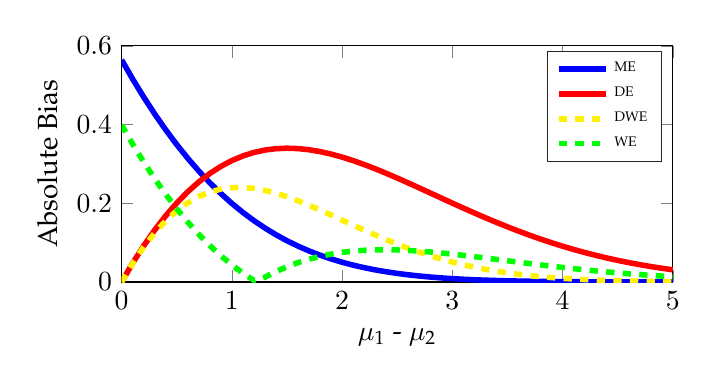
\begin{tikzpicture}

\begin{axis}[%
width=\figurewidth,
height=\figureheight,
at={(0\figurewidth,0\figureheight)},
scale only axis,
xmin=0,
xmax=5,
xlabel={$\mu{}_\text{1}\text{ - }\mu{}_\text{2}$},
ymin=0,
ymax=0.6,
ylabel={Absolute Bias},
axis background/.style={fill=white},
legend style={legend cell align=left,align=left,draw=white!15!black,font=\tiny}
]
\addplot [color=blue,solid,line width=2.0pt]
  table[row sep=crcr]{%
0	0.564189812534416\\
0.1	0.515599648998189\\
0.2	0.469822262092706\\
0.3	0.426836634314534\\
0.4	0.386608077886414\\
0.5	0.349088790836935\\
0.6	0.3142186060885\\
0.7	0.281925699726505\\
0.8	0.252127697137691\\
0.9	0.224732893802751\\
1	0.199641333714366\\
1.1	0.176746276666048\\
1.2	0.155935462256768\\
1.3	0.137092534515943\\
1.4	0.12009836126733\\
1.5	0.10483235524784\\
1.6	0.0911737533842476\\
1.7	0.0790027712005131\\
1.8	0.0682017471865897\\
1.9	0.0586559529264314\\
2	0.0502545818114629\\
2.1	0.0428914300411775\\
2.2	0.0364654067523947\\
2.3	0.0308810856952745\\
2.4	0.0260489755207277\\
2.5	0.0218857979180224\\
2.6	0.0183143862495714\\
2.7	0.0152640368203731\\
2.8	0.0126700974284575\\
2.9	0.0104739965349913\\
3	0.00862294532396869\\
3.1	0.00706963457509751\\
3.2	0.00577201327633769\\
3.3	0.00469282915467956\\
3.4	0.00379926205239756\\
3.5	0.00306296756896417\\
3.6	0.00245881481484238\\
3.7	0.0019653872006603\\
3.8	0.00156423329588311\\
3.9	0.00123958540045224\\
4	0.000978063398190562\\
4.1	0.000768352595620083\\
4.2	0.000600970802494407\\
4.3	0.00046797950293186\\
4.4	0.000362828178883856\\
4.5	0.000280060919750373\\
4.6	0.000215216669613119\\
4.7	0.000164649377818014\\
4.8	0.00012540705872704\\
4.9	9.50847753646436e-05\\
5	7.17655958072765e-05\\
};
\addlegendentry{ME};

\addplot [color=red,solid,line width=2.0pt]
  table[row sep=crcr]{%
0	0\\
0.1	0.0480059274475216\\
0.2	0.0920340656782607\\
0.3	0.132114163306093\\
0.4	0.168295434813582\\
0.5	0.200646023621193\\
0.6	0.229252130867058\\
0.7	0.254217496339241\\
0.8	0.275661470629676\\
0.9	0.293718503496933\\
1	0.308536377537044\\
1.1	0.320274495201664\\
1.2	0.329102547118311\\
1.3	0.335198255174269\\
1.4	0.338747934069719\\
1.5	0.339939864914231\\
1.6	0.338967484000845\\
1.7	0.336025197282184\\
1.8	0.331307261019807\\
1.9	0.325004194340788\\
2	0.317309682181021\\
2.1	0.308403239248337\\
2.2	0.29846458893057\\
2.3	0.287664733914299\\
2.4	0.276166541483759\\
2.5	0.264123810817246\\
2.6	0.251680682614368\\
2.7	0.238971050532002\\
2.8	0.226118152777625\\
2.9	0.213234448173494\\
3	0.200421233664372\\
3.1	0.187769031250052\\
3.2	0.175357445398581\\
3.3	0.163255573975484\\
3.4	0.151522304139958\\
3.5	0.1402067723276\\
3.6	0.129348891940413\\
3.7	0.118979837668689\\
3.8	0.109122699971099\\
3.9	0.099793223057788\\
4	0.0910003461540721\\
4.1	0.0827469544979322\\
4.2	0.0750303822641192\\
4.3	0.0678436090357692\\
4.4	0.0611750787319684\\
4.5	0.0550100434823382\\
4.6	0.0493308169829024\\
4.7	0.0441174389226149\\
4.8	0.0393481006999085\\
4.9	0.0349997084961263\\
5	0.031048269845006\\
};
\addlegendentry{DE};

\addplot [color=yellow,dashed,line width=2.0pt]
  table[row sep=crcr]{%
0	1.56359293183864e-17\\
0.1	0.0471814011105915\\
0.2	0.0887537080937451\\
0.3	0.124800604074924\\
0.4	0.155459482116802\\
0.5	0.180918402090562\\
0.6	0.201411971865877\\
0.7	0.217216280861277\\
0.8	0.228643058333972\\
0.9	0.236033225715193\\
1	0.239750060998038\\
1.1	0.240172148633918\\
1.2	0.23768634553309\\
1.3	0.232680936237943\\
1.4	0.225539164493565\\
1.5	0.216633258850221\\
1.6	0.206319228057767\\
1.7	0.194932150902854\\
1.8	0.182782608707843\\
1.9	0.170153732968665\\
2	0.157299206851127\\
2.1	0.144442088298856\\
2.2	0.131774421805298\\
2.3	0.119457580684881\\
2.4	0.107623227264058\\
2.5	0.0963748395877483\\
2.6	0.0857896714516874\\
2.7	0.07592103522569\\
2.8	0.0668008323663489\\
2.9	0.0584422128310549\\
3	0.0508422797980628\\
3.1	0.0439847634452308\\
3.2	0.0378425866107236\\
3.3	0.0323802833099816\\
3.4	0.0275562196630319\\
3.5	0.0233245743973494\\
3.6	0.0196370966943341\\
3.7	0.016444593859822\\
3.8	0.0136981799041769\\
3.9	0.0113502990936999\\
4	0.0093554699664917\\
4.1	0.00767090320306106\\
4.2	0.00625688051201282\\
4.3	0.00507699519472502\\
4.4	0.00409826299369651\\
4.5	0.00329111272247985\\
4.6	0.00262930647700606\\
4.7	0.00208977773799689\\
4.8	0.00165243454756031\\
4.9	0.00129992125629757\\
5	0.00101738003098112\\
};
\addlegendentry{DWE};

\addplot [color=green,dashed,line width=2.0pt]
  table[row sep=crcr]{%
0	0.398942280052912\\
0.1	0.350437794327982\\
0.2	0.304918114607693\\
0.3	0.262364638281808\\
0.4	0.222746577453385\\
0.5	0.18602127936825\\
0.6	0.152134668423941\\
0.7	0.121021802391743\\
0.8	0.0926075333193295\\
0.9	0.0668072638775738\\
1	0.0435277876827731\\
1.1	0.0226681992095983\\
1.2	0.00412086111881981\\
1.3	0.0122275849273355\\
1.4	0.0264951803285558\\
1.5	0.0388035968970054\\
1.6	0.0492770854877477\\
1.7	0.0580414376955937\\
1.8	0.0652229762042171\\
1.9	0.0709475839700823\\
2	0.0753397837167123\\
2.1	0.0785218780210857\\
2.2	0.0806131573342743\\
2.3	0.0817291837017333\\
2.4	0.0819811537869068\\
2.5	0.0814753489931573\\
2.6	0.0803126683837072\\
2.7	0.0785882503712665\\
2.8	0.0763911812295016\\
2.9	0.0738042872982569\\
3	0.07090400877318\\
3.1	0.0677603495206295\\
3.2	0.0644368991636928\\
3.3	0.0609909201156695\\
3.4	0.0574734942577016\\
3.5	0.0539297303461021\\
3.6	0.0503989905770344\\
3.7	0.0469151924528126\\
3.8	0.0435071125440985\\
3.9	0.0401987260367779\\
4	0.0370095603086348\\
4.1	0.0339550636716517\\
4.2	0.0310469694635575\\
4.3	0.0282936700549741\\
4.4	0.0257005760410928\\
4.5	0.0232704749411324\\
4.6	0.0210038681556807\\
4.7	0.0188992958806059\\
4.8	0.0169536411931422\\
4.9	0.0151624172988336\\
5	0.0135200258586347\\
};
\addlegendentry{WE};

\end{axis}
\end{tikzpicture}%
\\[.4cm]
  % This file was created by matlab2tikz.
%
%The latest updates can be retrieved from
%  http://www.mathworks.com/matlabcentral/fileexchange/22022-matlab2tikz-matlab2tikz
%where you can also make suggestions and rate matlab2tikz.
%
\definecolor{mycolor1}{rgb}{0.00000,0.44700,0.74100}%
\definecolor{mycolor2}{rgb}{0.85000,0.32500,0.09800}%
\definecolor{mycolor3}{rgb}{0.92900,0.69400,0.12500}%
\definecolor{mycolor4}{rgb}{0.49400,0.18400,0.55600}%
%
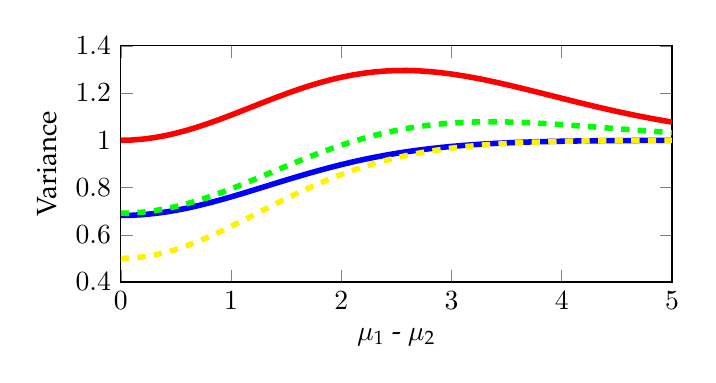
\begin{tikzpicture}

\begin{axis}[%
width=\figurewidth,
height=\figureheight,
at={(0\figurewidth,0\figureheight)},
scale only axis,
xmin=0,
xmax=5,
xlabel={$\mu{}_\text{1}\text{ - }\mu{}_\text{2}$},
ymin=0.4,
ymax=1.4,
ylabel={Variance},
axis background/.style={fill=white}
]
\addplot [color=blue,solid,line width=2.0pt]
  table[row sep=crcr]{%
0	0.681689888923529\\
0.1	0.682597070132036\\
0.2	0.685302679941225\\
0.3	0.689759659487935\\
0.4	0.69589111240446\\
0.5	0.703592709297471\\
0.6	0.712735599233799\\
0.7	0.723169990906402\\
0.8	0.734729524018902\\
0.9	0.747235595458341\\
1	0.760502069940185\\
1.1	0.774339913201566\\
1.2	0.788561624162641\\
1.3	0.802985379149411\\
1.4	0.81743871694557\\
1.5	0.831761686766834\\
1.6	0.845809389611445\\
1.7	0.859453817034573\\
1.8	0.872585364201306\\
1.9	0.885113123098636\\
2	0.896965252865512\\
2.1	0.908088282484715\\
2.2	0.918446258939824\\
2.3	0.928019762293175\\
2.4	0.936803743938235\\
2.5	0.944806485057393\\
2.6	0.952047204263355\\
2.7	0.958554188592952\\
2.8	0.964363332091813\\
2.9	0.96951581700038\\
3	0.974056950834387\\
3.1	0.978034271332406\\
3.2	0.981496391569272\\
3.3	0.984491764270524\\
3.4	0.987067875841473\\
3.5	0.989270280231449\\
3.6	0.991142289141416\\
3.7	0.992724262713452\\
3.8	0.99405354148513\\
3.9	0.995164170701481\\
4	0.996086816594845\\
4.1	0.996849179729348\\
4.2	0.997475595957153\\
4.3	0.997987447839129\\
4.4	0.998403429552356\\
4.5	0.998739668927086\\
4.6	0.999009989724488\\
4.7	0.999226153657174\\
4.8	0.999398085308078\\
4.9	0.999534114911475\\
5	0.999641170862025\\
};

\addplot [color=red,solid,line width=2.0pt]
  table[row sep=crcr]{%
0	1.00000000000711\\
0.1	1.0012479592532\\
0.2	1.00496809890433\\
0.3	1.01108970241045\\
0.4	1.01949706733094\\
0.5	1.03003164772091\\
0.6	1.04249714993544\\
0.7	1.05666260242967\\
0.8	1.0722699956282\\
0.9	1.08903803288274\\
1	1.10667051358046\\
1.1	1.12486374097791\\
1.2	1.14330773320973\\
1.3	1.16170079395562\\
1.4	1.17974970655894\\
1.5	1.1971770141679\\
1.6	1.21372642236551\\
1.7	1.22916710298842\\
1.8	1.24329543279859\\
1.9	1.25594277678604\\
2	1.26696820192132\\
2.1	1.27627025001811\\
2.2	1.28377392287508\\
2.3	1.28944264382208\\
2.4	1.29326977585927\\
2.5	1.29527866487105\\
2.6	1.29551761191069\\
2.7	1.29406184765154\\
2.8	1.29100549960479\\
2.9	1.28646033474802\\
3	1.28055250631444\\
3.1	1.27341841976371\\
3.2	1.26520183058381\\
3.3	1.2560505881951\\
3.4	1.24611352297589\\
3.5	1.23553799054987\\
3.6	1.22446759724444\\
3.7	1.21303953737776\\
3.8	1.20138423466272\\
3.9	1.18962227560482\\
4	1.17786492507654\\
4.1	1.16621227928115\\
4.2	1.15475509825146\\
4.3	1.14356698414854\\
4.4	1.13271841348683\\
4.5	1.12226385257872\\
4.6	1.11224833324996\\
4.7	1.10270687869047\\
4.8	1.09366516306902\\
4.9	1.08514045348215\\
5	1.07714203281135\\
};

\addplot [color=yellow,dashed,line width=2.0pt]
  table[row sep=crcr]{%
0	0.49999999998315\\
0.1	0.501588899927574\\
0.2	0.506323953831822\\
0.3	0.514111323239816\\
0.4	0.524798221630153\\
0.5	0.538178124012069\\
0.6	0.553997773658794\\
0.7	0.571965371346274\\
0.8	0.591760004365354\\
0.9	0.613041432920752\\
1	0.635460055754392\\
1.1	0.658666607447429\\
1.2	0.682321089295853\\
1.3	0.706100829034449\\
1.4	0.729707229123386\\
1.5	0.752871174567479\\
1.6	0.775356920722567\\
1.7	0.796964627413587\\
1.8	0.817531349582231\\
1.9	0.836930858624415\\
2	0.8550723130242\\
2.1	0.871898017701199\\
2.2	0.887380480776571\\
2.3	0.901518968470092\\
2.4	0.914335767894011\\
2.5	0.925872323304705\\
2.6	0.936185374863362\\
2.7	0.945343540714492\\
2.8	0.953423474167446\\
2.9	0.960507270831545\\
3	0.966679576916136\\
3.1	0.972025367813989\\
3.2	0.976628082792492\\
3.3	0.980568143943008\\
3.4	0.98392183349042\\
3.5	0.986760493433565\\
3.6	0.98915001022363\\
3.7	0.991150536963748\\
3.8	0.992816418312007\\
3.9	0.994196273677229\\
4	0.99533320561918\\
4.1	0.99626509696492\\
4.2	0.997024971948696\\
4.3	0.997641395125452\\
4.4	0.998138888796186\\
4.5	0.998538353186855\\
4.6	0.998857476836773\\
4.7	0.999111128377503\\
4.8	0.999311723139144\\
4.9	0.999469560663146\\
5	0.999593130809395\\
};

\addplot [color=green,dashed,line width=2.0pt]
  table[row sep=crcr]{%
0	0.691288022325967\\
0.1	0.692457659357302\\
0.2	0.695948584532084\\
0.3	0.701707255943373\\
0.4	0.709645805833314\\
0.5	0.719644050399147\\
0.6	0.731552214645614\\
0.7	0.745194289472626\\
0.8	0.760371919703622\\
0.9	0.776868705551232\\
1	0.794454793020642\\
1.1	0.81289162655734\\
1.2	0.831936716589637\\
1.3	0.851348323589773\\
1.4	0.870889901510321\\
1.5	0.890334252388781\\
1.6	0.909467216301021\\
1.7	0.928090909505299\\
1.8	0.94602640156318\\
1.9	0.963115815131971\\
2	0.979223830112235\\
2.1	0.994238594929192\\
2.2	1.00807206585465\\
2.3	1.02065980806836\\
2.4	1.03196030884429\\
2.5	1.04195385898313\\
2.6	1.05064106877349\\
2.7	1.05804108805056\\
2.8	1.06418960118502\\
2.9	1.06913666907334\\
3	1.07294448427985\\
3.1	1.07568510351583\\
3.2	1.0774382134563\\
3.3	1.07828897999146\\
3.4	1.07834313123157\\
3.5	1.0776395398492\\
3.6	1.07631963533471\\
3.7	1.07445481866819\\
3.8	1.072130734111\\
3.9	1.06942909385282\\
4	1.06642682111088\\
4.1	1.06319539361385\\
4.2	1.05980037674628\\
4.3	1.05630112905644\\
4.4	1.05275066474352\\
4.5	1.04919565284905\\
4.6	1.04567653494866\\
4.7	1.0422277411383\\
4.8	1.03887798582772\\
4.9	1.03565062518922\\
5	1.03256406000058\\
};

\end{axis}
\end{tikzpicture}%

}
\end{center}
% \end{minipage}
}

%%%%%%%%%%%%%%%%%%%%%%%%%%%%%%%%%%%%%%%%%%%%%%%%%%%%%%%%%%%%%%%%%%%%%%%%%%%%%%
\headerbox{Empirical Results}{name=emp,column=0,row=3,span=6,below=thres}{
% \headerbox{Finite Sample Analysis}{name=settings,column=2,row=0}{
%%%%%%%%%%%%%%%%%%%%%%%%%%%%%%%%%%%%%%%%%%%%%%%%%%%%%%%%%%%%%%%%%%%%%%%%%%%%%%
\begin{minipage}[t]{.49\textwidth}
 \listhead{Multi-Armed Bandits}
 
 \centering \textbf{Internet Ads}\\
   % This file was created by matlab2tikz.
%
%The latest updates can be retrieved from
%  http://www.mathworks.com/matlabcentral/fileexchange/22022-matlab2tikz-matlab2tikz
%where you can also make suggestions and rate matlab2tikz.
%
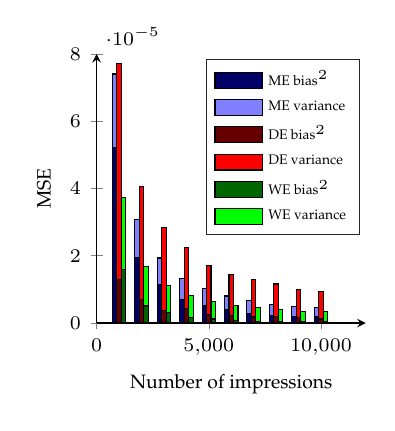
\begin{tikzpicture}

\begin{axis}[%
font=\scriptsize,
width=5cm,
height=5cm,
% at={(0\figurewidth,0\figureheight)},
% scale only axis,
bar width=200,
xmin=0,
xmax=12000,
xlabel={Number of impressions},
ymin=0,
ymax=8e-05,
ylabel={MSE},
ytick align=outside,
xtick align=outside,
axis lines=left,
axis background/.style={fill=white},
scaled x ticks=false,
% axis x line*=bottom,
% axis y line*=left,
legend style={legend cell align=left,font=\tiny,align=left,draw=white!15!black}
]
\addplot[ybar stacked,draw=black,fill=black!60!blue,area legend] plot table[row sep=crcr] {%
800	5.22370101678072e-05\\
1000	0\\
1200	0\\
1800	1.94584364612106e-05\\
2000	0\\
2200	0\\
2800	1.15821211058096e-05\\
3000	0\\
3200	0\\
3800	7.07094653366199e-06\\
4000	0\\
4200	0\\
4800	5.32256275994634e-06\\
5000	0\\
5200	0\\
5800	3.95342806921459e-06\\
6000	0\\
6200	0\\
6800	2.94221705230632e-06\\
7000	0\\
7200	0\\
7800	2.2836432040525e-06\\
8000	0\\
8200	0\\
8800	2.03113186092486e-06\\
9000	0\\
9200	0\\
9800	1.90238811042757e-06\\
10000	0\\
10200	0\\
};
\addlegendentry{ME bias$^2$};

\addplot[ybar stacked,draw=black,fill=white!50!blue,area legend] plot table[row sep=crcr] {%
800	2.17665812408768e-05\\
1000	0\\
1200	0\\
1800	1.14256674925782e-05\\
2000	0\\
2200	0\\
2800	7.73952964113573e-06\\
3000	0\\
3200	0\\
3800	6.23055983153594e-06\\
4000	0\\
4200	0\\
4800	4.96276702262694e-06\\
5000	0\\
5200	0\\
5800	4.10003148472555e-06\\
6000	0\\
6200	0\\
6800	3.81300286670158e-06\\
7000	0\\
7200	0\\
7800	3.34306938892775e-06\\
8000	0\\
8200	0\\
8800	2.9293346514924e-06\\
9000	0\\
9200	0\\
9800	2.76759677773852e-06\\
10000	0\\
10200	0\\
};
\addlegendentry{ME variance};

\addplot[ybar stacked,draw=black,fill=black!60!red,area legend] plot table[row sep=crcr] {%
800	0\\
1000	1.28739169464839e-05\\
1200	0\\
1800	0\\
2000	7.04103512045844e-06\\
2200	0\\
2800	0\\
3000	3.76574985233674e-06\\
3200	0\\
3800	0\\
4000	4.19976651920077e-06\\
4200	0\\
4800	0\\
5000	2.51692513403936e-06\\
5200	0\\
5800	0\\
6000	2.19314499019605e-06\\
6200	0\\
6800	0\\
7000	1.78794168874784e-06\\
7200	0\\
7800	0\\
8000	1.90797852653824e-06\\
8200	0\\
8800	0\\
9000	1.64017337055815e-06\\
9200	0\\
9800	0\\
10000	1.19059916730642e-06\\
12000	0\\
};
\addlegendentry{DE bias$^2$};

\addplot[ybar stacked,draw=black,fill=red,area legend] plot table[row sep=crcr] {%
800	0\\
1000	6.41991851251696e-05\\
1200	0\\
1800	0\\
2000	3.34614145091984e-05\\
2200	0\\
2800	0\\
3000	2.45083818099116e-05\\
3200	0\\
3800	0\\
4000	1.83496173135522e-05\\
4200	0\\
4800	0\\
5000	1.46745781867738e-05\\
5200	0\\
5800	0\\
6000	1.21789631625855e-05\\
6200	0\\
6800	0\\
7000	1.12056626574375e-05\\
7200	0\\
7800	0\\
8000	9.70099613087616e-06\\
8200	0\\
8800	0\\
9000	8.45591203467176e-06\\
9200	0\\
9800	0\\
10000	8.30331990645641e-06\\
12000	0\\
};
\addlegendentry{DE variance};

\addplot[ybar stacked,draw=black,fill=black!60!green,area legend] plot table[row sep=crcr] {%
800	0\\
1000	0\\
1200	1.59944374625979e-05\\
1800	0\\
2000	0\\
2200	5.06156755473435e-06\\
2800	0\\
3000	0\\
3200	3.00415073817953e-06\\
3800	0\\
4000	0\\
4200	1.62348049433556e-06\\
4800	0\\
5000	0\\
5200	1.20660766729076e-06\\
5800	0\\
6000	0\\
6200	8.13695900922474e-07\\
6800	0\\
7000	0\\
7200	5.44253608108319e-07\\
7800	0\\
8000	0\\
8200	3.93589435241593e-07\\
8800	0\\
9000	0\\
9200	3.62064501202791e-07\\
9800	0\\
10000	0\\
10200	3.77081131115167e-07\\
};
\addlegendentry{WE bias$^2$};

\addplot[ybar stacked,draw=black,fill=green,area legend] plot table[row sep=crcr] {%
800	0\\
1000	0\\
1200	2.13429896632014e-05\\
1800	0\\
2000	0\\
2200	1.16277648240915e-05\\
2800	0\\
3000	0\\
3200	8.06037614182458e-06\\
3800	0\\
4000	0\\
4200	6.47003808021854e-06\\
4800	0\\
5000	0\\
5200	5.25519155332697e-06\\
5800	0\\
6000	0\\
6200	4.31657649102447e-06\\
6800	0\\
7000	0\\
7200	4.06236267282256e-06\\
7800	0\\
8000	0\\
8200	3.57429015967058e-06\\
8800	0\\
9000	0\\
9200	3.10939812207049e-06\\
9800	0\\
10000	0\\
10200	3.02132950904338e-06\\
};
\addlegendentry{WE variance};

\end{axis}
\end{tikzpicture}%
\hspace{.1cm}
   % This file was created by matlab2tikz.
%
%The latest updates can be retrieved from
%  http://www.mathworks.com/matlabcentral/fileexchange/22022-matlab2tikz-matlab2tikz
%where you can also make suggestions and rate matlab2tikz.
%
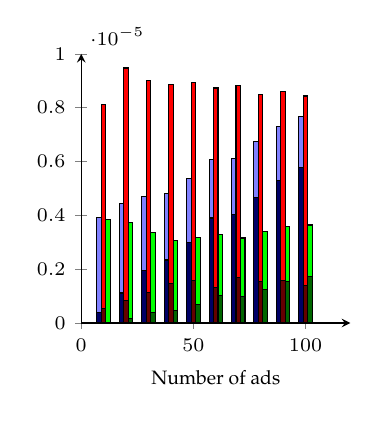
\begin{tikzpicture}

\begin{axis}[%
font=\scriptsize,
width=5cm,
height=5cm,
% at={(0\figurewidth,0\figureheight)},
% scale only axis,
bar width=2,
xmin=0,
xmax=120,
xlabel={Number of ads},
ymin=0,
ymax=1e-05,
axis background/.style={fill=white},
% axis x line*=bottom,
% axis y line*=left,
ytick align=outside,
xtick align=outside,
axis lines=left,
]
\addplot[ybar stacked,draw=black,fill=black!60!blue,area legend] plot table[row sep=crcr] {%
8	3.80693574374186e-07\\
10	0\\
12	0\\
18	1.11443009558663e-06\\
20	0\\
22	0\\
28	1.9499772893414e-06\\
30	0\\
32	0\\
38	2.34265301559432e-06\\
40	0\\
42	0\\
48	2.9901597737099e-06\\
50	0\\
52	0\\
58	3.90428279335706e-06\\
60	0\\
62	0\\
68	4.04393570962261e-06\\
70	0\\
72	0\\
78	4.65296721115062e-06\\
80	0\\
82	0\\
88	5.30297215324858e-06\\
90	0\\
92	0\\
98	5.78366654475033e-06\\
100	0\\
102	0\\
};

\addplot[ybar stacked,draw=black,fill=white!50!blue,area legend] plot table[row sep=crcr] {%
8	3.54373325591694e-06\\
10	0\\
12	0\\
18	3.33524644210525e-06\\
20	0\\
22	0\\
28	2.76622349803199e-06\\
30	0\\
32	0\\
38	2.47288155736491e-06\\
40	0\\
42	0\\
48	2.3783170531094e-06\\
50	0\\
52	0\\
58	2.16352231736602e-06\\
60	0\\
62	0\\
68	2.08122673821169e-06\\
70	0\\
72	0\\
78	2.07700831964199e-06\\
80	0\\
82	0\\
88	1.99621761553372e-06\\
90	0\\
92	0\\
98	1.90498837931974e-06\\
100	0\\
102	0\\
};

\addplot[ybar stacked,draw=black,fill=black!60!red,area legend] plot table[row sep=crcr] {%
8	0\\
10	5.54237506194671e-07\\
12	0\\
18	0\\
20	8.32140988589674e-07\\
22	0\\
28	0\\
30	1.12920899928325e-06\\
32	0\\
38	0\\
40	1.48174355778221e-06\\
42	0\\
48	0\\
50	1.58211447542052e-06\\
52	0\\
58	0\\
60	1.31610422949026e-06\\
62	0\\
68	0\\
70	1.69165852136863e-06\\
72	0\\
78	0\\
80	1.53617740148735e-06\\
82	0\\
88	0\\
90	1.59366013948271e-06\\
92	0\\
98	0\\
100	1.40975931428279e-06\\
102	0\\
};

\addplot[ybar stacked,draw=black,fill=red,area legend] plot table[row sep=crcr] {%
8	0\\
10	7.57051195143716e-06\\
12	0\\
18	0\\
20	8.6447923296027e-06\\
22	0\\
28	0\\
30	7.88565134203441e-06\\
32	0\\
38	0\\
40	7.37726342606092e-06\\
42	0\\
48	0\\
50	7.3510799502365e-06\\
52	0\\
58	0\\
60	7.41778038700625e-06\\
62	0\\
68	0\\
70	7.14584934744175e-06\\
72	0\\
78	0\\
80	6.94560322644048e-06\\
82	0\\
88	0\\
90	6.99886308202045e-06\\
92	0\\
98	0\\
100	7.02410420223558e-06\\
102	0\\
};

\addplot[ybar stacked,draw=black,fill=black!60!green,area legend] plot table[row sep=crcr] {%
8	0\\
10	0\\
12	3.11709599236456e-08\\
18	0\\
20	0\\
22	1.61661015490051e-07\\
28	0\\
30	0\\
32	3.99769513144925e-07\\
38	0\\
40	0\\
42	4.59562851883191e-07\\
48	0\\
50	0\\
52	6.78658211608665e-07\\
58	0\\
60	0\\
62	1.02654671018813e-06\\
68	0\\
70	0\\
72	9.94681753035759e-07\\
78	0\\
80	0\\
82	1.24944286049967e-06\\
88	0\\
90	0\\
92	1.53516836224671e-06\\
98	0\\
100	0\\
102	1.71425662695843e-06\\
};

\addplot[ybar stacked,draw=black,fill=green,area legend] plot table[row sep=crcr] {%
8	0\\
10	0\\
12	3.80188855901277e-06\\
18	0\\
20	0\\
22	3.57246198062572e-06\\
28	0\\
30	0\\
32	2.97113967138879e-06\\
38	0\\
40	0\\
42	2.61933186690901e-06\\
48	0\\
50	0\\
52	2.48322678208886e-06\\
58	0\\
60	0\\
62	2.27657049514232e-06\\
68	0\\
70	0\\
72	2.16461284866537e-06\\
78	0\\
80	0\\
82	2.14635617810677e-06\\
88	0\\
90	0\\
92	2.04242824897428e-06\\
98	0\\
100	0\\
102	1.93021862113537e-06\\
};

\end{axis}
\end{tikzpicture}%
\hspace{.1cm} 
   % This file was created by matlab2tikz.
%
%The latest updates can be retrieved from
%  http://www.mathworks.com/matlabcentral/fileexchange/22022-matlab2tikz-matlab2tikz
%where you can also make suggestions and rate matlab2tikz.
%
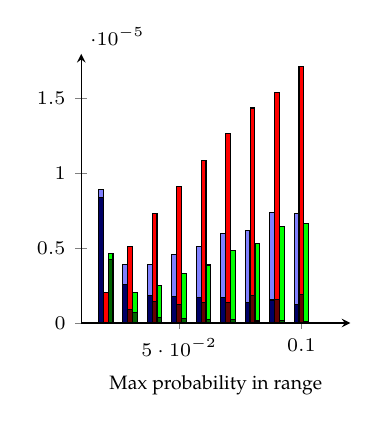
\begin{tikzpicture}

\begin{axis}[%
font=\scriptsize,
width=5cm,
height=5cm,
% at={(0\figurewidth,0\figureheight)},
% scale only axis,
bar width=1.75pt,
xmin=0.01,
xmax=0.12,
xlabel={Max probability in range},
ymin=0,
ymax=1.8e-05,
axis background/.style={fill=white},
% axis x line*=bottom,
% axis y line*=left,
ytick align=outside,
xtick align=outside,
axis lines=left,
scaled x ticks=false
]
\addplot[ybar stacked,draw=black,fill=black!60!blue,area legend] plot table[row sep=crcr] {%
0.018	8.40478081e-06\\
0.02    0\\
0.022    0\\
0.028	2.59951826172461e-06\\
0.03	0\\
0.032	0\\
0.038	1.8211798493316e-06\\
0.04	0\\
0.042	0\\
0.048	1.76420729204589e-06\\
0.05	0\\
0.052	0\\
0.058	1.68881345674181e-06\\
0.06	0\\
0.062	0\\
0.068	1.69931730791119e-06\\
0.07	0\\
0.072	0\\
0.078	1.35866946538677e-06\\
0.080	0\\
0.082	0\\
0.088	1.53835233991489e-06\\
0.09	0\\
0.092	0\\
0.098	1.23504073543409e-06\\
0.1	0\\
0.102	0\\
};

\addplot[ybar stacked,draw=black,fill=white!50!blue,area legend] plot table[row sep=crcr] {%
0.018	5.10934657328664e-07\\
0.02    0\\
0.022   0\\
0.028	1.32727920131091e-06\\
0.03	0\\
0.032	0\\
0.038	2.06684079052236e-06\\
0.04	0\\
0.042	0\\
0.048	2.8180045601331e-06\\
0.05	0\\
0.052	0\\
0.058	3.41172064059962e-06\\
0.06	0\\
0.062	0\\
0.068	4.30706794928735e-06\\
0.07	0\\
0.072	0\\
0.078	4.84212750065487e-06\\
0.08	0\\
0.082	0\\
0.088	5.83999852553997e-06\\
0.09	0\\
0.092	0\\
0.098	6.11293075700731e-06\\
0.100	0\\	
0.102	0\\
};

\addplot[ybar stacked,draw=black,fill=black!60!red,area legend] plot table[row sep=crcr] {%
0.018   0\\
0.02	5.42424100000019e-10\\
0.022   0\\
0.028	0\\
0.03	9.3366709289798e-07\\
0.032	0\\
0.038	0\\
0.04	1.43601643865221e-06\\
0.042	0\\
0.048	0\\
0.05	1.21824275474587e-06\\
0.052	0\\
0.058	0\\
0.06	1.37598321563009e-06\\
0.062	0\\
0.068	0\\
0.07	1.35748833161778e-06\\
0.072	0\\
0.078	0\\
0.08	1.8228291159688e-06\\
0.082	0\\
0.088	0\\
0.09	1.57094055376336e-06\\
0.092	0\\
0.098	0\\
0.1	1.88142683304198e-06\\
0.102	0\\
};

\addplot[ybar stacked,draw=black,fill=red,area legend] plot table[row sep=crcr] {%
0.018   0\\
0.02	2.03442055562225e-06\\
0.022   0\\
0.028	0\\
0.03	4.16751140337695e-06\\
0.032	0\\
0.038	0\\
0.04	5.86817944392382e-06\\
0.042	0\\
0.048	0\\
0.05	7.90820009431466e-06\\
0.052	0\\
0.058	0\\
0.06	9.50276629102284e-06\\
0.062	0\\
0.068	0\\
0.07	1.134634775636e-05\\
0.072	0\\
0.078	0\\
0.08	1.25554645075677e-05\\
0.082	0\\
0.088	0\\
0.09	1.38600160673139e-05\\
0.092	0\\
0.098	0\\
0.1	1.53021848748957e-05\\
0.102	0\\
};

\addplot[ybar stacked,draw=black,fill=black!60!green,area legend] plot table[row sep=crcr] {%
0.018   0\\
0.02    0\\
0.022	4.23230050042347e-06\\
0.028	0\\
0.030	0\\
0.032	6.872739577429e-07\\
0.038	0\\
0.040	0\\
0.042	3.434104977694e-07\\
0.048	0\\
0.050	0\\
0.052	3.21289244759768e-07\\
0.058	0\\
0.060	0\\
0.062	2.59518683896645e-07\\
0.068	0\\
0.070	0\\
0.072	2.60600063723978e-07\\
0.078	0\\
0.080	0\\
0.082	1.38267210772806e-07\\
0.088	0\\
0.090	0\\
0.092	1.86844610529924e-07\\
0.098	0\\
0.01	0\\
0.102	9.34046806333811e-08\\
};

\addplot[ybar stacked,draw=black,fill=green,area legend] plot table[row sep=crcr] {%
0.018   0\\
0.02    0\\
0.022	4.45272799524191e-07\\
0.028	0\\
0.030	0\\
0.032	1.3702607531709e-06\\
0.038	0\\
0.040	0\\
0.042	2.17045652479812e-06\\
0.048	0\\
0.050	0\\
0.052	3.01143246079564e-06\\
0.058	0\\
0.060	0\\
0.062	3.62447165852855e-06\\
0.068	0\\
0.070	0\\
0.072	4.60820180173523e-06\\
0.078	0\\
0.080	0\\
0.082	5.18523820474481e-06\\
0.088	0\\
0.090	0\\
0.092	6.25403179095571e-06\\
0.098	0\\
0.01	0\\
0.102	6.54092714618522e-06\\
};

\end{axis}
\end{tikzpicture}%

   
 \centering \textbf{Sponsored Search Auctions}\\
   % This file was created by matlab2tikz.
%
%The latest updates can be retrieved from
%  http://www.mathworks.com/matlabcentral/fileexchange/22022-matlab2tikz-matlab2tikz
%where you can also make suggestions and rate matlab2tikz.
%
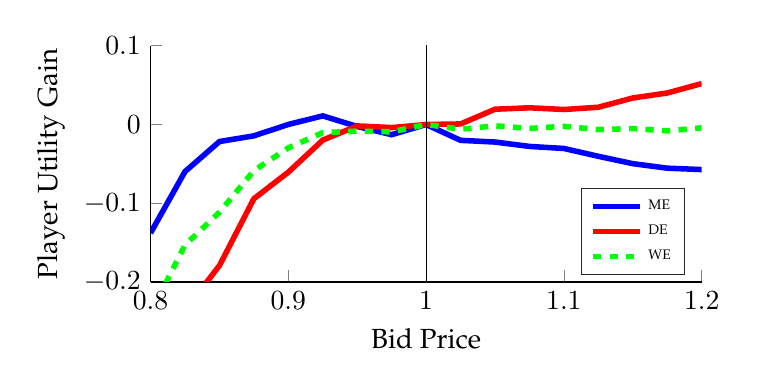
\begin{tikzpicture}

\begin{axis}[%
width=\figurewidth,
height=\figureheight,
at={(0\figurewidth,0\figureheight)},
scale only axis,
xmin=0.8,
xmax=1.2,
xlabel={Bid Price},
ymin=-0.2,
ymax=0.1,
ylabel={Player Utility Gain},
axis background/.style={fill=white},
axis x line*=bottom,
axis y line*=left,
legend style={legend cell align=left,at={(0.97,0.03)},anchor=south east,font=\tiny,align=left,draw=white!15!black}
]
\addplot [color=blue,solid,line width=2.0pt]
  table[row sep=crcr]{%
0.8	-0.137894715666603\\
0.825	-0.0598468461810808\\
0.85	-0.0216533329876517\\
0.875	-0.0143988706450842\\
0.9	7.93661071794016e-05\\
0.925	0.0109612613274912\\
0.95	-0.00253243675744719\\
0.975	-0.0129431164855713\\
1	0\\
1.025	-0.0201081430557002\\
1.05	-0.0222750641676381\\
1.075	-0.027825265848884\\
1.1	-0.0304365443952155\\
1.125	-0.0404001901852189\\
1.15	-0.0497379730112635\\
1.175	-0.0554607211575615\\
1.2	-0.0572394763850563\\
};
\addlegendentry{ME};

\addplot [color=red,solid,line width=2.0pt]
  table[row sep=crcr]{%
0.8	-0.334025140780816\\
0.825	-0.235772413494577\\
0.85	-0.179215364063559\\
0.875	-0.0942457121040257\\
0.9	-0.0605449008581977\\
0.925	-0.0198144078462104\\
0.95	-0.0017729792282466\\
0.975	-0.00390379690928488\\
1	0\\
1.025	0.000709358185508435\\
1.05	0.0194202890798507\\
1.075	0.0212079653200121\\
1.1	0.0190545282083883\\
1.125	0.0219456523943351\\
1.15	0.0336650869436226\\
1.175	0.0400227732745231\\
1.2	0.0519578234196525\\
};
\addlegendentry{DE};

\addplot [color=green,dashed,line width=2.0pt]
  table[row sep=crcr]{%
0.8	-0.239575493584934\\
0.825	-0.153077168367924\\
0.85	-0.111419616118559\\
0.875	-0.0586675334263014\\
0.9	-0.0296467921201244\\
0.925	-0.0103244635296502\\
0.95	-0.00841879231058218\\
0.975	-0.00930787445688375\\
1	0\\
1.025	-0.00602090950513301\\
1.05	-0.00170167090145357\\
1.075	-0.00493446273694942\\
1.1	-0.00228142550333965\\
1.125	-0.00644371658246312\\
1.15	-0.00516778260566453\\
1.175	-0.00808813887417403\\
1.2	-0.00422633762707469\\
};
\addlegendentry{WE};

\addplot [color=black,solid,forget plot]
  table[row sep=crcr]{%
1	-5\\
1	5\\
};
\end{axis}
\end{tikzpicture}%

\end{minipage}\hfill
\begin{minipage}[t]{.525\textwidth}
 \listhead{Markov Decision Processes}

 \centering \textbf{Grid World}\\
   % This file was created by matlab2tikz.
%
%The latest updates can be retrieved from
%  http://www.mathworks.com/matlabcentral/fileexchange/22022-matlab2tikz-matlab2tikz
%where you can also make suggestions and rate matlab2tikz.
%
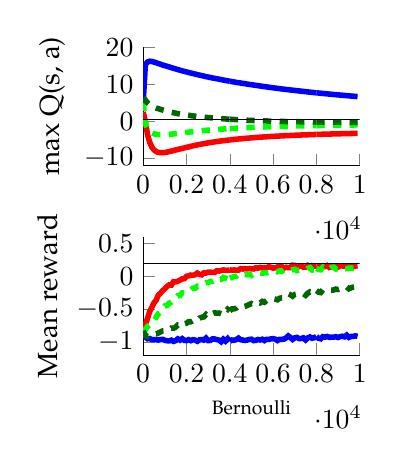
\begin{tikzpicture}
\begin{axis}[%
width=2.75cm,
height=1.5cm,
at={(0\figurewidth,0.591\figureheight)},
scale only axis,
xmin=0,
xmax=10000,
ymin=-1.2,
ymax=0.6,
xlabel style={at={(0.5, -0.3)},font=\scriptsize},
xlabel={Bernoulli},
ylabel style={align=center},
ylabel={Mean reward},
axis background/.style={fill=white},
axis x line*=bottom,
axis y line*=left,
%legend style={at={(0.97,0.2)},anchor=south east,legend cell align=left,align=left,draw=white!15!black,font=\tiny}
]
\addplot [color=blue,solid,line width=2.0pt,forget plot]
  table[row sep=crcr]{%
1	-0.869785\\
101	-0.921757\\
201	-0.950572\\
301	-0.94691\\
401	-0.964509\\
501	-0.963031\\
601	-0.965384\\
701	-0.970065\\
801	-0.962133\\
901	-0.958949\\
1001	-0.973673\\
1101	-0.980448\\
1201	-0.982936\\
1301	-0.971386\\
1401	-0.990054\\
1501	-0.978853\\
1601	-0.951693\\
1701	-0.970812\\
1801	-0.948707\\
1901	-0.974419\\
2001	-0.977892\\
2101	-0.963673999999999\\
2201	-0.979272\\
2301	-0.964846\\
2401	-0.970294\\
2501	-0.98842\\
2601	-0.966674\\
2701	-0.962993\\
2801	-0.9702\\
2901	-0.940511\\
3001	-0.978295\\
3101	-0.975665\\
3201	-0.953603\\
3301	-0.953671\\
3401	-0.96419\\
3501	-0.970474\\
3601	-0.995672\\
3701	-0.957356\\
3801	-0.985595\\
3901	-0.948704\\
4001	-0.986776\\
};
\addplot [color=blue,solid,line width=2.0pt,forget plot]
  table[row sep=crcr]{%
4001	-0.986776\\
4101	-0.969575\\
4201	-0.973455\\
4301	-0.962657\\
4401	-0.940524\\
4501	-0.965519\\
4601	-0.969714\\
4701	-0.976117\\
4801	-0.97008\\
4901	-0.960786\\
5001	-0.957246\\
5101	-0.978773\\
5201	-0.974\\
5301	-0.961356\\
5401	-0.968909\\
5501	-0.957857999999999\\
5601	-0.977723\\
5701	-0.95904\\
5801	-0.960464\\
5901	-0.952241\\
6001	-0.948713\\
6101	-0.956196\\
6201	-0.97742\\
6301	-0.958799\\
6401	-0.958547\\
6501	-0.956034\\
6601	-0.937843\\
6701	-0.907047\\
6801	-0.929701\\
6901	-0.960132\\
7001	-0.936248\\
7101	-0.929217\\
7201	-0.947828\\
7301	-0.946071\\
7401	-0.936026\\
7501	-0.967955\\
7601	-0.937572000000001\\
7701	-0.92251\\
7801	-0.94223\\
7901	-0.934612\\
8001	-0.916357\\
};
\addplot [color=blue,solid,line width=2.0pt]
  table[row sep=crcr]{%
8001	-0.916357\\
8101	-0.943074\\
8201	-0.951069\\
8301	-0.918186\\
8401	-0.925289\\
8501	-0.915596\\
8601	-0.928434\\
8701	-0.925214\\
8801	-0.92544\\
8901	-0.918984\\
9001	-0.930771\\
9101	-0.917445000000001\\
9201	-0.912189\\
9301	-0.921368\\
9401	-0.895732\\
9501	-0.929521\\
9601	-0.915296\\
9701	-0.913288\\
9801	-0.906296\\
9901	-0.913844\\
};
%\addlegendentry{QL};
\addplot [color=red,solid,line width=2.0pt,forget plot]
  table[row sep=crcr]{%
1	-0.807935\\
101	-0.731633\\
201	-0.640325\\
301	-0.534694\\
401	-0.470654\\
501	-0.400845\\
601	-0.362044\\
701	-0.284939\\
801	-0.256151\\
901	-0.2167\\
1001	-0.187573\\
1101	-0.154114\\
1201	-0.128616\\
1301	-0.131966\\
1401	-0.080981\\
1501	-0.08323\\
1601	-0.073167\\
1701	-0.057204\\
1801	-0.03744\\
1901	-0.035126\\
2001	0.001447\\
2101	0.007876\\
2201	0.020981\\
2301	0.017896\\
2401	0.02605\\
2501	0.050166\\
2601	0.031095\\
2701	0.023924\\
2801	0.053181\\
2901	0.051354\\
3001	0.064127\\
3101	0.065839\\
3201	0.06094\\
3301	0.060194\\
3401	0.086493\\
3501	0.081686\\
3601	0.088428\\
3701	0.099784\\
3801	0.092748\\
3901	0.09339\\
4001	0.099318\\
};
\addplot [color=red,solid,line width=2.0pt,forget plot]
  table[row sep=crcr]{%
4001	0.099318\\
4101	0.095338\\
4201	0.098284\\
4301	0.09437\\
4401	0.096829\\
4501	0.118169\\
4601	0.11161\\
4701	0.117883\\
4801	0.113831\\
4901	0.120222\\
5001	0.114544\\
5101	0.113384\\
5201	0.131359\\
5301	0.12636\\
5401	0.13706\\
5501	0.128365\\
5601	0.132287\\
5701	0.133673\\
5801	0.146524\\
5901	0.139182\\
6001	0.127241\\
6101	0.129954\\
6201	0.143877\\
6301	0.155793\\
6401	0.149781\\
6501	0.12685\\
6601	0.139665\\
6701	0.133907\\
6801	0.135451\\
6901	0.171438\\
7001	0.167533\\
7101	0.133484\\
7201	0.15433\\
7301	0.16014\\
7401	0.13929\\
7501	0.140511\\
7601	0.166008\\
7701	0.144047\\
7801	0.163405\\
7901	0.153165\\
8001	0.159325\\
};
\addplot [color=red,solid,line width=2.0pt]
  table[row sep=crcr]{%
8001	0.159325\\
8101	0.159121\\
8201	0.143995\\
8301	0.150508\\
8401	0.148708\\
8501	0.165621\\
8601	0.137092\\
8701	0.148842\\
8801	0.158943\\
8901	0.158151\\
9001	0.142272\\
9101	0.161048\\
9201	0.158861\\
9301	0.155045\\
9401	0.149346\\
9501	0.150425\\
9601	0.156752\\
9701	0.146362\\
9801	0.15824\\
9901	0.162017\\
};
%\addlegendentry{DQL};
\addplot [color=green,dashed,line width=2.0pt,forget plot]
  table[row sep=crcr]{%
1	-0.811139\\
101	-0.814146\\
201	-0.761311\\
301	-0.736411\\
401	-0.688075\\
501	-0.673952\\
601	-0.619232\\
701	-0.568396\\
801	-0.540216\\
901	-0.506577\\
1001	-0.450202\\
1101	-0.442622\\
1201	-0.407417\\
1301	-0.391702\\
1401	-0.357409\\
1501	-0.338546\\
1601	-0.295783\\
1701	-0.290741\\
1801	-0.25068\\
1901	-0.247708\\
2001	-0.232347\\
2101	-0.206057\\
2201	-0.210812\\
2301	-0.178719\\
2401	-0.178731\\
2501	-0.149092\\
2601	-0.153448\\
2701	-0.123163\\
2801	-0.111361\\
2901	-0.095223\\
3001	-0.095859\\
3101	-0.077966\\
3201	-0.076347\\
3301	-0.059872\\
3401	-0.080973\\
3501	-0.044383\\
3601	-0.046106\\
3701	-0.015342\\
3801	-0.027227\\
3901	-0.040339\\
4001	-0.02585\\
};
\addplot [color=green,dashed,line width=2.0pt,forget plot]
  table[row sep=crcr]{%
4001	-0.02585\\
4101	-0.014219\\
4201	-0.000768000000000003\\
4301	0.001897\\
4401	0.024986\\
4501	0.005362\\
4601	0.013181\\
4701	0.030459\\
4801	0.024737\\
4901	0.033338\\
5001	0.015419\\
5101	0.040286\\
5201	0.033693\\
5301	0.050325\\
5401	0.052924\\
5501	0.046664\\
5601	0.057776\\
5701	0.055719\\
5801	0.061397\\
5901	0.062057\\
6001	0.064551\\
6101	0.082375\\
6201	0.070162\\
6301	0.0861599999999999\\
6401	0.077844\\
6501	0.101863\\
6601	0.092101\\
6701	0.075832\\
6801	0.08372\\
6901	0.100593\\
7001	0.10807\\
7101	0.08764\\
7201	0.0939329999999999\\
7301	0.094918\\
7401	0.087009\\
7501	0.097319\\
7601	0.119655\\
7701	0.134011\\
7801	0.096776\\
7901	0.100561\\
8001	0.121977\\
};
\addplot [color=green,dashed,line width=2.0pt]
  table[row sep=crcr]{%
8001	0.121977\\
8101	0.105337\\
8201	0.10069\\
8301	0.141694\\
8401	0.117275\\
8501	0.128663\\
8601	0.114854\\
8701	0.137614\\
8801	0.140631\\
8901	0.112649\\
9001	0.116239\\
9101	0.113519\\
9201	0.137413\\
9301	0.11854\\
9401	0.117833\\
9501	0.126174\\
9601	0.127922\\
9701	0.121198\\
9801	0.132613\\
9901	0.137484\\
};
%\addlegendentry{WQL};

\addplot [color=black!60!green,dashed,line width=2.0pt,forget plot]
  table[row sep=crcr]{%
1	-0.830087999999999\\
101	-0.897925\\
201	-0.915108\\
301	-0.890162\\
401	-0.89575\\
501	-0.876989\\
601	-0.876323\\
701	-0.86316\\
801	-0.845345\\
901	-0.83046\\
1001	-0.828686\\
1101	-0.823416\\
1201	-0.814653\\
1301	-0.787564\\
1401	-0.790708\\
1501	-0.772282\\
1601	-0.74134\\
1701	-0.746766\\
1801	-0.706518\\
1901	-0.722354000000001\\
2001	-0.713192\\
2101	-0.689465\\
2201	-0.692147\\
2301	-0.672509\\
2401	-0.663053\\
2501	-0.674731\\
2601	-0.636124\\
2701	-0.622799\\
2801	-0.617633\\
2901	-0.58061\\
3001	-0.606169\\
3101	-0.594179\\
3201	-0.566802\\
3301	-0.55361\\
3401	-0.561126\\
3501	-0.558129\\
3601	-0.570288\\
3701	-0.527166\\
3801	-0.540404\\
3901	-0.50028\\
4001	-0.524597\\
};
\addplot [color=black!60!green,dashed,line width=2.0pt,forget plot]
  table[row sep=crcr]{%
4001	-0.524597\\
4101	-0.496173\\
4201	-0.495013\\
4301	-0.48185\\
4401	-0.451026\\
4501	-0.460769\\
4601	-0.464363\\
4701	-0.455074\\
4801	-0.444077\\
4901	-0.428589\\
5001	-0.41288\\
5101	-0.428716\\
5201	-0.421694\\
5301	-0.394971\\
5401	-0.404764\\
5501	-0.380714\\
5601	-0.394457\\
5701	-0.368576\\
5801	-0.362012\\
5901	-0.354186\\
6001	-0.337419\\
6101	-0.346229\\
6201	-0.356431\\
6301	-0.332817\\
6401	-0.327068\\
6501	-0.327411\\
6601	-0.299102\\
6701	-0.264791\\
6801	-0.280106\\
6901	-0.302018\\
7001	-0.275077\\
7101	-0.269171\\
7201	-0.281758\\
7301	-0.277673\\
7401	-0.263838\\
7501	-0.287831\\
7601	-0.25639\\
7701	-0.23503\\
7801	-0.247271\\
7901	-0.240988\\
8001	-0.216298\\
};
\addplot [color=black!60!green,dashed,line width=2.0pt]
  table[row sep=crcr]{%
8001	-0.216298\\
8101	-0.239245\\
8201	-0.246528\\
8301	-0.204331\\
8401	-0.211193\\
8501	-0.210786\\
8601	-0.209248\\
8701	-0.210801\\
8801	-0.20598\\
8901	-0.192817\\
9001	-0.199361\\
9101	-0.188242\\
9201	-0.17914\\
9301	-0.183003\\
9401	-0.160013\\
9501	-0.188757\\
9601	-0.173234\\
9701	-0.163613\\
9801	-0.159591\\
9901	-0.164335\\
};
%\addlegendentry{WQL with W-policy};

\addplot [color=black,solid,forget plot]
  table[row sep=crcr]{%
0	0.2\\
10000	0.2\\
};

\end{axis}
\begin{axis}[%
width=2.75cm,
height=1.5cm,
at={(0\figurewidth,0\figureheight)},
scale only axis,
%xlabel={Number of Steps},
xmin=0,
xmax=10000,
ymin=-12,
ymax=20,
ylabel={max Q(s, a)},
axis background/.style={fill=white},
axis x line*=bottom,
axis y line*=left,
%legend style={legend cell align=left,align=left,draw=white!15!black}
]
\addplot [color=blue,solid,line width=2.0pt,forget plot]
  table[row sep=crcr]{%
1	5.042\\
101	15.319899226743\\
201	16.0466835225602\\
301	16.2494829057667\\
401	16.176420616514\\
501	16.0118915075627\\
601	15.8400272609695\\
701	15.6120464324933\\
801	15.4373093083967\\
901	15.2226867952347\\
1001	15.0425883931108\\
1101	14.8695384131687\\
1201	14.6967457760906\\
1301	14.501909821017\\
1401	14.3321993138159\\
1501	14.1587319824658\\
1601	13.9876696783888\\
1701	13.8117949243584\\
1801	13.6421008587999\\
1901	13.4976590626358\\
2001	13.3391157051725\\
2101	13.2008793739587\\
2201	13.0559708509495\\
2301	12.9009387082866\\
2401	12.7677049017769\\
2501	12.6327637231171\\
2601	12.4860419311218\\
2701	12.3549319963004\\
2801	12.2225142325902\\
2901	12.0798527553591\\
3001	11.9610990380752\\
3101	11.8352562251916\\
3201	11.7143091942766\\
3301	11.599838223871\\
3401	11.5065809698864\\
3501	11.3928077644121\\
3601	11.274282776188\\
3701	11.142470608291\\
3801	11.0468243372339\\
3901	10.9362944234727\\
4001	10.8349490849332\\
};
\addplot [color=blue,solid,line width=2.0pt,forget plot]
  table[row sep=crcr]{%
4001	10.8349490849332\\
4101	10.7220473212542\\
4201	10.6246178296714\\
4301	10.5108720065011\\
4401	10.4289105412492\\
4501	10.339496801428\\
4601	10.2520827624305\\
4701	10.1630572276974\\
4801	10.051182885258\\
4901	9.96433431530049\\
5001	9.88418061014095\\
5101	9.80065750566116\\
5201	9.71389912209656\\
5301	9.62686386736556\\
5401	9.53866578616725\\
5501	9.45590567247928\\
5601	9.37389440104621\\
5701	9.29020477973478\\
5801	9.20304171725133\\
5901	9.12278279494542\\
6001	9.04787566545145\\
6101	8.96574583506793\\
6201	8.89764755463194\\
6301	8.81991867603436\\
6401	8.74175406944385\\
6501	8.67365755123537\\
6601	8.60122045805111\\
6701	8.53069049578859\\
6801	8.46027788859009\\
6901	8.39825215483604\\
7001	8.33044183856243\\
7101	8.25771323416857\\
7201	8.2010772312599\\
7301	8.12850689189653\\
7401	8.06490765366854\\
7501	8.00006086378918\\
7601	7.92989975972565\\
7701	7.86895532734051\\
7801	7.80862589098597\\
7901	7.74557693875408\\
8001	7.68373370069017\\
};
\addplot [color=blue,solid,line width=2.0pt]
  table[row sep=crcr]{%
8001	7.68373370069017\\
8101	7.63170291246204\\
8201	7.56881034914234\\
8301	7.51261470563813\\
8401	7.45919596588956\\
8501	7.39831182406262\\
8601	7.34176005674493\\
8701	7.28284697248715\\
8801	7.2283892051005\\
8901	7.1765838694377\\
9001	7.12453573537874\\
9101	7.07937902663157\\
9201	7.02633662941909\\
9301	6.97548079569124\\
9401	6.92177618627564\\
9501	6.86893785176936\\
9601	6.81886423062493\\
9701	6.76946238423119\\
9801	6.71462285255652\\
9901	6.6674734983616\\
};
%\addlegendentry{Q-Learning};
\addplot [color=red,solid,line width=2.0pt,forget plot]
  table[row sep=crcr]{%
1	2.501\\
101	-0.0849461144702478\\
201	-3.61522861986604\\
301	-5.69906138997146\\
401	-7.00159704615445\\
501	-7.76935234105676\\
601	-8.22228297884329\\
701	-8.46310219288963\\
801	-8.53782983862944\\
901	-8.53839127494341\\
1001	-8.4826937481687\\
1101	-8.37972090315019\\
1201	-8.23560201152564\\
1301	-8.09905966246885\\
1401	-7.94733202283554\\
1501	-7.80301632490966\\
1601	-7.6564503475539\\
1701	-7.51977616338245\\
1801	-7.38708889291362\\
1901	-7.23726111594259\\
2001	-7.09706677143842\\
2101	-6.9563663436873\\
2201	-6.80775870473694\\
2301	-6.67484901973841\\
2401	-6.54682271010947\\
2501	-6.42744979681516\\
2601	-6.30585310083246\\
2701	-6.19615439596569\\
2801	-6.08620652774395\\
2901	-5.97825509268349\\
3001	-5.872555440358\\
3101	-5.77868080285588\\
3201	-5.68863718710495\\
3301	-5.60723866364571\\
3401	-5.51897022665665\\
3501	-5.43255163957478\\
3601	-5.35399497004103\\
3701	-5.28665200075482\\
3801	-5.21761374361836\\
3901	-5.13871017780174\\
4001	-5.07180178579774\\
};
\addplot [color=red,solid,line width=2.0pt,forget plot]
  table[row sep=crcr]{%
4001	-5.07180178579774\\
4101	-5.00387757097217\\
4201	-4.94237110804853\\
4301	-4.88201678147908\\
4401	-4.82297203128923\\
4501	-4.77322916835818\\
4601	-4.71756724834031\\
4701	-4.66161156574933\\
4801	-4.60903959233958\\
4901	-4.56184231209989\\
5001	-4.51109438347685\\
5101	-4.46616961128916\\
5201	-4.41709093911085\\
5301	-4.3715633338612\\
5401	-4.33220085930549\\
5501	-4.29323422974526\\
5601	-4.25441198339821\\
5701	-4.22079751965677\\
5801	-4.18104717521716\\
5901	-4.1447812136826\\
6001	-4.11186458626123\\
6101	-4.080776206142\\
6201	-4.04976193000075\\
6301	-4.01512231829892\\
6401	-3.98302788904876\\
6501	-3.94994333644363\\
6601	-3.92047555245799\\
6701	-3.89263633369541\\
6801	-3.86918298465001\\
6901	-3.846081748016\\
7001	-3.81679844554559\\
7101	-3.78633218169743\\
7201	-3.76472857923167\\
7301	-3.74093239796682\\
7401	-3.71833543277135\\
7501	-3.69618564502953\\
7601	-3.67440190902728\\
7701	-3.65325626445828\\
7801	-3.63316235028871\\
7901	-3.60920392690866\\
8001	-3.58993650388271\\
};
\addplot [color=red,solid,line width=2.0pt]
  table[row sep=crcr]{%
8001	-3.58993650388271\\
8101	-3.56841400621118\\
8201	-3.55075693353316\\
8301	-3.53456592728317\\
8401	-3.51957283417105\\
8501	-3.50191091645451\\
8601	-3.48159157893185\\
8701	-3.46627356439617\\
8801	-3.45040551624311\\
8901	-3.43422120097807\\
9001	-3.41607944451932\\
9101	-3.40309200036275\\
9201	-3.38709380623317\\
9301	-3.37520410575702\\
9401	-3.36332452227671\\
9501	-3.35032367282012\\
9601	-3.33719424365242\\
9701	-3.32429332975784\\
9801	-3.31146603659421\\
9901	-3.29899043405085\\
};
%\addlegendentry{Double Q-Learning};
\addplot [color=green,dashed,line width=2.0pt,forget plot]
  table[row sep=crcr]{%
1	5.019\\
101	-0.561435513976316\\
201	-2.10748613399273\\
301	-2.78850447774576\\
401	-3.15700487049358\\
501	-3.41174133190754\\
601	-3.55697462169387\\
701	-3.64239480258186\\
801	-3.66795806361057\\
901	-3.67724664921577\\
1001	-3.64644698653742\\
1101	-3.61277239919404\\
1201	-3.56879033160159\\
1301	-3.49381167985975\\
1401	-3.45084973825673\\
1501	-3.3849234246058\\
1601	-3.31680884158586\\
1701	-3.23177894881246\\
1801	-3.17111173269135\\
1901	-3.10378626204035\\
2001	-3.03193622140028\\
2101	-2.97144855489982\\
2201	-2.8932340482529\\
2301	-2.8462607211846\\
2401	-2.78700576631412\\
2501	-2.71513363688848\\
2601	-2.64632690525657\\
2701	-2.5858051297294\\
2801	-2.5318372678312\\
2901	-2.47459453842289\\
3001	-2.42609290108204\\
3101	-2.37708271674699\\
3201	-2.33246743219082\\
3301	-2.28554812856573\\
3401	-2.24663166255938\\
3501	-2.21173614704855\\
3601	-2.15535744188794\\
3701	-2.1175579487116\\
3801	-2.07418715019048\\
3901	-2.03088161320522\\
4001	-2.0071391301036\\
};
\addplot [color=green,dashed,line width=2.0pt,forget plot]
  table[row sep=crcr]{%
4001	-2.0071391301036\\
4101	-1.96704703812349\\
4201	-1.9394182915683\\
4301	-1.90579621899051\\
4401	-1.87230738470192\\
4501	-1.83959706586264\\
4601	-1.80904558758474\\
4701	-1.7833779582152\\
4801	-1.75413944462948\\
4901	-1.728073090836\\
5001	-1.7096450189774\\
5101	-1.68508947281969\\
5201	-1.65664616137222\\
5301	-1.62735682515695\\
5401	-1.6018417810666\\
5501	-1.58069805133749\\
5601	-1.56010598341352\\
5701	-1.53959571924263\\
5801	-1.51592903607401\\
5901	-1.49357353944957\\
6001	-1.47202400917923\\
6101	-1.45197229047673\\
6201	-1.43349517897839\\
6301	-1.418755285836\\
6401	-1.39742157282384\\
6501	-1.38095685369288\\
6601	-1.36542725529353\\
6701	-1.34331003529169\\
6801	-1.33120162284379\\
6901	-1.31946723524201\\
7001	-1.30438788861875\\
7101	-1.29050499203282\\
7201	-1.27650701422963\\
7301	-1.26054008061624\\
7401	-1.24306754185121\\
7501	-1.23501307730128\\
7601	-1.22321168459468\\
7701	-1.21437185081218\\
7801	-1.20350948862594\\
7901	-1.19518625004285\\
8001	-1.18459430248304\\
};
\addplot [color=green,dashed,line width=2.0pt]
  table[row sep=crcr]{%
8001	-1.18459430248304\\
8101	-1.1733591045408\\
8201	-1.16139088277911\\
8301	-1.15596448096268\\
8401	-1.14471802345029\\
8501	-1.13560578755813\\
8601	-1.12716944235878\\
8701	-1.11761240314586\\
8801	-1.11044349597731\\
8901	-1.09860608368536\\
9001	-1.08918726865224\\
9101	-1.07906045677369\\
9201	-1.07303305629896\\
9301	-1.06355184611126\\
9401	-1.05518608357189\\
9501	-1.04543337713814\\
9601	-1.03791345089536\\
9701	-1.0312212864366\\
9801	-1.02185498561993\\
9901	-1.01402324986625\\
};

%\addlegendentry{Weighted Q-Learning};
\addplot [color=black!60!green,dashed,line width=2.0pt,forget plot]
  table[row sep=crcr]{%
1	5.042\\
101	5.72736214256866\\
201	4.99068567356508\\
301	4.46778367185515\\
401	4.08935817539066\\
501	3.80224574048378\\
601	3.56191794724855\\
701	3.38433754190323\\
801	3.19575497103867\\
901	3.02768764672756\\
1001	2.86452457696108\\
1101	2.70336351712489\\
1201	2.56241370430275\\
1301	2.42390938789168\\
1401	2.29840075624031\\
1501	2.16941270071875\\
1601	2.04067718297179\\
1701	1.93262813933324\\
1801	1.85667967612719\\
1901	1.7765986210532\\
2001	1.68765230000701\\
2101	1.60445024256116\\
2201	1.51401746174015\\
2301	1.42291990343896\\
2401	1.35266649262799\\
2501	1.27833273987307\\
2601	1.20132451566666\\
2701	1.14497730423841\\
2801	1.0949664482371\\
2901	1.03136809530666\\
3001	0.981640871736366\\
3101	0.934253668490374\\
3201	0.874403100633434\\
3301	0.836392131356486\\
3401	0.791249858079448\\
3501	0.743716341639799\\
3601	0.702594500569252\\
3701	0.658175917127342\\
3801	0.608309044892269\\
3901	0.562871588005203\\
4001	0.530962266430353\\
};
\addplot [color=black!60!green,dashed,line width=2.0pt,forget plot]
  table[row sep=crcr]{%
4001	0.530962266430353\\
4101	0.493624914233332\\
4201	0.459348282445108\\
4301	0.420038099086359\\
4401	0.389140139133673\\
4501	0.356613741846215\\
4601	0.326919821360786\\
4701	0.295178946533069\\
4801	0.258276101225878\\
4901	0.231244219943345\\
5001	0.212017355417852\\
5101	0.184329775196301\\
5201	0.163401335173811\\
5301	0.143853351214861\\
5401	0.117267527974985\\
5501	0.0925523633686421\\
5601	0.0666816472140594\\
5701	0.0555793398466231\\
5801	0.0376473933773014\\
5901	0.0244624385225204\\
6001	0.00522331691579186\\
6101	-0.0127050975797546\\
6201	-0.0312975527044521\\
6301	-0.0515128545815796\\
6401	-0.0683589789490213\\
6501	-0.076824166423207\\
6601	-0.0956919206101078\\
6701	-0.101074834334617\\
6801	-0.105745750639971\\
6901	-0.115847629698052\\
7001	-0.125209715161398\\
7101	-0.13678778766092\\
7201	-0.1456744680606\\
7301	-0.156548138623361\\
7401	-0.168549475529892\\
7501	-0.17682274612283\\
7601	-0.188072307481443\\
7701	-0.196365652379585\\
7801	-0.203034446783482\\
7901	-0.209838398816235\\
8001	-0.217313605696108\\
};
\addplot [color=black!60!green,dashed,line width=2.0pt]
  table[row sep=crcr]{%
8001	-0.217313605696108\\
8101	-0.221098513710607\\
8201	-0.227419152276832\\
8301	-0.228781778396871\\
8401	-0.236607135488062\\
8501	-0.244698427344637\\
8601	-0.251750356024199\\
8701	-0.25747806779048\\
8801	-0.264043446628184\\
8901	-0.270083034576012\\
9001	-0.275720974643646\\
9101	-0.28847651084412\\
9201	-0.289801178957549\\
9301	-0.291705376799069\\
9401	-0.296192777584145\\
9501	-0.298223117933324\\
9601	-0.304460128001615\\
9701	-0.309160001795222\\
9801	-0.309821668751495\\
9901	-0.31856868034202\\
};
%\addlegendentry{W Q-Learning with W-policy};

\addplot [color=black,solid,forget plot]
  table[row sep=crcr]{%
0	0.36\\
10000	0.36\\
};

\end{axis}
\end{tikzpicture}%

   % This file was created by matlab2tikz.
%
%The latest updates can be retrieved from
%  http://www.mathworks.com/matlabcentral/fileexchange/22022-matlab2tikz-matlab2tikz
%where you can also make suggestions and rate matlab2tikz.
%
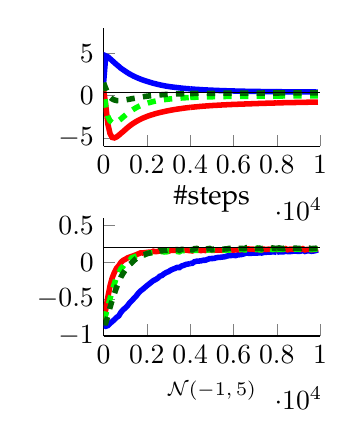
\begin{tikzpicture}
\begin{axis}[%
width=2.75cm,
height=1.5cm,
at={(0\figurewidth,0.591\figureheight)},
scale only axis,
xmin=0,
xmax=10000,
xlabel style={at={(0.5, -0.3)},font=\scriptsize},
xlabel={$\mathcal{N}(-1, 5)$},
ymin=-1,
ymax=0.6,
axis background/.style={fill=white},
axis x line*=bottom,
axis y line*=left,
%legend style={at={(0.97,0.03)},anchor=south east,legend cell align=left,align=left,draw=white!15!black}
]
\addplot [color=blue,solid,line width=2.0pt,forget plot]
  table[row sep=crcr]{%
1	-0.855257798255006\\
101	-0.868656135999948\\
201	-0.858561732400003\\
301	-0.829019806960498\\
401	-0.803835972209468\\
501	-0.778240038785783\\
601	-0.748712487822429\\
701	-0.727671455609818\\
801	-0.679266262762017\\
901	-0.645409730333842\\
1001	-0.620729639625794\\
1101	-0.591402413075512\\
1201	-0.552378606740005\\
1301	-0.523755844442702\\
1401	-0.490575439030471\\
1501	-0.46020885584098\\
1601	-0.422137111753343\\
1701	-0.39083053135822\\
1801	-0.369089602841586\\
1901	-0.344240786314448\\
2001	-0.318571528253216\\
2101	-0.295907239606595\\
2201	-0.272271622713994\\
2301	-0.249499005241066\\
2401	-0.235480607136323\\
2501	-0.216636447688953\\
2601	-0.190240175330748\\
2701	-0.178958089062055\\
2801	-0.155830177468392\\
2901	-0.139031371055162\\
3001	-0.127113119226983\\
3101	-0.108420439277577\\
3201	-0.0950989358046942\\
3301	-0.0844012815407418\\
3401	-0.0703387647588829\\
3501	-0.0736550833274254\\
3601	-0.0518050309884997\\
3701	-0.0434438714492374\\
3801	-0.0304065009594142\\
3901	-0.0251425774152808\\
4001	-0.0181824817697089\\
};
\addplot [color=blue,solid,line width=2.0pt,forget plot]
  table[row sep=crcr]{%
4001	-0.0181824817697089\\
4101	-0.014240901000277\\
4201	0.00680632861478059\\
4301	0.0129729068092121\\
4401	0.0150398107160291\\
4501	0.018207040626123\\
4601	0.0259899005567685\\
4701	0.0263900088169949\\
4801	0.0375368770901541\\
4901	0.0489159937398698\\
5001	0.0497635953466609\\
5101	0.0504251797344635\\
5201	0.0600953644338482\\
5301	0.0644965730131224\\
5401	0.0667131435486074\\
5501	0.0698030466609577\\
5601	0.0734296040284437\\
5701	0.0833467437018226\\
5801	0.089256831583371\\
5901	0.0906161184824017\\
6001	0.0926292317723521\\
6101	0.0891844867793839\\
6201	0.0987665139870463\\
6301	0.101141182006002\\
6401	0.105414838182257\\
6501	0.114342851591457\\
6601	0.125314814534639\\
6701	0.120293472139562\\
6801	0.120177918063778\\
6901	0.122817029066532\\
7001	0.123067614959693\\
7101	0.12348851408078\\
7201	0.128404758374055\\
7301	0.123894438082438\\
7401	0.132160432211827\\
7501	0.134441294525234\\
7601	0.13545186111112\\
7701	0.135292084532101\\
7801	0.142619788900605\\
7901	0.138777743566843\\
8001	0.132195538904142\\
};
\addplot [color=blue,solid,line width=2.0pt]
  table[row sep=crcr]{%
8001	0.132195538904142\\
8101	0.14147292358699\\
8201	0.138512725891396\\
8301	0.138987301687328\\
8401	0.149707957971578\\
8501	0.143586026120537\\
8601	0.142472381597223\\
8701	0.147499100145233\\
8801	0.149749997695686\\
8901	0.148664663840338\\
9001	0.146347660495827\\
9101	0.148804539565755\\
9201	0.159485906858081\\
9301	0.145591369162092\\
9401	0.153495001438605\\
9501	0.153485593344225\\
9601	0.147457537438557\\
9701	0.151289522913154\\
9801	0.157394035579814\\
9901	0.165535667691785\\
};
%\addlegendentry{Q-Learning};
\addplot [color=red,solid,line width=2.0pt,forget plot]
  table[row sep=crcr]{%
1	-0.779643810243355\\
101	-0.637604611151465\\
201	-0.467384562563498\\
301	-0.31808567770842\\
401	-0.210879256451165\\
501	-0.138061161929467\\
601	-0.0819995987793671\\
701	-0.0470135124045073\\
801	-0.00345379838445892\\
901	0.0246090294039716\\
1001	0.0386238961870837\\
1101	0.0574574766048244\\
1201	0.0690734001537133\\
1301	0.0784340737530138\\
1401	0.0886737804982378\\
1501	0.100301806612439\\
1601	0.112782010965231\\
1701	0.125231584902996\\
1801	0.124472015928138\\
1901	0.129446119936963\\
2001	0.132111793242008\\
2101	0.13609181612797\\
2201	0.135008254859294\\
2301	0.148423038417101\\
2401	0.142136759616271\\
2501	0.145808062139282\\
2601	0.15336259431507\\
2701	0.148176868863585\\
2801	0.152691344149943\\
2901	0.150590483075908\\
3001	0.147748208156069\\
3101	0.160770836721944\\
3201	0.158869848146359\\
3301	0.158891432954166\\
3401	0.160819696342081\\
3501	0.150443085079902\\
3601	0.164664149149879\\
3701	0.161563165208242\\
3801	0.165193941438132\\
3901	0.158743955635513\\
4001	0.157119898327302\\
};
\addplot [color=red,solid,line width=2.0pt,forget plot]
  table[row sep=crcr]{%
4001	0.157119898327302\\
4101	0.152671393575049\\
4201	0.169658737596327\\
4301	0.171497564424005\\
4401	0.161929919742241\\
4501	0.157104088957867\\
4601	0.164062798865747\\
4701	0.157757156204209\\
4801	0.167117382451234\\
4901	0.167109823566255\\
5001	0.160255774095487\\
5101	0.160883833742807\\
5201	0.163666049055651\\
5301	0.164368064434478\\
5401	0.164109240439615\\
5501	0.159713178192698\\
5601	0.16401756947566\\
5701	0.167957511014447\\
5801	0.173541903792579\\
5901	0.16563827582141\\
6001	0.164441337274521\\
6101	0.166000554459273\\
6201	0.169339716163314\\
6301	0.167565812355329\\
6401	0.172943243135579\\
6501	0.170427788470662\\
6601	0.179645892994728\\
6701	0.178917982375799\\
6801	0.176384014611767\\
6901	0.176107228358543\\
7001	0.173354270107206\\
7101	0.170609959333735\\
7201	0.171216323244108\\
7301	0.165853256613697\\
7401	0.177199377841718\\
7501	0.17174798824681\\
7601	0.175640525427028\\
7701	0.174604304125488\\
7801	0.177991312088641\\
7901	0.174781397126694\\
8001	0.171617723266894\\
};
\addplot [color=red,solid,line width=2.0pt]
  table[row sep=crcr]{%
8001	0.171617723266894\\
8101	0.172725956321338\\
8201	0.175208009493529\\
8301	0.174166314810252\\
8401	0.183189835806958\\
8501	0.167800539198889\\
8601	0.176157768951268\\
8701	0.177764088355926\\
8801	0.176357173402015\\
8901	0.17699013333549\\
9001	0.175633147573254\\
9101	0.174239422907579\\
9201	0.183034162102304\\
9301	0.166940640139091\\
9401	0.172775668594958\\
9501	0.175054176281435\\
9601	0.170200906616718\\
9701	0.170475335647787\\
9801	0.177082605480361\\
9901	0.183501519187756\\
};
%\addlegendentry{Double Q-Learning};
\addplot [color=green,dashed,line width=2.0pt,forget plot]
  table[row sep=crcr]{%
1	-0.774955080573416\\
101	-0.712543008371161\\
201	-0.599712814652185\\
301	-0.493061863765751\\
401	-0.377676276101735\\
501	-0.292015150631881\\
601	-0.198482108375604\\
701	-0.145843518020614\\
801	-0.0877464439016015\\
901	-0.0561713150022267\\
1001	-0.0121292613804655\\
1101	0.0128661752095259\\
1201	0.0222630135609365\\
1301	0.0588032450547508\\
1401	0.0691425384448384\\
1501	0.0816289905897096\\
1601	0.0912399953092584\\
1701	0.0953517417060226\\
1801	0.109883146117898\\
1901	0.102216423386865\\
2001	0.117024051725659\\
2101	0.126198919297025\\
2201	0.126170155892739\\
2301	0.12915140926376\\
2401	0.13977492489983\\
2501	0.138305311168637\\
2601	0.143333939436458\\
2701	0.145155212884805\\
2801	0.138104403202558\\
2901	0.138795900925933\\
3001	0.151480783755843\\
3101	0.140910565202018\\
3201	0.15213025772003\\
3301	0.154265093479269\\
3401	0.144569697882152\\
3501	0.140158988054847\\
3601	0.157619236017233\\
3701	0.157245713052617\\
3801	0.161605626161137\\
3901	0.159884508962747\\
4001	0.15629891488009\\
};
\addplot [color=green,dashed,line width=2.0pt,forget plot]
  table[row sep=crcr]{%
4001	0.15629891488009\\
4101	0.163361961506315\\
4201	0.161665517298296\\
4301	0.158977086149325\\
4401	0.159098538927393\\
4501	0.16080783588794\\
4601	0.155296444825297\\
4701	0.166371799115757\\
4801	0.163791212384065\\
4901	0.169377246469523\\
5001	0.166136676393022\\
5101	0.167741027310812\\
5201	0.166492091494145\\
5301	0.175935770090313\\
5401	0.159474460207296\\
5501	0.168932062598568\\
5601	0.161256111067741\\
5701	0.166811717748657\\
5801	0.164287172969338\\
5901	0.174179690278537\\
6001	0.167322013737512\\
6101	0.173485268587349\\
6201	0.164727627975189\\
6301	0.17278938490654\\
6401	0.177258521679735\\
6501	0.167052837900624\\
6601	0.165352308479555\\
6701	0.166960317167807\\
6801	0.169075580810933\\
6901	0.167600534301861\\
7001	0.169792268696978\\
7101	0.18684437157788\\
7201	0.167756817665009\\
7301	0.168239841175619\\
7401	0.179734682135723\\
7501	0.167996685448016\\
7601	0.17207975873453\\
7701	0.178920161334493\\
7801	0.170564645902387\\
7901	0.176776793907078\\
8001	0.173272560616473\\
};
\addplot [color=green,dashed,line width=2.0pt]
  table[row sep=crcr]{%
8001	0.173272560616473\\
8101	0.176182668223188\\
8201	0.174353142849696\\
8301	0.174161303582473\\
8401	0.178183594689711\\
8501	0.174194159317772\\
8601	0.171966210551628\\
8701	0.164007895957979\\
8801	0.176127611081669\\
8901	0.176280700070699\\
9001	0.178635298646105\\
9101	0.172980930942297\\
9201	0.169222418391493\\
9301	0.181146851919323\\
9401	0.174466806596485\\
9501	0.174922983299048\\
9601	0.17137371137065\\
9701	0.175673412464116\\
9801	0.177905014784336\\
9901	0.174552925549199\\
};
%\addlegendentry{W Q-Learning};
\addplot [color=black!60!green,dashed,line width=2.0pt,forget plot]
  table[row sep=crcr]{%
1	-0.823037504346829\\
101	-0.822141937907958\\
201	-0.729216432309797\\
301	-0.610586934517521\\
401	-0.510759884405428\\
501	-0.424093453404947\\
601	-0.340578036044343\\
701	-0.274469484943661\\
801	-0.202221763807954\\
901	-0.150172684926274\\
1001	-0.107783118138453\\
1101	-0.0683046773244661\\
1201	-0.032729322378167\\
1301	-0.00902869030433148\\
1401	0.0211119147735979\\
1501	0.0478807154413172\\
1601	0.0665847744074264\\
1701	0.0873678660248587\\
1801	0.0981691409458364\\
1901	0.103034173383762\\
2001	0.11519096800604\\
2101	0.122053507274582\\
2201	0.130783881017127\\
2301	0.139556123848508\\
2401	0.133218099023422\\
2501	0.140223857905979\\
2601	0.158564330315682\\
2701	0.15305757437235\\
2801	0.162876357649951\\
2901	0.160791299400549\\
3001	0.166461048776008\\
3101	0.166829291489384\\
3201	0.170033456321735\\
3301	0.169997225971091\\
3401	0.170893787381674\\
3501	0.161802717586126\\
3601	0.172707525390132\\
3701	0.172858583527572\\
3801	0.175493507971549\\
3901	0.177964703864006\\
4001	0.170385287898021\\
};
\addplot [color=black!60!green,dashed,line width=2.0pt,forget plot]
  table[row sep=crcr]{%
4001	0.170385287898021\\
4101	0.166595272163614\\
4201	0.182824383513854\\
4301	0.186013680123522\\
4401	0.17690905068606\\
4501	0.171676321527893\\
4601	0.177008672594104\\
4701	0.174242304010131\\
4801	0.181134452122454\\
4901	0.185335920277149\\
5001	0.171727786349158\\
5101	0.178213386813812\\
5201	0.182323291814713\\
5301	0.180576540179661\\
5401	0.178081805183322\\
5501	0.176368265730585\\
5601	0.178805663695053\\
5701	0.180770624105141\\
5801	0.186889728890389\\
5901	0.187599135175693\\
6001	0.183274076142149\\
6101	0.179695862598201\\
6201	0.183283042440322\\
6301	0.187130383918971\\
6401	0.185944007989917\\
6501	0.183988318304909\\
6601	0.19666388840576\\
6701	0.199095957597222\\
6801	0.190169451117836\\
6901	0.192003135296569\\
7001	0.189842639898334\\
7101	0.183666940959111\\
7201	0.190747719964707\\
7301	0.181187983792695\\
7401	0.189875475622837\\
7501	0.189318084266594\\
7601	0.192614673824211\\
7701	0.186854704032606\\
7801	0.192634107348429\\
7901	0.187988271355927\\
8001	0.184375180220099\\
};
\addplot [color=black!60!green,dashed,line width=2.0pt]
  table[row sep=crcr]{%
8001	0.184375180220099\\
8101	0.193055576132964\\
8201	0.187462655222652\\
8301	0.183747138328095\\
8401	0.195105794570132\\
8501	0.189114530463306\\
8601	0.188538886943296\\
8701	0.193282881168241\\
8801	0.189293735891979\\
8901	0.189009994306084\\
9001	0.186798067501235\\
9101	0.187049644566339\\
9201	0.200559461422359\\
9301	0.181221437505402\\
9401	0.188813700450946\\
9501	0.189995431543952\\
9601	0.183222049803268\\
9701	0.18663276109764\\
9801	0.188749389529886\\
9901	0.195838949545175\\
};

\addplot [color=black,solid,forget plot]
  table[row sep=crcr]{%
0	0.2\\
10000	0.2\\
};

%\addlegendentry{W Q-Learning with W-policy};
\end{axis}
\begin{axis}[%
width=2.75cm,
height=1.5cm,
at={(0\figurewidth,0\figureheight)},
scale only axis,
xmin=0,
xmax=10000,
xlabel={\#steps},
x label style={at={(0.5, -0.25)}},
ymin=-6,
ymax=8,
axis background/.style={fill=white},
axis x line*=bottom,
axis y line*=left,
%legend style={legend cell align=left,align=left,draw=white!15!black}
]
\addplot [color=blue,solid,line width=2.0pt,forget plot]
  table[row sep=crcr]{%
1	1.5151504042074\\
101	4.72280637149308\\
201	4.60449515967074\\
301	4.38255310234645\\
401	4.15423545324682\\
501	3.91762285554329\\
601	3.6951151356507\\
701	3.47864725098921\\
801	3.25312949628073\\
901	3.08291555147889\\
1001	2.90447157621626\\
1101	2.73430956894551\\
1201	2.57844323138284\\
1301	2.44072645971989\\
1401	2.30858395779123\\
1501	2.1889834697379\\
1601	2.07764021225044\\
1701	1.97529017533219\\
1801	1.87391672496291\\
1901	1.7882262352229\\
2001	1.70705095431079\\
2101	1.62977399899079\\
2201	1.5507402013811\\
2301	1.47333041317997\\
2401	1.41366757068694\\
2501	1.34664331668323\\
2601	1.28734873207872\\
2701	1.2304805436512\\
2801	1.18481227423952\\
2901	1.13412588744948\\
3001	1.09771519562228\\
3101	1.05602620698356\\
3201	1.02515225002045\\
3301	0.995542974207785\\
3401	0.964824772963639\\
3501	0.93266927331464\\
3601	0.900493855043007\\
3701	0.87534085418849\\
3801	0.853166771408616\\
3901	0.833516541936627\\
4001	0.812141372850505\\
};
\addplot [color=blue,solid,line width=2.0pt,forget plot]
  table[row sep=crcr]{%
4001	0.812141372850505\\
4101	0.791456687859134\\
4201	0.769174126875926\\
4301	0.751435566003649\\
4401	0.738021875231778\\
4501	0.720646988490096\\
4601	0.70403318647028\\
4701	0.69498285889904\\
4801	0.67707400856047\\
4901	0.667032884143422\\
5001	0.654604015702657\\
5101	0.641737773952397\\
5201	0.631398023558316\\
5301	0.622473646140172\\
5401	0.6110602032841\\
5501	0.602136815603098\\
5601	0.592979073560127\\
5701	0.585803407400491\\
5801	0.577772513490592\\
5901	0.569702151147738\\
6001	0.561226089701455\\
6101	0.55531098076658\\
6201	0.548280104384313\\
6301	0.543423907139459\\
6401	0.536352629505106\\
6501	0.529582596147926\\
6601	0.524776075080155\\
6701	0.520399406019019\\
6801	0.516848423628569\\
6901	0.51164820328968\\
7001	0.507910432213461\\
7101	0.503717603259295\\
7201	0.500562940382524\\
7301	0.496339398175965\\
7401	0.493695465257886\\
7501	0.489857068121884\\
7601	0.487027938237415\\
7701	0.484452280307665\\
7801	0.483203771810977\\
7901	0.480867455216539\\
8001	0.47738111920369\\
};
\addplot [color=blue,solid,line width=2.0pt]
  table[row sep=crcr]{%
8001	0.47738111920369\\
8101	0.474098702282421\\
8201	0.470605288621495\\
8301	0.466521762811208\\
8401	0.46319284565454\\
8501	0.461319744523686\\
8601	0.461255368725265\\
8701	0.459984765232213\\
8801	0.457993146203082\\
8901	0.455395369545675\\
9001	0.454442908667544\\
9101	0.452066150649592\\
9201	0.450143861313291\\
9301	0.447777413103667\\
9401	0.445308342249267\\
9501	0.443724336898175\\
9601	0.445071013896105\\
9701	0.441781717209552\\
9801	0.439029559214414\\
9901	0.437362046087367\\
};
%\addlegendentry{Q-Learning};
\addplot [color=red,solid,line width=2.0pt,forget plot]
  table[row sep=crcr]{%
1	0.757575202103701\\
101	-1.14531391509529\\
201	-3.39669613329244\\
301	-4.50559297682486\\
401	-4.94620196735303\\
501	-5.00131960098122\\
601	-4.88741325958423\\
701	-4.69107870573932\\
801	-4.46366211440116\\
901	-4.25296911670788\\
1001	-4.02377773175448\\
1101	-3.79947523108149\\
1201	-3.59072895999883\\
1301	-3.3999908595411\\
1401	-3.2285355710595\\
1501	-3.06779897077348\\
1601	-2.92595424742218\\
1701	-2.7977791941751\\
1801	-2.66957580448297\\
1901	-2.5645828597391\\
2001	-2.46054187596221\\
2101	-2.36618452327706\\
2201	-2.28407656037187\\
2301	-2.20524368275484\\
2401	-2.12442264640028\\
2501	-2.05737916655018\\
2601	-1.99251588723307\\
2701	-1.93240309842696\\
2801	-1.87459062414227\\
2901	-1.81916793713346\\
3001	-1.7676604576641\\
3101	-1.71917644281904\\
3201	-1.67294236347491\\
3301	-1.62950241934357\\
3401	-1.58803132294969\\
3501	-1.55068785904616\\
3601	-1.51571192549589\\
3701	-1.47753712045808\\
3801	-1.44293282057875\\
3901	-1.41400436312357\\
4001	-1.38594440768955\\
};
\addplot [color=red,solid,line width=2.0pt,forget plot]
  table[row sep=crcr]{%
4001	-1.38594440768955\\
4101	-1.35922100125246\\
4201	-1.33423231304891\\
4301	-1.30964132809883\\
4401	-1.28443689961727\\
4501	-1.26118498130838\\
4601	-1.24011766686527\\
4701	-1.2208211752841\\
4801	-1.20172905438385\\
4901	-1.18276183838072\\
5001	-1.16437557512142\\
5101	-1.15105354840626\\
5201	-1.13645946820205\\
5301	-1.12112643140426\\
5401	-1.10669984643296\\
5501	-1.09211006421822\\
5601	-1.07873862378105\\
5701	-1.06742092132187\\
5801	-1.05518205832962\\
5901	-1.04232123966232\\
6001	-1.03196602103047\\
6101	-1.02008079042205\\
6201	-1.01097486987674\\
6301	-1.00241031134824\\
6401	-0.992592552396279\\
6501	-0.981950952628403\\
6601	-0.972784059112721\\
6701	-0.962670052793487\\
6801	-0.954001135107146\\
6901	-0.945851711367986\\
7001	-0.935531874551529\\
7101	-0.926033626059765\\
7201	-0.917327020084013\\
7301	-0.907858731834965\\
7401	-0.899969872179968\\
7501	-0.892189356663651\\
7601	-0.885862303720729\\
7701	-0.877838700356683\\
7801	-0.869892319705232\\
7901	-0.862124191410313\\
8001	-0.854111482664667\\
};
\addplot [color=red,solid,line width=2.0pt]
  table[row sep=crcr]{%
8001	-0.854111482664667\\
8101	-0.84804019333819\\
8201	-0.839570200291716\\
8301	-0.83195607424079\\
8401	-0.825896486047825\\
8501	-0.820781841744079\\
8601	-0.816129441510873\\
8701	-0.810893194764914\\
8801	-0.806036346770522\\
8901	-0.800537465697741\\
9001	-0.794939079619189\\
9101	-0.789859393562947\\
9201	-0.784074959148173\\
9301	-0.778582688304477\\
9401	-0.774135117833621\\
9501	-0.769516212523986\\
9601	-0.765041227803149\\
9701	-0.761633309791115\\
9801	-0.757391058515811\\
9901	-0.753247184996872\\
};
%\addlegendentry{Double Q-Learning};
\addplot [color=green,dashed,line width=2.0pt,forget plot]
  table[row sep=crcr]{%
1	1.53932785371635\\
101	-1.38409564855347\\
201	-2.47011566588156\\
301	-2.98484015731402\\
401	-3.19076147685044\\
501	-3.20359059626767\\
601	-3.12270236512339\\
701	-2.95203880964329\\
801	-2.75839665961543\\
901	-2.53087534516579\\
1001	-2.32130250970848\\
1101	-2.1117455166271\\
1201	-1.92208346957429\\
1301	-1.74280610774566\\
1401	-1.57821756687223\\
1501	-1.42649926208858\\
1601	-1.29260666079687\\
1701	-1.17615867906349\\
1801	-1.06872160657267\\
1901	-0.978701029411996\\
2001	-0.896054100739313\\
2101	-0.820987085024967\\
2201	-0.751290381164242\\
2301	-0.690248613220797\\
2401	-0.636452299153013\\
2501	-0.583175917853722\\
2601	-0.5367590538553\\
2701	-0.499329247264447\\
2801	-0.463483306026805\\
2901	-0.431872880822458\\
3001	-0.402117217360147\\
3101	-0.372574304557427\\
3201	-0.349207676209934\\
3301	-0.32410076722629\\
3401	-0.304193388684529\\
3501	-0.283282583917928\\
3601	-0.267418383161052\\
3701	-0.250496600116661\\
3801	-0.235591558907436\\
3901	-0.221363519047773\\
4001	-0.208719797321276\\
};
\addplot [color=green,dashed,line width=2.0pt,forget plot]
  table[row sep=crcr]{%
4001	-0.208719797321276\\
4101	-0.196574195408349\\
4201	-0.18416797551584\\
4301	-0.174643614349016\\
4401	-0.165159262476897\\
4501	-0.158532742971053\\
4601	-0.150021951373797\\
4701	-0.14380405194853\\
4801	-0.136451857671184\\
4901	-0.129190266243425\\
5001	-0.122927019910814\\
5101	-0.117747934524599\\
5201	-0.111755766094032\\
5301	-0.107015303882196\\
5401	-0.101388299615637\\
5501	-0.0971901167662194\\
5601	-0.0914971240623137\\
5701	-0.08773035877018\\
5801	-0.0838700849524752\\
5901	-0.0813981272600072\\
6001	-0.0772048620430121\\
6101	-0.0740280991224267\\
6201	-0.0708085023337935\\
6301	-0.0691948722055378\\
6401	-0.06523093026983\\
6501	-0.0635203890456408\\
6601	-0.0626921183872827\\
6701	-0.0613547019163358\\
6801	-0.0589895460563961\\
6901	-0.0557576331969088\\
7001	-0.0528413186608984\\
7101	-0.0514484975969095\\
7201	-0.0483798500178477\\
7301	-0.0467903896892282\\
7401	-0.0466538514225274\\
7501	-0.0443076056665777\\
7601	-0.0424476429531909\\
7701	-0.0404329232086324\\
7801	-0.0378273122759039\\
7901	-0.036935757348602\\
8001	-0.0349440589379157\\
};
\addplot [color=green,dashed,line width=2.0pt]
  table[row sep=crcr]{%
8001	-0.0349440589379157\\
8101	-0.0342375917577601\\
8201	-0.0326748737863381\\
8301	-0.0303940261803812\\
8401	-0.0285459291986082\\
8501	-0.0265628190889411\\
8601	-0.0263240956851309\\
8701	-0.0252738278723377\\
8801	-0.0254731669573875\\
8901	-0.0244716066811798\\
9001	-0.0226350528839589\\
9101	-0.0209167751079634\\
9201	-0.0202874788629375\\
9301	-0.0196256836147105\\
9401	-0.0185653867117765\\
9501	-0.0179771688768726\\
9601	-0.0169798421085136\\
9701	-0.0162114889900349\\
9801	-0.0153462230122841\\
9901	-0.0136202571516756\\
};
%\addlegendentry{Weighted Q-Learning};
\addplot [color=black!60!green,dashed,line width=2.0pt,forget plot]
  table[row sep=crcr]{%
1	1.5151504042074\\
101	0.869982738355368\\
201	0.200389686650185\\
301	-0.171117786860555\\
401	-0.386829113150799\\
501	-0.506502247657948\\
601	-0.568487672361657\\
701	-0.577274458470353\\
801	-0.576290113090561\\
901	-0.535524681584703\\
1001	-0.50021159169336\\
1101	-0.456464691656913\\
1201	-0.409518873918913\\
1301	-0.357364673442833\\
1401	-0.317018667960259\\
1501	-0.276072453221002\\
1601	-0.229042067440539\\
1701	-0.177217228064923\\
1801	-0.132343221010205\\
1901	-0.0920318791622773\\
2001	-0.0563336702590854\\
2101	-0.0247723452250967\\
2201	0.00253576384824311\\
2301	0.0304621317139742\\
2401	0.0544725702184318\\
2501	0.0752791067369594\\
2601	0.0948495402369282\\
2701	0.118815631153743\\
2801	0.136481811609849\\
2901	0.153187874660656\\
3001	0.168849597087055\\
3101	0.18384815667692\\
3201	0.194423580325627\\
3301	0.209084747375941\\
3401	0.215319803381955\\
3501	0.225667679914604\\
3601	0.233065422750651\\
3701	0.240191738084067\\
3801	0.24633596062416\\
3901	0.251559035475885\\
4001	0.260267228022483\\
};
\addplot [color=black!60!green,dashed,line width=2.0pt,forget plot]
  table[row sep=crcr]{%
4001	0.260267228022483\\
4101	0.26379943374297\\
4201	0.266370264602071\\
4301	0.269297802693743\\
4401	0.274604313961405\\
4501	0.27670014368021\\
4601	0.278824031061384\\
4701	0.280942353513582\\
4801	0.282406282132207\\
4901	0.286130172781071\\
5001	0.28786697333761\\
5101	0.287541074412113\\
5201	0.29041580487663\\
5301	0.292917160200476\\
5401	0.29401937851171\\
5501	0.295369753115286\\
5601	0.296554366265538\\
5701	0.29823957045787\\
5801	0.298902578039792\\
5901	0.301113624567763\\
6001	0.30229261888718\\
6101	0.304100994896184\\
6201	0.305563141703002\\
6301	0.305915536840804\\
6401	0.307496763805775\\
6501	0.308503750507001\\
6601	0.3092890605746\\
6701	0.311450604021618\\
6801	0.312832196135759\\
6901	0.314349284163138\\
7001	0.316746728553259\\
7101	0.318487012075333\\
7201	0.318441693489955\\
7301	0.320007554889832\\
7401	0.320776643416916\\
7501	0.320245427045994\\
7601	0.320883924083145\\
7701	0.321899788070941\\
7801	0.323566216033642\\
7901	0.323185142264794\\
8001	0.324139842057322\\
};
\addplot [color=black!60!green,dashed,line width=2.0pt]
  table[row sep=crcr]{%
8001	0.324139842057322\\
8101	0.32418646445151\\
8201	0.326972303615749\\
8301	0.327760699069752\\
8401	0.326832638726031\\
8501	0.328192284513747\\
8601	0.328673369364814\\
8701	0.329420388056995\\
8801	0.329247798116596\\
8901	0.330808123973321\\
9001	0.330525491412074\\
9101	0.331232645849327\\
9201	0.33254320324494\\
9301	0.333377483311153\\
9401	0.333623263382133\\
9501	0.333769160279668\\
9601	0.335014146988127\\
9701	0.334607187949963\\
9801	0.334000928734246\\
9901	0.334387568378901\\
};
\addplot [color=black,solid,forget plot]
  table[row sep=crcr]{%
0	0.36\\
10000	0.36\\
};

%\addlegendentry{W Q-Learning with W-policy};
\end{axis}
\end{tikzpicture}%

   % This file was created by matlab2tikz.
%
%The latest updates can be retrieved from
%  http://www.mathworks.com/matlabcentral/fileexchange/22022-matlab2tikz-matlab2tikz
%where you can also make suggestions and rate matlab2tikz.
%
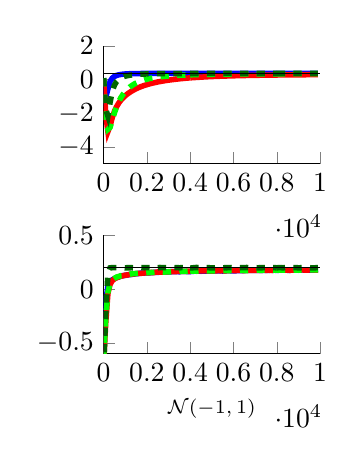
\begin{tikzpicture}
\begin{axis}[%
width=2.75cm,
height=1.5cm,
at={(0\figurewidth,0.591\figureheight)},
scale only axis,
xmin=0,
xmax=10000,
xlabel style={at={(0.5, -0.3)},font=\scriptsize},
xlabel={$\mathcal{N}(-1, 1)$},
ymin=-0.6,
ymax=0.5,
axis background/.style={fill=white},
axis x line*=bottom,
axis y line*=left,
%legend style={at={(0.97,0.03)},anchor=south east,font=\tiny,legend cell align=left,align=left,draw=white!15!black}
]
\addplot [color=blue,solid,line width=2.0pt,forget plot]
  table[row sep=crcr]{%
1	-0.637719551015291\\
101	-0.115098341468071\\
201	0.0267566750476014\\
301	0.0675869352640123\\
401	0.0866333246952596\\
501	0.0983115239330904\\
601	0.108308427838481\\
701	0.113866409318406\\
801	0.122534221245105\\
901	0.126376890278815\\
1001	0.128374434506642\\
1101	0.132646974600422\\
1201	0.135799204027897\\
1301	0.137311239558647\\
1401	0.140304817214583\\
1501	0.143884218294386\\
1601	0.145648529033532\\
1701	0.148818411043197\\
1801	0.149421407844993\\
1901	0.150975770633114\\
2001	0.152869371707057\\
2101	0.152634039505271\\
2201	0.153348184984084\\
2301	0.15556673745373\\
2401	0.15551345731299\\
2501	0.155838160805195\\
2601	0.159089611758047\\
2701	0.158123667172719\\
2801	0.16035186787038\\
2901	0.160525920427632\\
3001	0.160833285872835\\
3101	0.161916646191598\\
3201	0.163099180206922\\
3301	0.163994732406126\\
3401	0.163950187150046\\
3501	0.161837773495146\\
3601	0.165789119412278\\
3701	0.164821371516383\\
3801	0.164929828898244\\
3901	0.164190475227053\\
4001	0.164659026859099\\
};
\addplot [color=blue,solid,line width=2.0pt,forget plot]
  table[row sep=crcr]{%
4001	0.164659026859099\\
4101	0.164831471993002\\
4201	0.168151316446927\\
4301	0.168744727040189\\
4401	0.167682525657707\\
4501	0.166976102732703\\
4601	0.167759435325283\\
4701	0.167232271223769\\
4801	0.168954827223593\\
4901	0.168951835767746\\
5001	0.168298211256784\\
5101	0.169239399728414\\
5201	0.170440548364242\\
5301	0.1708555075236\\
5401	0.170497169493514\\
5501	0.169083433183085\\
5601	0.170822740459134\\
5701	0.171929109044159\\
5801	0.171935885653345\\
5901	0.17145097536683\\
6001	0.171018665380767\\
6101	0.171466662364697\\
6201	0.172315047336064\\
6301	0.17310654798026\\
6401	0.173414987954616\\
6501	0.174096806332626\\
6601	0.175701838634017\\
6701	0.174692055324787\\
6801	0.174685041754456\\
6901	0.174958663777718\\
7001	0.174411272268762\\
7101	0.174096406338874\\
7201	0.174839949338258\\
7301	0.17437553605737\\
7401	0.175784649263438\\
7501	0.175493182581833\\
7601	0.175342904024477\\
7701	0.176906698275076\\
7801	0.176132491198555\\
7901	0.176820591951192\\
8001	0.174737653309965\\
};
\addplot [color=blue,solid,line width=2.0pt]
  table[row sep=crcr]{%
8001	0.174737653309965\\
8101	0.176611932108294\\
8201	0.176787339954467\\
8301	0.177467479527629\\
8401	0.177760836599036\\
8501	0.176052545306522\\
8601	0.175688801226444\\
8701	0.178441773439715\\
8801	0.177745320241462\\
8901	0.177613375823998\\
9001	0.176429980765536\\
9101	0.178211595127866\\
9201	0.179068414898482\\
9301	0.177332573212148\\
9401	0.178968552414107\\
9501	0.178303373655497\\
9601	0.177862455487506\\
9701	0.177473441704438\\
9801	0.178371302679247\\
9901	0.180005264030451\\
};
%\addlegendentry{Q-Learning};
\addplot [color=red,solid,line width=2.0pt,forget plot]
  table[row sep=crcr]{%
1	-0.698391212146146\\
101	-0.309627566079891\\
201	-0.040287198708668\\
301	0.0445734331396394\\
401	0.0782652564255537\\
501	0.0963129325781485\\
601	0.106195531232335\\
701	0.113115501361927\\
801	0.120401664103072\\
901	0.124811390047733\\
1001	0.130905580802179\\
1101	0.132224907856745\\
1201	0.136887731565123\\
1301	0.138904089820326\\
1401	0.14313775188593\\
1501	0.144443664850734\\
1601	0.146886178031267\\
1701	0.147346186696398\\
1801	0.148956040954274\\
1901	0.151127119982039\\
2001	0.152528473605102\\
2101	0.153033563892701\\
2201	0.155921955698901\\
2301	0.154108068770948\\
2401	0.157211307547399\\
2501	0.160312887416608\\
2601	0.15796841499852\\
2701	0.159701410301386\\
2801	0.160838799680524\\
2901	0.161086130482169\\
3001	0.162477233313872\\
3101	0.162723356396651\\
3201	0.163680376160827\\
3301	0.163574293415748\\
3401	0.165026101384654\\
3501	0.166778909152051\\
3601	0.165530402112891\\
3701	0.165281662548759\\
3801	0.165838402716658\\
3901	0.167118442352882\\
4001	0.166526103734004\\
};
\addplot [color=red,solid,line width=2.0pt,forget plot]
  table[row sep=crcr]{%
4001	0.166526103734004\\
4101	0.168912094411004\\
4201	0.168430934666239\\
4301	0.166881411607454\\
4401	0.170085264450872\\
4501	0.169710350372084\\
4601	0.16988155942048\\
4701	0.172529042432877\\
4801	0.169938261077825\\
4901	0.17076898827859\\
5001	0.168548583503673\\
5101	0.171542994975864\\
5201	0.171082663761174\\
5301	0.172263274745613\\
5401	0.17135534609668\\
5501	0.172257150311676\\
5601	0.169303287455057\\
5701	0.172409393338967\\
5801	0.173385403608622\\
5901	0.17572860171652\\
6001	0.173476087926202\\
6101	0.173473627851191\\
6201	0.174682994308827\\
6301	0.175235110283354\\
6401	0.173883546223985\\
6501	0.173345436755732\\
6601	0.174770142507655\\
6701	0.174107726236328\\
6801	0.174789524087105\\
6901	0.17545547280981\\
7001	0.175928407161093\\
7101	0.175386042766137\\
7201	0.176259496218804\\
7301	0.175114776399624\\
7401	0.177404685131434\\
7501	0.175415574067921\\
7601	0.176860080407632\\
7701	0.175531953334793\\
7801	0.17632699047193\\
7901	0.176597679524038\\
8001	0.177183844497557\\
};
\addplot [color=red,solid,line width=2.0pt]
  table[row sep=crcr]{%
8001	0.177183844497557\\
8101	0.176609593316424\\
8201	0.178902256851882\\
8301	0.178083402982601\\
8401	0.17764059495674\\
8501	0.178374745275092\\
8601	0.175874469588634\\
8701	0.177436507243703\\
8801	0.17777482222177\\
8901	0.177907045703159\\
9001	0.178937353663358\\
9101	0.178618877528927\\
9201	0.179038388583844\\
9301	0.177826156384698\\
9401	0.177792835358807\\
9501	0.178958633960206\\
9601	0.179571389128171\\
9701	0.179069847235588\\
9801	0.177704994015177\\
9901	0.179006092242597\\
};
%\addlegendentry{Double Q-Learning};
\addplot [color=green,dashed,line width=2.0pt,forget plot]
  table[row sep=crcr]{%
1	-0.657458201696629\\
101	-0.26552367941705\\
201	-0.0273916865119995\\
301	0.0556525083321782\\
401	0.0867127473000831\\
501	0.100740379112729\\
601	0.112747113302009\\
701	0.118558467801167\\
801	0.125147505983704\\
901	0.126754964729383\\
1001	0.133795901631474\\
1101	0.13626103539402\\
1201	0.138220363467809\\
1301	0.143402195315215\\
1401	0.144322159691306\\
1501	0.14617375804546\\
1601	0.148215704562436\\
1701	0.148604570945089\\
1801	0.148967395849366\\
1901	0.150980751356879\\
2001	0.15277864859661\\
2101	0.153963347157154\\
2201	0.155205518181004\\
2301	0.157023248939876\\
2401	0.157946485715848\\
2501	0.159269433650535\\
2601	0.159158940329338\\
2701	0.160633623530389\\
2801	0.159509630959055\\
2901	0.160991886434804\\
3001	0.161501711727098\\
3101	0.162283565715976\\
3201	0.163910053412234\\
3301	0.163407695334064\\
3401	0.162667798029322\\
3501	0.161829489495098\\
3601	0.16688799757997\\
3701	0.166549726504805\\
3801	0.166552024130298\\
3901	0.168112643256054\\
4001	0.168305726350538\\
};
\addplot [color=green,dashed,line width=2.0pt,forget plot]
  table[row sep=crcr]{%
4001	0.168305726350538\\
4101	0.169158762357662\\
4201	0.168377868518019\\
4301	0.16751910700022\\
4401	0.167884295714342\\
4501	0.168737133329679\\
4601	0.169363376502465\\
4701	0.170702195465595\\
4801	0.170138500009909\\
4901	0.17104506142137\\
5001	0.171213142914739\\
5101	0.171171542444596\\
5201	0.17222960388336\\
5301	0.172134242540051\\
5401	0.170955860951814\\
5501	0.172681176818603\\
5601	0.172304080622426\\
5701	0.172108183513496\\
5801	0.172991312180592\\
5901	0.174174383189575\\
6001	0.17303393958262\\
6101	0.174499278753031\\
6201	0.172330389229239\\
6301	0.174079476141492\\
6401	0.176579318213512\\
6501	0.173840129780774\\
6601	0.173306971655077\\
6701	0.173689151665577\\
6801	0.174845524658897\\
6901	0.175380917827558\\
7001	0.176197036688556\\
7101	0.178209244676661\\
7201	0.176082505559566\\
7301	0.175656530509949\\
7401	0.177800493621152\\
7501	0.175974943498242\\
7601	0.176148668283351\\
7701	0.177624860066028\\
7801	0.175754637074485\\
7901	0.176883840525308\\
8001	0.177289382035878\\
};
\addplot [color=green,dashed,line width=2.0pt]
  table[row sep=crcr]{%
8001	0.177289382035878\\
8101	0.17746761555893\\
8201	0.17913347516714\\
8301	0.176906650074134\\
8401	0.176544087515426\\
8501	0.177416138262302\\
8601	0.177316971590698\\
8701	0.176058907304505\\
8801	0.178340069219635\\
8901	0.177372597043487\\
9001	0.178264856448831\\
9101	0.178661142428752\\
9201	0.178289834948021\\
9301	0.18031757182638\\
9401	0.177643031414879\\
9501	0.178086764195182\\
9601	0.180643690668999\\
9701	0.179351624364642\\
9801	0.179389018277428\\
9901	0.180088888801303\\
};
%\addlegendentry{W Q-Learning};
\addplot [color=black!60!green,dashed,line width=2.0pt,forget plot]
  table[row sep=crcr]{%
1	-0.743196272765407\\
101	-0.22734395467778\\
201	0.141355374617717\\
301	0.198277678679742\\
401	0.201057652506112\\
501	0.199974850142352\\
601	0.20046236466506\\
701	0.198569709815126\\
801	0.201105685513219\\
901	0.200792170946353\\
1001	0.199008311998773\\
1101	0.199624366257011\\
1201	0.19950540373125\\
1301	0.199741430678898\\
1401	0.198671923501484\\
1501	0.200072798486755\\
1601	0.200043418609058\\
1701	0.201250697298922\\
1801	0.200842488308673\\
1901	0.19961119838491\\
2001	0.200127791634921\\
2101	0.201007352465115\\
2201	0.200045528176068\\
2301	0.201230521973999\\
2401	0.199005357948586\\
2501	0.199171532140862\\
2601	0.201841657570358\\
2701	0.200597675163225\\
2801	0.20064160189569\\
2901	0.199967906708768\\
3001	0.200356821959047\\
3101	0.200114359745857\\
3201	0.201460379934638\\
3301	0.200873380029545\\
3401	0.20123197190204\\
3501	0.198618060729608\\
3601	0.201262038143238\\
3701	0.199189422139898\\
3801	0.20093255078962\\
3901	0.199891883148731\\
4001	0.199050216694974\\
};
\addplot [color=black!60!green,dashed,line width=2.0pt,forget plot]
  table[row sep=crcr]{%
4001	0.199050216694974\\
4101	0.19850759627998\\
4201	0.201210652634483\\
4301	0.202083313391532\\
4401	0.199988512792708\\
4501	0.199095842417111\\
4601	0.199342054973802\\
4701	0.19877219735328\\
4801	0.20012874623\\
4901	0.199341624189105\\
5001	0.197963559365639\\
5101	0.198324208959588\\
5201	0.199184817330324\\
5301	0.199569431148287\\
5401	0.199931867571548\\
5501	0.198193289128128\\
5601	0.199745542343116\\
5701	0.199376884850851\\
5801	0.201390196510478\\
5901	0.199966213695568\\
6001	0.198942737123522\\
6101	0.198792437691014\\
6201	0.199680891640625\\
6301	0.19963711757799\\
6401	0.200939507917258\\
6501	0.200397557273177\\
6601	0.201840743098999\\
6701	0.201222904008298\\
6801	0.20059302208094\\
6901	0.20084642412873\\
7001	0.200464562466123\\
7101	0.198875120103301\\
7201	0.199626160819755\\
7301	0.199367178716152\\
7401	0.200156127462517\\
7501	0.200114826270743\\
7601	0.20041465805781\\
7701	0.19954596448865\\
7801	0.200496480031321\\
7901	0.200115777757787\\
8001	0.199043299471687\\
};
\addplot [color=black!60!green,dashed,line width=2.0pt]
  table[row sep=crcr]{%
8001	0.199043299471687\\
8101	0.200052237763624\\
8201	0.199754104361046\\
8301	0.199112659839813\\
8401	0.201157329452716\\
8501	0.199755313324812\\
8601	0.198983262964664\\
8701	0.199833351145233\\
8801	0.200280576597993\\
8901	0.199824734602472\\
9001	0.199178054645492\\
9101	0.199417183755105\\
9201	0.200701080945557\\
9301	0.198717227629253\\
9401	0.199132490617428\\
9501	0.200708744833029\\
9601	0.198360914260952\\
9701	0.198831456764817\\
9801	0.19947434487363\\
9901	0.200970106243487\\
};
%\addlegendentry{W Q-Learning with W-policy};

\addplot [color=black,solid,forget plot]
  table[row sep=crcr]{%
0	0.2\\
10000	0.2\\
};

\end{axis}
\begin{axis}[%
width=2.75cm,
height=1.5cm,
at={(0\figurewidth,0\figureheight)},
scale only axis,
%xlabel={Number of Steps},
xmin=0,
xmax=10000,
ymin=-5,
ymax=2,
axis background/.style={fill=white},
axis x line*=bottom,
axis y line*=left,
%legend style={legend cell align=left,align=left,draw=white!15!black}
]
\addplot [color=blue,solid,line width=2.0pt,forget plot]
  table[row sep=crcr]{%
1	0.0826247151089759\\
101	-1.06472770393013\\
201	-0.551155091617003\\
301	-0.116195705263244\\
401	0.0842423074320162\\
501	0.185085209302771\\
601	0.244671956241388\\
701	0.281366265165336\\
801	0.303187256126485\\
901	0.320634742086047\\
1001	0.331333276945184\\
1101	0.339060110793764\\
1201	0.344756661810358\\
1301	0.348337650720523\\
1401	0.35155971281478\\
1501	0.35324532445827\\
1601	0.35590581185715\\
1701	0.357939528677409\\
1801	0.360312232734291\\
1901	0.361473851779349\\
2001	0.362155909378586\\
2101	0.362869456500928\\
2201	0.36338934323476\\
2301	0.364472148337704\\
2401	0.365180357084457\\
2501	0.365559408760726\\
2601	0.365780732266266\\
2701	0.366611354719254\\
2801	0.366916264343977\\
2901	0.36745938670539\\
3001	0.367891797434317\\
3101	0.367873739141163\\
3201	0.367879499733971\\
3301	0.368934055255745\\
3401	0.368824343282057\\
3501	0.368579897893469\\
3601	0.368282903145517\\
3701	0.368634041593039\\
3801	0.368621297251302\\
3901	0.369079258511253\\
4001	0.36872692268159\\
};
\addplot [color=blue,solid,line width=2.0pt,forget plot]
  table[row sep=crcr]{%
4001	0.36872692268159\\
4101	0.36811735327801\\
4201	0.368170960745074\\
4301	0.368029761574498\\
4401	0.36817161065168\\
4501	0.368319794975271\\
4601	0.368336732484551\\
4701	0.368271782781747\\
4801	0.368082885956699\\
4901	0.368136065940824\\
5001	0.368206459206751\\
5101	0.368156209716088\\
5201	0.368041706995451\\
5301	0.368069037327376\\
5401	0.367899480154021\\
5501	0.367626478144674\\
5601	0.367520909960016\\
5701	0.367599729808008\\
5801	0.367880974147272\\
5901	0.368065100765461\\
6001	0.367594449772787\\
6101	0.367415119750296\\
6201	0.367487874542961\\
6301	0.367575363475594\\
6401	0.367989791146562\\
6501	0.367742459740795\\
6601	0.367847258568896\\
6701	0.36805242093763\\
6801	0.367902097642318\\
6901	0.36806157914497\\
7001	0.36821734269063\\
7101	0.367857130247379\\
7201	0.367704848998586\\
7301	0.367685762473084\\
7401	0.367465545038496\\
7501	0.36759888621404\\
7601	0.367469245664592\\
7701	0.367434803733257\\
7801	0.367648020987915\\
7901	0.367553833960486\\
8001	0.367669550915278\\
};
\addplot [color=blue,solid,line width=2.0pt]
  table[row sep=crcr]{%
8001	0.367669550915278\\
8101	0.367576373492418\\
8201	0.367298249033594\\
8301	0.367490275125471\\
8401	0.367632326598567\\
8501	0.367646613953404\\
8601	0.367889284102747\\
8701	0.367642473836057\\
8801	0.367630915648112\\
8901	0.367793284377107\\
9001	0.367566546575047\\
9101	0.36729085310594\\
9201	0.367194634768844\\
9301	0.367237118883458\\
9401	0.367198276849467\\
9501	0.367088894686834\\
9601	0.366925442469374\\
9701	0.3668036135164\\
9801	0.366594486461351\\
9901	0.366345943058066\\
};
%%\addlegendentry{Q-Learning};
\addplot [color=red,solid,line width=2.0pt,forget plot]
  table[row sep=crcr]{%
1	0.0438481769819867\\
101	-2.05683265510824\\
201	-3.08135887090524\\
301	-2.74878164779622\\
401	-2.25867930714192\\
501	-1.88480326832686\\
601	-1.60735166558846\\
701	-1.39239179119975\\
801	-1.22070712298519\\
901	-1.07957893353263\\
1001	-0.960154880360175\\
1101	-0.8556526310952\\
1201	-0.763935252741822\\
1301	-0.682222339091102\\
1401	-0.609859484494813\\
1501	-0.543417364416149\\
1601	-0.485604661144311\\
1701	-0.433055639883692\\
1801	-0.385361765258493\\
1901	-0.34108199850394\\
2001	-0.301478956704579\\
2101	-0.263929448416628\\
2201	-0.230268340845077\\
2301	-0.198560053080104\\
2401	-0.170107198545453\\
2501	-0.143117168580839\\
2601	-0.11778973442818\\
2701	-0.0949693416302268\\
2801	-0.0732966852011464\\
2901	-0.0531575471728307\\
3001	-0.0345709940099992\\
3101	-0.0169566464583421\\
3201	-0.000620864476868604\\
3301	0.0152489272893812\\
3401	0.0302320731459778\\
3501	0.0436755643042771\\
3601	0.056460964432852\\
3701	0.068537531924695\\
3801	0.080173609184005\\
3901	0.0910281373078906\\
4001	0.101183166389268\\
};
\addplot [color=red,solid,line width=2.0pt,forget plot]
  table[row sep=crcr]{%
4001	0.101183166389268\\
4101	0.110448220886838\\
4201	0.119573083811334\\
4301	0.128174041732676\\
4401	0.136032177760223\\
4501	0.143995291715286\\
4601	0.151535460753634\\
4701	0.158709928226806\\
4801	0.165868930634399\\
4901	0.1726162361276\\
5001	0.178437110394564\\
5101	0.18362020897032\\
5201	0.188971279637232\\
5301	0.194164890753102\\
5401	0.199159084726044\\
5501	0.203622186258216\\
5601	0.208053923487869\\
5701	0.211921595194456\\
5801	0.216135972758063\\
5901	0.220161651143656\\
6001	0.223961116181807\\
6101	0.227487342334993\\
6201	0.23082583685821\\
6301	0.234029757566999\\
6401	0.237154670494895\\
6501	0.239999474177544\\
6601	0.242670831868438\\
6701	0.245310727025612\\
6801	0.247772269472855\\
6901	0.250068187981391\\
7001	0.252334110965566\\
7101	0.254560011718836\\
7201	0.256599154791444\\
7301	0.258959452287645\\
7401	0.260885492849696\\
7501	0.262955860050809\\
7601	0.264527247466345\\
7701	0.266265985863675\\
7801	0.26781025895691\\
7901	0.269482670255599\\
8001	0.271013946329352\\
};
\addplot [color=red,solid,line width=2.0pt]
  table[row sep=crcr]{%
8001	0.271013946329352\\
8101	0.272124301914794\\
8201	0.273376246240044\\
8301	0.274677588148513\\
8401	0.276050598825301\\
8501	0.277269956320838\\
8601	0.278352293287244\\
8701	0.279441569588469\\
8801	0.280576124094505\\
8901	0.281806409726864\\
9001	0.282799053832534\\
9101	0.283858013200804\\
9201	0.284795559917676\\
9301	0.285801598572903\\
9401	0.286686218374622\\
9501	0.287581336046537\\
9601	0.288398087657342\\
9701	0.289399678172091\\
9801	0.290047721518298\\
9901	0.290650112054829\\
};
%%\addlegendentry{Double Q-Learning};
\addplot [color=green,dashed,line width=2.0pt,forget plot]
  table[row sep=crcr]{%
1	0.0863233285703327\\
101	-2.23636366430177\\
201	-2.94813954203173\\
301	-2.83343913648129\\
401	-2.41125393205922\\
501	-1.97725097270727\\
601	-1.61194068037334\\
701	-1.31256412724501\\
801	-1.06876635881666\\
901	-0.870318387430078\\
1001	-0.7076731944166\\
1101	-0.570247888499741\\
1201	-0.456250599264968\\
1301	-0.360679784706704\\
1401	-0.278474959966871\\
1501	-0.208501342014716\\
1601	-0.148930760193503\\
1701	-0.0969885644657972\\
1801	-0.0522530185934204\\
1901	-0.0133476822102435\\
2001	0.0210345335707575\\
2101	0.0515382906592238\\
2201	0.0785340375039641\\
2301	0.101932823856247\\
2401	0.123658432591493\\
2501	0.142344988408544\\
2601	0.15923509378122\\
2701	0.174150652848542\\
2801	0.188115905399324\\
2901	0.200940793735123\\
3001	0.212021397089136\\
3101	0.222059259668345\\
3201	0.231087355141758\\
3301	0.240128627946129\\
3401	0.247995819788922\\
3501	0.254881528908461\\
3601	0.260946932717882\\
3701	0.267051651275721\\
3801	0.272433135819769\\
3901	0.277495108404551\\
4001	0.282379893116693\\
};
\addplot [color=green,dashed,line width=2.0pt,forget plot]
  table[row sep=crcr]{%
4001	0.282379893116693\\
4101	0.286730818189707\\
4201	0.290611759910284\\
4301	0.294418426937649\\
4401	0.297889989945718\\
4501	0.30108009949022\\
4601	0.304176295753289\\
4701	0.307104675689879\\
4801	0.309713760930909\\
4901	0.31219502777504\\
5001	0.31481555680983\\
5101	0.317022827566463\\
5201	0.318804063916133\\
5301	0.320706165441194\\
5401	0.322463518633029\\
5501	0.324237245300882\\
5601	0.325642226631901\\
5701	0.32699497047543\\
5801	0.328161697767099\\
5901	0.329372463957587\\
6001	0.330626614420265\\
6101	0.331425073183482\\
6201	0.332572100836635\\
6301	0.333333879986821\\
6401	0.334360143185149\\
6501	0.335206344494929\\
6601	0.335886561340282\\
6701	0.336462440273006\\
6801	0.337098589676067\\
6901	0.337721146183107\\
7001	0.338329713440309\\
7101	0.338971178645732\\
7201	0.339671635371608\\
7301	0.340428680477876\\
7401	0.34100526578709\\
7501	0.341576938543794\\
7601	0.342084959376394\\
7701	0.342383618859889\\
7801	0.342942666998469\\
7901	0.343216894245941\\
8001	0.34334489257734\\
};
\addplot [color=green,dashed,line width=2.0pt]
  table[row sep=crcr]{%
8001	0.34334489257734\\
8101	0.343836815123299\\
8201	0.34414202861494\\
8301	0.344570958113725\\
8401	0.344735304240098\\
8501	0.345049647634513\\
8601	0.345526679653349\\
8701	0.345572337143374\\
8801	0.345668822871783\\
8901	0.345953058064021\\
9001	0.346262898376542\\
9101	0.346493006854678\\
9201	0.346811211861939\\
9301	0.346975566450926\\
9401	0.347224179064551\\
9501	0.347085560791696\\
9601	0.347074262099001\\
9701	0.347266307587063\\
9801	0.34734769331109\\
9901	0.347411249249158\\
};
%%\addlegendentry{Weighted Q-Learning};
\addplot [color=black!60!green,dashed,line width=2.0pt,forget plot]
  table[row sep=crcr]{%
1	0.0826247151089759\\
101	-1.76246578487334\\
201	-2.159532491534\\
301	-1.35280605710655\\
401	-0.695300487787006\\
501	-0.328877619920979\\
601	-0.118378358331514\\
701	0.0125254785679825\\
801	0.0978995796222427\\
901	0.158958835519288\\
1001	0.201819871527414\\
1101	0.232224175283838\\
1201	0.256138776242095\\
1301	0.275165086895694\\
1401	0.289086016422739\\
1501	0.299700433336386\\
1601	0.309052293239382\\
1701	0.316774486907511\\
1801	0.322972467752642\\
1901	0.328425174035398\\
2001	0.332968262876152\\
2101	0.336834370032047\\
2201	0.340174962100695\\
2301	0.3433011367475\\
2401	0.345309454480614\\
2501	0.346970864224801\\
2601	0.348656637613027\\
2701	0.35053740842368\\
2801	0.351771654413938\\
2901	0.353376174705683\\
3001	0.354343588328915\\
3101	0.355089370437323\\
3201	0.355824926492844\\
3301	0.356312978893104\\
3401	0.357180255566312\\
3501	0.357724261028761\\
3601	0.357940860417476\\
3701	0.359015278820603\\
3801	0.358973808157919\\
3901	0.359333388646266\\
4001	0.359686197617507\\
};
\addplot [color=black!60!green,dashed,line width=2.0pt,forget plot]
  table[row sep=crcr]{%
4001	0.359686197617507\\
4101	0.359837853619222\\
4201	0.359781396361014\\
4301	0.360093922523345\\
4401	0.360516659682925\\
4501	0.360889583731495\\
4601	0.361038138061544\\
4701	0.361263632195548\\
4801	0.361391987237487\\
4901	0.361443382183481\\
5001	0.361239740252446\\
5101	0.361101440896913\\
5201	0.361014527021096\\
5301	0.360870563648688\\
5401	0.360930988083647\\
5501	0.360889874666625\\
5601	0.361064722993889\\
5701	0.36104618892159\\
5801	0.3613377102518\\
5901	0.36162117788521\\
6001	0.361609237428172\\
6101	0.361781551375296\\
6201	0.361916500415615\\
6301	0.361805032784444\\
6401	0.361744256747537\\
6501	0.361666343607329\\
6601	0.361549340556104\\
6701	0.361621852302723\\
6801	0.361794722339838\\
6901	0.362052644171754\\
7001	0.362169970216568\\
7101	0.36224791742527\\
7201	0.362280004475481\\
7301	0.362361431418091\\
7401	0.362268262043905\\
7501	0.362446122851253\\
7601	0.362335321827825\\
7701	0.362236601172655\\
7801	0.362360199486375\\
7901	0.362390417599617\\
8001	0.362311102294251\\
};
\addplot [color=black!60!green,dashed,line width=2.0pt]
  table[row sep=crcr]{%
8001	0.362311102294251\\
8101	0.362181187140345\\
8201	0.36213759294929\\
8301	0.362132002496544\\
8401	0.361976402483073\\
8501	0.362140398893135\\
8601	0.362069347285534\\
8701	0.362203888619867\\
8801	0.362122398025186\\
8901	0.361938069053733\\
9001	0.361920256487379\\
9101	0.361862354097609\\
9201	0.361894059420208\\
9301	0.361939572340069\\
9401	0.361928441172321\\
9501	0.362019189113419\\
9601	0.3621012085692\\
9701	0.361943460523865\\
9801	0.361736519518131\\
9901	0.361721314534279\\
};
%%\addlegendentry{W Q-Learning with W-policy};

\addplot [color=black,solid,forget plot]
  table[row sep=crcr]{%
0	0.36\\
10000	0.36\\
};

\end{axis}
\end{tikzpicture}%


 \centering \textbf{Forex}\\
   \vspace{.1cm}
   % This file was created by matlab2tikz.
%
%The latest updates can be retrieved from
%  http://www.mathworks.com/matlabcentral/fileexchange/22022-matlab2tikz-matlab2tikz
%where you can also make suggestions and rate matlab2tikz.
%
\definecolor{mycolor1}{rgb}{0.55000,0.73000,0.55000}%
%
\begin{tikzpicture}

\begin{axis}[%
width=4cm,
height=3cm,
at={(0\figurewidth,0\figureheight)},
scale only axis,
xmin=0,
xmax=30,
xlabel={\#training episodes},
%x label style={at={(1.5, -0.5)}},
ymin=-4,
ymax=16,
ytick={-4,-2,0,2,4,6,8,10,12,14,16},
yticklabels={{-4\%},{-2\%},{ 0\%},{ 2\%},{ 4\%},{ 6\%},{ 8\%},{10\%},{12\%},{14\%},{16\%}},
ylabel={Profit per year},
axis background/.style={fill=white},
axis x line*=bottom,
axis y line*=left,
%legend style={at={(1.75,0.05)},anchor=south east,font=\tiny,legend cell align=left,align=left,draw=white!15!black}
]

\addplot[area legend,solid,fill=blue,fill opacity=0.15,forget plot]
table[row sep=crcr] {%
x	y\\
1	-3.15693460148593\\
2	-0.0211141029694804\\
3	2.22760417772162\\
4	4.3384301594235\\
5	5.22035111055205\\
6	6.30250058543432\\
7	7.07399969913459\\
8	8.75542296472648\\
9	8.5001665363165\\
10	9.4211566083579\\
11	10.0493823093585\\
12	10.2277158578188\\
13	10.9434768579821\\
14	10.8548957334046\\
15	11.8703703906568\\
16	11.7852689360159\\
17	11.9499585839813\\
18	12.3248830397154\\
19	12.2494729801999\\
20	12.62282058892\\
21	12.9717898370172\\
22	13.6109258816276\\
23	13.4166887351071\\
24	13.6833506289404\\
25	13.5715333887657\\
26	13.6794217048174\\
27	13.7778088205844\\
28	13.854727384806\\
29	13.9748783746367\\
30	14.1387713574584\\
30	15.554561975875\\
29	15.47268829203\\
28	15.119372615194\\
27	15.136024512749\\
26	15.1699449618493\\
25	14.9709999445676\\
24	14.9751160377262\\
23	14.9061112648929\\
22	15.0625074517057\\
21	14.3777101629828\\
20	14.0269460777466\\
19	13.8147603531335\\
18	13.8704836269513\\
17	13.411274749352\\
16	13.1891310639841\\
15	13.3116962760099\\
14	12.4080042665954\\
13	12.3618898086846\\
12	11.7784841421812\\
11	11.5638843573081\\
10	10.8888433916421\\
9	10.0848001303502\\
8	9.99601036860686\\
7	8.78303363419875\\
6	7.96906608123235\\
5	6.90848222278129\\
4	6.06940317390983\\
3	4.05126248894504\\
2	1.83254743630281\\
1	-1.17406539851407\\
}--cycle;
\addplot [color=white!55!blue,solid,forget plot]
  table[row sep=crcr]{%
1	-3.15693460148593\\
2	-0.0211141029694804\\
3	2.22760417772162\\
4	4.3384301594235\\
5	5.22035111055205\\
6	6.30250058543432\\
7	7.07399969913459\\
8	8.75542296472648\\
9	8.5001665363165\\
10	9.4211566083579\\
11	10.0493823093585\\
12	10.2277158578188\\
13	10.9434768579821\\
14	10.8548957334046\\
15	11.8703703906568\\
16	11.7852689360159\\
17	11.9499585839813\\
18	12.3248830397154\\
19	12.2494729801999\\
20	12.62282058892\\
21	12.9717898370172\\
22	13.6109258816276\\
23	13.4166887351071\\
24	13.6833506289404\\
25	13.5715333887657\\
26	13.6794217048174\\
27	13.7778088205844\\
28	13.854727384806\\
29	13.9748783746367\\
30	14.1387713574584\\
};
\addplot [color=white!55!blue,solid,forget plot]
  table[row sep=crcr]{%
1	-1.17406539851407\\
2	1.83254743630281\\
3	4.05126248894504\\
4	6.06940317390983\\
5	6.90848222278129\\
6	7.96906608123235\\
7	8.78303363419875\\
8	9.99601036860686\\
9	10.0848001303502\\
10	10.8888433916421\\
11	11.5638843573081\\
12	11.7784841421812\\
13	12.3618898086846\\
14	12.4080042665954\\
15	13.3116962760099\\
16	13.1891310639841\\
17	13.411274749352\\
18	13.8704836269513\\
19	13.8147603531335\\
20	14.0269460777466\\
21	14.3777101629828\\
22	15.0625074517057\\
23	14.9061112648929\\
24	14.9751160377262\\
25	14.9709999445676\\
26	15.1699449618493\\
27	15.136024512749\\
28	15.119372615194\\
29	15.47268829203\\
30	15.554561975875\\
};
\addplot [color=white!55!blue,dashed,forget plot]
  table[row sep=crcr]{%
1	-3.15693460148593\\
2	-0.0211141029694804\\
3	2.22760417772162\\
4	4.3384301594235\\
5	5.22035111055205\\
6	6.30250058543432\\
7	7.07399969913459\\
8	8.75542296472648\\
9	8.5001665363165\\
10	9.4211566083579\\
11	10.0493823093585\\
12	10.2277158578188\\
13	10.9434768579821\\
14	10.8548957334046\\
15	11.8703703906568\\
16	11.7852689360159\\
17	11.9499585839813\\
18	12.3248830397154\\
19	12.2494729801999\\
20	12.62282058892\\
21	12.9717898370172\\
22	13.6109258816276\\
23	13.4166887351071\\
24	13.6833506289404\\
25	13.5715333887657\\
26	13.6794217048174\\
27	13.7778088205844\\
28	13.854727384806\\
29	13.9748783746367\\
30	14.1387713574584\\
};
\addplot [color=white!55!blue,dashed,forget plot]
  table[row sep=crcr]{%
1	-1.17406539851407\\
2	1.83254743630281\\
3	4.05126248894504\\
4	6.06940317390983\\
5	6.90848222278129\\
6	7.96906608123235\\
7	8.78303363419875\\
8	9.99601036860686\\
9	10.0848001303502\\
10	10.8888433916421\\
11	11.5638843573081\\
12	11.7784841421812\\
13	12.3618898086846\\
14	12.4080042665954\\
15	13.3116962760099\\
16	13.1891310639841\\
17	13.411274749352\\
18	13.8704836269513\\
19	13.8147603531335\\
20	14.0269460777466\\
21	14.3777101629828\\
22	15.0625074517057\\
23	14.9061112648929\\
24	14.9751160377262\\
25	14.9709999445676\\
26	15.1699449618493\\
27	15.136024512749\\
28	15.119372615194\\
29	15.47268829203\\
30	15.554561975875\\
};
\addplot [color=blue,solid,line width=2.0pt]
  table[row sep=crcr]{%
1	-2.1655\\
2	0.905716666666667\\
3	3.13943333333333\\
4	5.20391666666667\\
5	6.06441666666667\\
6	7.13578333333333\\
7	7.92851666666667\\
8	9.37571666666667\\
9	9.29248333333333\\
10	10.155\\
11	10.8066333333333\\
12	11.0031\\
13	11.6526833333333\\
14	11.63145\\
15	12.5910333333333\\
16	12.4872\\
17	12.6806166666667\\
18	13.0976833333333\\
19	13.0321166666667\\
20	13.3248833333333\\
21	13.67475\\
22	14.3367166666667\\
23	14.1614\\
24	14.3292333333333\\
25	14.2712666666667\\
26	14.4246833333333\\
27	14.4569166666667\\
28	14.48705\\
29	14.7237833333333\\
30	14.8466666666667\\
};
%\addlegendentry{QL};

\addplot[area legend,solid,fill=red,fill opacity=0.15,forget plot]
table[row sep=crcr] {%
x	y\\
1	-3.77675681118774\\
2	-1.29038297219904\\
3	0.595213108302517\\
4	2.14111458105885\\
5	3.43758742417323\\
6	4.56812279762849\\
7	4.94464187682489\\
8	6.00703811614902\\
9	5.97350376498831\\
10	6.13152899521185\\
11	6.86820263351419\\
12	7.03673398465404\\
13	7.46045001282118\\
14	7.6647219355733\\
15	8.14621260406598\\
16	8.6454011809304\\
17	8.52391302882667\\
18	8.50071475856892\\
19	9.09390875395839\\
20	8.51446464073529\\
21	8.92133558915563\\
22	9.07834747631174\\
23	9.41047221900825\\
24	9.54128107479261\\
25	9.58620778108908\\
26	9.49434013114662\\
27	9.48085609126858\\
28	9.90469797270944\\
29	10.1105524522526\\
30	9.77733358101079\\
30	10.8619664189892\\
29	11.3052142144141\\
28	10.9336686939572\\
27	10.6723772420647\\
26	10.5122598688534\\
25	10.7922922189109\\
24	10.7742189252074\\
23	10.4685611143251\\
22	10.4528191903549\\
21	10.1880977441777\\
20	9.68126869259804\\
19	10.2222912460416\\
18	9.68891857476442\\
17	9.78335363784\\
16	9.80486548573627\\
15	9.39198739593403\\
14	8.89251139776003\\
13	8.84594998717882\\
12	8.45793268201263\\
11	8.15429736648581\\
10	7.52087100478815\\
9	7.35946290167836\\
8	7.43396188385098\\
7	6.23452478984178\\
6	5.77224386903817\\
5	4.63927924249344\\
4	3.69695208560782\\
3	2.11485355836415\\
2	0.225882972199042\\
1	-1.78670985547893\\
}--cycle;
\addplot [color=white!55!red,solid,forget plot]
  table[row sep=crcr]{%
1	-3.77675681118774\\
2	-1.29038297219904\\
3	0.595213108302517\\
4	2.14111458105885\\
5	3.43758742417323\\
6	4.56812279762849\\
7	4.94464187682489\\
8	6.00703811614902\\
9	5.97350376498831\\
10	6.13152899521185\\
11	6.86820263351419\\
12	7.03673398465404\\
13	7.46045001282118\\
14	7.6647219355733\\
15	8.14621260406598\\
16	8.6454011809304\\
17	8.52391302882667\\
18	8.50071475856892\\
19	9.09390875395839\\
20	8.51446464073529\\
21	8.92133558915563\\
22	9.07834747631174\\
23	9.41047221900825\\
24	9.54128107479261\\
25	9.58620778108908\\
26	9.49434013114662\\
27	9.48085609126858\\
28	9.90469797270944\\
29	10.1105524522526\\
30	9.77733358101079\\
};
\addplot [color=white!55!red,solid,forget plot]
  table[row sep=crcr]{%
1	-1.78670985547893\\
2	0.225882972199042\\
3	2.11485355836415\\
4	3.69695208560782\\
5	4.63927924249344\\
6	5.77224386903817\\
7	6.23452478984178\\
8	7.43396188385098\\
9	7.35946290167836\\
10	7.52087100478815\\
11	8.15429736648581\\
12	8.45793268201263\\
13	8.84594998717882\\
14	8.89251139776003\\
15	9.39198739593403\\
16	9.80486548573627\\
17	9.78335363784\\
18	9.68891857476442\\
19	10.2222912460416\\
20	9.68126869259804\\
21	10.1880977441777\\
22	10.4528191903549\\
23	10.4685611143251\\
24	10.7742189252074\\
25	10.7922922189109\\
26	10.5122598688534\\
27	10.6723772420647\\
28	10.9336686939572\\
29	11.3052142144141\\
30	10.8619664189892\\
};
\addplot [color=white!55!red,dashed,forget plot]
  table[row sep=crcr]{%
1	-3.77675681118774\\
2	-1.29038297219904\\
3	0.595213108302517\\
4	2.14111458105885\\
5	3.43758742417323\\
6	4.56812279762849\\
7	4.94464187682489\\
8	6.00703811614902\\
9	5.97350376498831\\
10	6.13152899521185\\
11	6.86820263351419\\
12	7.03673398465404\\
13	7.46045001282118\\
14	7.6647219355733\\
15	8.14621260406598\\
16	8.6454011809304\\
17	8.52391302882667\\
18	8.50071475856892\\
19	9.09390875395839\\
20	8.51446464073529\\
21	8.92133558915563\\
22	9.07834747631174\\
23	9.41047221900825\\
24	9.54128107479261\\
25	9.58620778108908\\
26	9.49434013114662\\
27	9.48085609126858\\
28	9.90469797270944\\
29	10.1105524522526\\
30	9.77733358101079\\
};
\addplot [color=white!55!red,dashed,forget plot]
  table[row sep=crcr]{%
1	-1.78670985547893\\
2	0.225882972199042\\
3	2.11485355836415\\
4	3.69695208560782\\
5	4.63927924249344\\
6	5.77224386903817\\
7	6.23452478984178\\
8	7.43396188385098\\
9	7.35946290167836\\
10	7.52087100478815\\
11	8.15429736648581\\
12	8.45793268201263\\
13	8.84594998717882\\
14	8.89251139776003\\
15	9.39198739593403\\
16	9.80486548573627\\
17	9.78335363784\\
18	9.68891857476442\\
19	10.2222912460416\\
20	9.68126869259804\\
21	10.1880977441777\\
22	10.4528191903549\\
23	10.4685611143251\\
24	10.7742189252074\\
25	10.7922922189109\\
26	10.5122598688534\\
27	10.6723772420647\\
28	10.9336686939572\\
29	11.3052142144141\\
30	10.8619664189892\\
};
\addplot [color=red,solid,line width=2.0pt]
  table[row sep=crcr]{%
1	-2.78173333333333\\
2	-0.53225\\
3	1.35503333333333\\
4	2.91903333333333\\
5	4.03843333333333\\
6	5.17018333333333\\
7	5.58958333333333\\
8	6.7205\\
9	6.66648333333333\\
10	6.8262\\
11	7.51125\\
12	7.74733333333333\\
13	8.1532\\
14	8.27861666666666\\
15	8.7691\\
16	9.22513333333334\\
17	9.15363333333334\\
18	9.09481666666667\\
19	9.6581\\
20	9.09786666666667\\
21	9.55471666666667\\
22	9.76558333333334\\
23	9.93951666666667\\
24	10.15775\\
25	10.18925\\
26	10.0033\\
27	10.0766166666667\\
28	10.4191833333333\\
29	10.7078833333333\\
30	10.31965\\
};
%\addlegendentry{DQL};

\addplot[area legend,solid,fill=green,fill opacity=0.15,forget plot]
table[row sep=crcr] {%
x	y\\
1	-1.93038739746516\\
2	0.384749212563258\\
3	1.31691959681039\\
4	3.14285023792131\\
5	4.42123805840447\\
6	4.86399055915682\\
7	5.5408052664472\\
8	6.84783991409324\\
9	7.47985875439275\\
10	8.46278078847247\\
11	8.63810944616976\\
12	9.12410787969795\\
13	9.64542080310242\\
14	9.96803290306442\\
15	10.4804324430149\\
16	10.485825375793\\
17	10.3857207275904\\
18	11.0738329254621\\
19	11.2441580669219\\
20	11.600256481812\\
21	11.7904885847479\\
22	12.0054127055173\\
23	12.2387493684716\\
24	12.3135051522781\\
25	12.6657688580016\\
26	12.5075516414441\\
27	13.180901651516\\
28	12.4163926262136\\
29	13.0036338575172\\
30	13.1254713717597\\
30	14.241495294907\\
29	14.1439661424828\\
28	13.5967407071197\\
27	14.2966316818173\\
26	13.7230150252226\\
25	13.8693644753317\\
24	13.5257948477219\\
23	13.3513172981951\\
22	13.2476539611493\\
21	13.0313114152521\\
20	12.9157101848546\\
19	12.4350419330781\\
18	12.2804004078712\\
17	11.6713126057429\\
16	11.6044079575403\\
15	11.7888342236517\\
14	11.1813337636022\\
13	11.0553791968976\\
12	10.6370587869687\\
11	10.2217572204969\\
10	10.0027192115275\\
9	8.93330791227391\\
8	8.31479341924009\\
7	7.08932806688614\\
6	6.47287610750984\\
5	6.04672860826219\\
4	4.59994976207869\\
3	3.15074706985628\\
2	2.17078412077008\\
1	-0.152579269201507\\
}--cycle;
\addplot [color=white!55!green,solid,forget plot]
  table[row sep=crcr]{%
1	-1.93038739746516\\
2	0.384749212563258\\
3	1.31691959681039\\
4	3.14285023792131\\
5	4.42123805840447\\
6	4.86399055915682\\
7	5.5408052664472\\
8	6.84783991409324\\
9	7.47985875439275\\
10	8.46278078847247\\
11	8.63810944616976\\
12	9.12410787969795\\
13	9.64542080310242\\
14	9.96803290306442\\
15	10.4804324430149\\
16	10.485825375793\\
17	10.3857207275904\\
18	11.0738329254621\\
19	11.2441580669219\\
20	11.600256481812\\
21	11.7904885847479\\
22	12.0054127055173\\
23	12.2387493684716\\
24	12.3135051522781\\
25	12.6657688580016\\
26	12.5075516414441\\
27	13.180901651516\\
28	12.4163926262136\\
29	13.0036338575172\\
30	13.1254713717597\\
};
\addplot [color=white!55!green,solid,forget plot]
  table[row sep=crcr]{%
1	-0.152579269201507\\
2	2.17078412077008\\
3	3.15074706985628\\
4	4.59994976207869\\
5	6.04672860826219\\
6	6.47287610750984\\
7	7.08932806688614\\
8	8.31479341924009\\
9	8.93330791227391\\
10	10.0027192115275\\
11	10.2217572204969\\
12	10.6370587869687\\
13	11.0553791968976\\
14	11.1813337636022\\
15	11.7888342236517\\
16	11.6044079575403\\
17	11.6713126057429\\
18	12.2804004078712\\
19	12.4350419330781\\
20	12.9157101848546\\
21	13.0313114152521\\
22	13.2476539611493\\
23	13.3513172981951\\
24	13.5257948477219\\
25	13.8693644753317\\
26	13.7230150252226\\
27	14.2966316818173\\
28	13.5967407071197\\
29	14.1439661424828\\
30	14.241495294907\\
};
\addplot [color=white!55!green,dashed,forget plot]
  table[row sep=crcr]{%
1	-1.93038739746516\\
2	0.384749212563258\\
3	1.31691959681039\\
4	3.14285023792131\\
5	4.42123805840447\\
6	4.86399055915682\\
7	5.5408052664472\\
8	6.84783991409324\\
9	7.47985875439275\\
10	8.46278078847247\\
11	8.63810944616976\\
12	9.12410787969795\\
13	9.64542080310242\\
14	9.96803290306442\\
15	10.4804324430149\\
16	10.485825375793\\
17	10.3857207275904\\
18	11.0738329254621\\
19	11.2441580669219\\
20	11.600256481812\\
21	11.7904885847479\\
22	12.0054127055173\\
23	12.2387493684716\\
24	12.3135051522781\\
25	12.6657688580016\\
26	12.5075516414441\\
27	13.180901651516\\
28	12.4163926262136\\
29	13.0036338575172\\
30	13.1254713717597\\
};
\addplot [color=white!55!green,dashed,forget plot]
  table[row sep=crcr]{%
1	-0.152579269201507\\
2	2.17078412077008\\
3	3.15074706985628\\
4	4.59994976207869\\
5	6.04672860826219\\
6	6.47287610750984\\
7	7.08932806688614\\
8	8.31479341924009\\
9	8.93330791227391\\
10	10.0027192115275\\
11	10.2217572204969\\
12	10.6370587869687\\
13	11.0553791968976\\
14	11.1813337636022\\
15	11.7888342236517\\
16	11.6044079575403\\
17	11.6713126057429\\
18	12.2804004078712\\
19	12.4350419330781\\
20	12.9157101848546\\
21	13.0313114152521\\
22	13.2476539611493\\
23	13.3513172981951\\
24	13.5257948477219\\
25	13.8693644753317\\
26	13.7230150252226\\
27	14.2966316818173\\
28	13.5967407071197\\
29	14.1439661424828\\
30	14.241495294907\\
};
\addplot [color=green,solid,line width=2.0pt]
  table[row sep=crcr]{%
1	-1.04148333333333\\
2	1.27776666666667\\
3	2.23383333333333\\
4	3.8714\\
5	5.23398333333333\\
6	5.66843333333333\\
7	6.31506666666667\\
8	7.58131666666666\\
9	8.20658333333333\\
10	9.23275\\
11	9.42993333333333\\
12	9.88058333333334\\
13	10.3504\\
14	10.5746833333333\\
15	11.1346333333333\\
16	11.0451166666667\\
17	11.0285166666667\\
18	11.6771166666667\\
19	11.8396\\
20	12.2579833333333\\
21	12.4109\\
22	12.6265333333333\\
23	12.7950333333333\\
24	12.91965\\
25	13.2675666666667\\
26	13.1152833333333\\
27	13.7387666666667\\
28	13.0065666666667\\
29	13.5738\\
30	13.6834833333333\\
};
%\addlegendentry{WQL};

\addplot[area legend,solid,fill=black!60!green,fill opacity=0.15,forget plot]
table[row sep=crcr] {%
x	y\\
1	-3.08618886990547\\
2	-1.71041589079884\\
3	0.0675886405815881\\
4	1.75967494332825\\
5	2.56055142185372\\
6	3.84820067161079\\
7	4.38171041367335\\
8	3.76437950182463\\
9	4.82572304219232\\
10	4.82644441430884\\
11	5.4749300498836\\
12	5.57374751091317\\
13	6.20263306021198\\
14	6.32542022143196\\
15	6.37231791850738\\
16	5.88082964930465\\
17	6.66462758955601\\
18	6.18518581557716\\
19	6.12455919598524\\
20	6.50020673338485\\
21	6.25350788820436\\
22	6.48683905641307\\
23	6.36173427512936\\
24	6.91930004150888\\
25	6.34618603343139\\
26	5.86128531743014\\
27	6.84144999885056\\
28	6.46099275266024\\
29	6.83399400362612\\
30	6.38298696055684\\
30	7.69154637277649\\
29	8.01487266304054\\
28	7.73350724733976\\
27	8.16938333448277\\
26	7.24508134923653\\
25	7.80694729990194\\
24	8.31333329182446\\
23	7.7362323915373\\
22	7.90446094358693\\
21	7.64739211179564\\
20	7.91169326661514\\
19	7.57680747068142\\
18	7.46084751775618\\
17	8.05420574377732\\
16	7.52367035069536\\
15	7.86021541482595\\
14	7.9767464452347\\
13	7.59736693978803\\
12	7.03038582242016\\
11	7.0197699501164\\
10	6.28375558569115\\
9	6.49904362447435\\
8	5.35392049817537\\
7	5.91672291965998\\
6	5.37793266172254\\
5	4.27531524481294\\
4	3.65162505667175\\
3	1.75724469275175\\
2	0.316215890798844\\
1	-1.51827779676119\\
}--cycle;
\addplot [color=mycolor1,solid,forget plot]
  table[row sep=crcr]{%
1	-3.08618886990547\\
2	-1.71041589079884\\
3	0.0675886405815881\\
4	1.75967494332825\\
5	2.56055142185372\\
6	3.84820067161079\\
7	4.38171041367335\\
8	3.76437950182463\\
9	4.82572304219232\\
10	4.82644441430884\\
11	5.4749300498836\\
12	5.57374751091317\\
13	6.20263306021198\\
14	6.32542022143196\\
15	6.37231791850738\\
16	5.88082964930465\\
17	6.66462758955601\\
18	6.18518581557716\\
19	6.12455919598524\\
20	6.50020673338485\\
21	6.25350788820436\\
22	6.48683905641307\\
23	6.36173427512936\\
24	6.91930004150888\\
25	6.34618603343139\\
26	5.86128531743014\\
27	6.84144999885056\\
28	6.46099275266024\\
29	6.83399400362612\\
30	6.38298696055684\\
};
\addplot [color=mycolor1,solid,forget plot]
  table[row sep=crcr]{%
1	-1.51827779676119\\
2	0.316215890798844\\
3	1.75724469275175\\
4	3.65162505667175\\
5	4.27531524481294\\
6	5.37793266172254\\
7	5.91672291965998\\
8	5.35392049817537\\
9	6.49904362447435\\
10	6.28375558569115\\
11	7.0197699501164\\
12	7.03038582242016\\
13	7.59736693978803\\
14	7.9767464452347\\
15	7.86021541482595\\
16	7.52367035069536\\
17	8.05420574377732\\
18	7.46084751775618\\
19	7.57680747068142\\
20	7.91169326661514\\
21	7.64739211179564\\
22	7.90446094358693\\
23	7.7362323915373\\
24	8.31333329182446\\
25	7.80694729990194\\
26	7.24508134923653\\
27	8.16938333448277\\
28	7.73350724733976\\
29	8.01487266304054\\
30	7.69154637277649\\
};
\addplot [color=mycolor1,dashed,forget plot]
  table[row sep=crcr]{%
1	-3.08618886990547\\
2	-1.71041589079884\\
3	0.0675886405815881\\
4	1.75967494332825\\
5	2.56055142185372\\
6	3.84820067161079\\
7	4.38171041367335\\
8	3.76437950182463\\
9	4.82572304219232\\
10	4.82644441430884\\
11	5.4749300498836\\
12	5.57374751091317\\
13	6.20263306021198\\
14	6.32542022143196\\
15	6.37231791850738\\
16	5.88082964930465\\
17	6.66462758955601\\
18	6.18518581557716\\
19	6.12455919598524\\
20	6.50020673338485\\
21	6.25350788820436\\
22	6.48683905641307\\
23	6.36173427512936\\
24	6.91930004150888\\
25	6.34618603343139\\
26	5.86128531743014\\
27	6.84144999885056\\
28	6.46099275266024\\
29	6.83399400362612\\
30	6.38298696055684\\
};
\addplot [color=mycolor1,dashed,forget plot]
  table[row sep=crcr]{%
1	-1.51827779676119\\
2	0.316215890798844\\
3	1.75724469275175\\
4	3.65162505667175\\
5	4.27531524481294\\
6	5.37793266172254\\
7	5.91672291965998\\
8	5.35392049817537\\
9	6.49904362447435\\
10	6.28375558569115\\
11	7.0197699501164\\
12	7.03038582242016\\
13	7.59736693978803\\
14	7.9767464452347\\
15	7.86021541482595\\
16	7.52367035069536\\
17	8.05420574377732\\
18	7.46084751775618\\
19	7.57680747068142\\
20	7.91169326661514\\
21	7.64739211179564\\
22	7.90446094358693\\
23	7.7362323915373\\
24	8.31333329182446\\
25	7.80694729990194\\
26	7.24508134923653\\
27	8.16938333448277\\
28	7.73350724733976\\
29	8.01487266304054\\
30	7.69154637277649\\
};
\addplot [color=black!60!green,solid,line width=2.0pt]
  table[row sep=crcr]{%
1	-2.30223333333333\\
2	-0.6971\\
3	0.912416666666667\\
4	2.70565\\
5	3.41793333333333\\
6	4.61306666666667\\
7	5.14921666666667\\
8	4.55915\\
9	5.66238333333333\\
10	5.5551\\
11	6.24735\\
12	6.30206666666666\\
13	6.9\\
14	7.15108333333333\\
15	7.11626666666667\\
16	6.70225\\
17	7.35941666666667\\
18	6.82301666666667\\
19	6.85068333333333\\
20	7.20595\\
21	6.95045\\
22	7.19565\\
23	7.04898333333333\\
24	7.61631666666667\\
25	7.07656666666667\\
26	6.55318333333334\\
27	7.50541666666667\\
28	7.09725\\
29	7.42443333333333\\
30	7.03726666666666\\
};
%\addlegendentry{WQL with W-policy};

\end{axis}
\end{tikzpicture}%
\hspace{.2cm}
   % This file was created by matlab2tikz.
%
%The latest updates can be retrieved from
%  http://www.mathworks.com/matlabcentral/fileexchange/22022-matlab2tikz-matlab2tikz
%where you can also make suggestions and rate matlab2tikz.
%
\definecolor{mycolor1}{rgb}{0.55000,0.73000,0.55000}%
%
\begin{tikzpicture}

\begin{axis}[%
width=4cm,
height=3cm,
at={(0\figurewidth,0\figureheight)},
scale only axis,
xmin=0,
xmax=30,
xlabel={\#training episodes},
ymin=-4,
ymax=8,
ytick={-4,-2,0,2,4,6,8},
yticklabels={{-4\%},{-2\%},{ 0\%},{ 2\%},{ 4\%},{ 6\%},{ 8\%}},
axis background/.style={fill=white},
axis x line*=bottom,
axis y line*=left,
legend style={at={(1.0,0.0375)},anchor=south east,font=\tiny,legend cell align=left,align=left,draw=white!15!black}
]

\addplot[area legend,solid,fill=blue,fill opacity=0.15,forget plot]
table[row sep=crcr] {%
x	y\\
1	-2.82700454253743\\
2	-0.822265848595613\\
3	0.778646732792823\\
4	1.93030474405482\\
5	2.28215887861519\\
6	2.28161097078869\\
7	2.25969110351227\\
8	4.06935813306341\\
9	3.4306980804051\\
10	3.84569589383215\\
11	4.18789109603138\\
12	3.88417242341227\\
13	4.26271579998552\\
14	4.05576760105024\\
15	4.21230391877499\\
16	4.68695980615666\\
17	4.86161161283277\\
18	4.4457866056783\\
19	5.02153100159952\\
20	4.41320576999106\\
21	4.7054960325177\\
22	4.61834414113776\\
23	4.95363311688485\\
24	5.0525607679763\\
25	5.10201414239578\\
26	5.0767431774796\\
27	5.19548742533969\\
28	5.32283624758719\\
29	5.18409782279766\\
30	5.58504128099181\\
30	7.1867587190082\\
29	6.94863551053568\\
28	6.98736375241281\\
27	6.79717924132698\\
26	6.93245682252039\\
25	6.81491919093755\\
24	6.77397256535704\\
23	6.82970021644848\\
22	6.55098919219557\\
21	6.6873039674823\\
20	6.4140608966756\\
19	6.84113566506714\\
18	6.22408006098837\\
17	6.69565505383389\\
16	6.71837352717667\\
15	6.21269608122501\\
14	5.93689906561643\\
13	6.31048420001447\\
12	5.90462757658773\\
11	6.39937557063529\\
10	5.82870410616784\\
9	5.5271019195949\\
8	6.20524186693659\\
7	4.48750889648773\\
6	4.64365569587797\\
5	4.63330778805147\\
4	4.25769525594518\\
3	3.21208660054051\\
2	1.80819918192895\\
1	0.258004542537428\\
}--cycle;
\addplot [color=white!55!blue,solid,forget plot]
  table[row sep=crcr]{%
1	-2.82700454253743\\
2	-0.822265848595613\\
3	0.778646732792823\\
4	1.93030474405482\\
5	2.28215887861519\\
6	2.28161097078869\\
7	2.25969110351227\\
8	4.06935813306341\\
9	3.4306980804051\\
10	3.84569589383215\\
11	4.18789109603138\\
12	3.88417242341227\\
13	4.26271579998552\\
14	4.05576760105024\\
15	4.21230391877499\\
16	4.68695980615666\\
17	4.86161161283277\\
18	4.4457866056783\\
19	5.02153100159952\\
20	4.41320576999106\\
21	4.7054960325177\\
22	4.61834414113776\\
23	4.95363311688485\\
24	5.0525607679763\\
25	5.10201414239578\\
26	5.0767431774796\\
27	5.19548742533969\\
28	5.32283624758719\\
29	5.18409782279766\\
30	5.58504128099181\\
};
\addplot [color=white!55!blue,solid,forget plot]
  table[row sep=crcr]{%
1	0.258004542537428\\
2	1.80819918192895\\
3	3.21208660054051\\
4	4.25769525594518\\
5	4.63330778805147\\
6	4.64365569587797\\
7	4.48750889648773\\
8	6.20524186693659\\
9	5.5271019195949\\
10	5.82870410616784\\
11	6.39937557063529\\
12	5.90462757658773\\
13	6.31048420001447\\
14	5.93689906561643\\
15	6.21269608122501\\
16	6.71837352717667\\
17	6.69565505383389\\
18	6.22408006098837\\
19	6.84113566506714\\
20	6.4140608966756\\
21	6.6873039674823\\
22	6.55098919219557\\
23	6.82970021644848\\
24	6.77397256535704\\
25	6.81491919093755\\
26	6.93245682252039\\
27	6.79717924132698\\
28	6.98736375241281\\
29	6.94863551053568\\
30	7.1867587190082\\
};
\addplot [color=white!55!blue,dashed,forget plot]
  table[row sep=crcr]{%
1	-2.82700454253743\\
2	-0.822265848595613\\
3	0.778646732792823\\
4	1.93030474405482\\
5	2.28215887861519\\
6	2.28161097078869\\
7	2.25969110351227\\
8	4.06935813306341\\
9	3.4306980804051\\
10	3.84569589383215\\
11	4.18789109603138\\
12	3.88417242341227\\
13	4.26271579998552\\
14	4.05576760105024\\
15	4.21230391877499\\
16	4.68695980615666\\
17	4.86161161283277\\
18	4.4457866056783\\
19	5.02153100159952\\
20	4.41320576999106\\
21	4.7054960325177\\
22	4.61834414113776\\
23	4.95363311688485\\
24	5.0525607679763\\
25	5.10201414239578\\
26	5.0767431774796\\
27	5.19548742533969\\
28	5.32283624758719\\
29	5.18409782279766\\
30	5.58504128099181\\
};
\addplot [color=white!55!blue,dashed,forget plot]
  table[row sep=crcr]{%
1	0.258004542537428\\
2	1.80819918192895\\
3	3.21208660054051\\
4	4.25769525594518\\
5	4.63330778805147\\
6	4.64365569587797\\
7	4.48750889648773\\
8	6.20524186693659\\
9	5.5271019195949\\
10	5.82870410616784\\
11	6.39937557063529\\
12	5.90462757658773\\
13	6.31048420001447\\
14	5.93689906561643\\
15	6.21269608122501\\
16	6.71837352717667\\
17	6.69565505383389\\
18	6.22408006098837\\
19	6.84113566506714\\
20	6.4140608966756\\
21	6.6873039674823\\
22	6.55098919219557\\
23	6.82970021644848\\
24	6.77397256535704\\
25	6.81491919093755\\
26	6.93245682252039\\
27	6.79717924132698\\
28	6.98736375241281\\
29	6.94863551053568\\
30	7.1867587190082\\
};
\addplot [color=blue,solid,line width=2.0pt]
  table[row sep=crcr]{%
1	-1.2845\\
2	0.492966666666667\\
3	1.99536666666667\\
4	3.094\\
5	3.45773333333333\\
6	3.46263333333333\\
7	3.3736\\
8	5.1373\\
9	4.4789\\
10	4.8372\\
11	5.29363333333333\\
12	4.8944\\
13	5.2866\\
14	4.99633333333334\\
15	5.2125\\
16	5.70266666666667\\
17	5.77863333333333\\
18	5.33493333333333\\
19	5.93133333333333\\
20	5.41363333333333\\
21	5.6964\\
22	5.58466666666666\\
23	5.89166666666666\\
24	5.91326666666667\\
25	5.95846666666666\\
26	6.0046\\
27	5.99633333333333\\
28	6.1551\\
29	6.06636666666667\\
30	6.3859\\
};
\addlegendentry{QL};


\addplot[area legend,solid,fill=red,fill opacity=0.15,forget plot]
table[row sep=crcr] {%
x	y\\
1	-1.43594372183167\\
2	-0.989283133161777\\
3	-0.0538311728634633\\
4	0.808115054520757\\
5	1.5674653067971\\
6	1.10633964362325\\
7	2.10899637342505\\
8	1.769228426265\\
9	1.9024780117712\\
10	1.85550670187172\\
11	1.97118143818647\\
12	2.06866849397334\\
13	2.07909858564155\\
14	2.04178615573547\\
15	2.18556974306907\\
16	2.16535950291681\\
17	2.17418874869557\\
18	2.02427754502701\\
19	2.21835969694684\\
20	1.95950168750086\\
21	1.82707841555175\\
22	1.85557817393292\\
23	1.90160624161412\\
24	2.27169622888199\\
25	2.08639471858466\\
26	1.98228831260915\\
27	2.37859865641304\\
28	2.09433695987883\\
29	2.22965592849332\\
30	1.88485507530129\\
30	3.38847825803204\\
29	3.78887740484002\\
28	3.55092970678784\\
27	3.83166801025363\\
26	3.49397835405751\\
25	3.60153861474867\\
24	3.80363710445134\\
23	3.32866042505255\\
22	3.30735515940042\\
21	3.35798825111491\\
20	3.3409649791658\\
19	3.6281736363865\\
18	3.43752245497299\\
17	3.53554458463776\\
16	3.57710716374985\\
15	3.63216359026426\\
14	3.46121384426453\\
13	3.46610141435845\\
12	3.54819817269332\\
11	3.49141856181353\\
10	3.51375996479494\\
9	3.42198865489546\\
8	3.44230490706834\\
7	3.87513695990828\\
6	2.76906035637675\\
5	3.4507346932029\\
4	2.87235161214591\\
3	2.0937645061968\\
2	1.36294979982844\\
1	0.668077055165001\\
}--cycle;
\addplot [color=white!55!red,solid,forget plot]
  table[row sep=crcr]{%
1	-1.43594372183167\\
2	-0.989283133161777\\
3	-0.0538311728634633\\
4	0.808115054520757\\
5	1.5674653067971\\
6	1.10633964362325\\
7	2.10899637342505\\
8	1.769228426265\\
9	1.9024780117712\\
10	1.85550670187172\\
11	1.97118143818647\\
12	2.06866849397334\\
13	2.07909858564155\\
14	2.04178615573547\\
15	2.18556974306907\\
16	2.16535950291681\\
17	2.17418874869557\\
18	2.02427754502701\\
19	2.21835969694684\\
20	1.95950168750086\\
21	1.82707841555175\\
22	1.85557817393292\\
23	1.90160624161412\\
24	2.27169622888199\\
25	2.08639471858466\\
26	1.98228831260915\\
27	2.37859865641304\\
28	2.09433695987883\\
29	2.22965592849332\\
30	1.88485507530129\\
};
\addplot [color=white!55!red,solid,forget plot]
  table[row sep=crcr]{%
1	0.668077055165001\\
2	1.36294979982844\\
3	2.0937645061968\\
4	2.87235161214591\\
5	3.4507346932029\\
6	2.76906035637675\\
7	3.87513695990828\\
8	3.44230490706834\\
9	3.42198865489546\\
10	3.51375996479494\\
11	3.49141856181353\\
12	3.54819817269332\\
13	3.46610141435845\\
14	3.46121384426453\\
15	3.63216359026426\\
16	3.57710716374985\\
17	3.53554458463776\\
18	3.43752245497299\\
19	3.6281736363865\\
20	3.3409649791658\\
21	3.35798825111491\\
22	3.30735515940042\\
23	3.32866042505255\\
24	3.80363710445134\\
25	3.60153861474867\\
26	3.49397835405751\\
27	3.83166801025363\\
28	3.55092970678784\\
29	3.78887740484002\\
30	3.38847825803204\\
};
\addplot [color=white!55!red,dashed,forget plot]
  table[row sep=crcr]{%
1	-1.43594372183167\\
2	-0.989283133161777\\
3	-0.0538311728634633\\
4	0.808115054520757\\
5	1.5674653067971\\
6	1.10633964362325\\
7	2.10899637342505\\
8	1.769228426265\\
9	1.9024780117712\\
10	1.85550670187172\\
11	1.97118143818647\\
12	2.06866849397334\\
13	2.07909858564155\\
14	2.04178615573547\\
15	2.18556974306907\\
16	2.16535950291681\\
17	2.17418874869557\\
18	2.02427754502701\\
19	2.21835969694684\\
20	1.95950168750086\\
21	1.82707841555175\\
22	1.85557817393292\\
23	1.90160624161412\\
24	2.27169622888199\\
25	2.08639471858466\\
26	1.98228831260915\\
27	2.37859865641304\\
28	2.09433695987883\\
29	2.22965592849332\\
30	1.88485507530129\\
};
\addplot [color=white!55!red,dashed,forget plot]
  table[row sep=crcr]{%
1	0.668077055165001\\
2	1.36294979982844\\
3	2.0937645061968\\
4	2.87235161214591\\
5	3.4507346932029\\
6	2.76906035637675\\
7	3.87513695990828\\
8	3.44230490706834\\
9	3.42198865489546\\
10	3.51375996479494\\
11	3.49141856181353\\
12	3.54819817269332\\
13	3.46610141435845\\
14	3.46121384426453\\
15	3.63216359026426\\
16	3.57710716374985\\
17	3.53554458463776\\
18	3.43752245497299\\
19	3.6281736363865\\
20	3.3409649791658\\
21	3.35798825111491\\
22	3.30735515940042\\
23	3.32866042505255\\
24	3.80363710445134\\
25	3.60153861474867\\
26	3.49397835405751\\
27	3.83166801025363\\
28	3.55092970678784\\
29	3.78887740484002\\
30	3.38847825803204\\
};
\addplot [color=red,solid,line width=2.0pt]
  table[row sep=crcr]{%
1	-0.383933333333333\\
2	0.186833333333333\\
3	1.01996666666667\\
4	1.84023333333333\\
5	2.5091\\
6	1.9377\\
7	2.99206666666666\\
8	2.60576666666667\\
9	2.66223333333333\\
10	2.68463333333333\\
11	2.7313\\
12	2.80843333333333\\
13	2.7726\\
14	2.7515\\
15	2.90886666666667\\
16	2.87123333333333\\
17	2.85486666666667\\
18	2.7309\\
19	2.92326666666667\\
20	2.65023333333333\\
21	2.59253333333333\\
22	2.58146666666667\\
23	2.61513333333333\\
24	3.03766666666667\\
25	2.84396666666667\\
26	2.73813333333333\\
27	3.10513333333333\\
28	2.82263333333333\\
29	3.00926666666667\\
30	2.63666666666667\\
};
\addlegendentry{DQL};


\addplot[area legend,solid,fill=green,fill opacity=0.15,forget plot]
table[row sep=crcr] {%
x	y\\
1	-2.63286834825329\\
2	-1.46826330536858\\
3	-0.615431249604013\\
4	0.847392760245592\\
5	1.45700408318211\\
6	1.90175155118531\\
7	2.42518815915165\\
8	2.18640911950813\\
9	2.27280102686733\\
10	2.80920019843831\\
11	2.4020591221932\\
12	2.90372634039378\\
13	3.01888821972352\\
14	2.66412398408141\\
15	2.76926902719776\\
16	3.17363750818289\\
17	2.81393095272688\\
18	3.03466587095381\\
19	2.60876790476076\\
20	2.92644090527598\\
21	3.07873894331042\\
22	3.05864229779972\\
23	3.05655603859997\\
24	2.98294105429958\\
25	3.10263520435585\\
26	2.91828658072852\\
27	3.07794559479847\\
28	2.90819113259172\\
29	2.82596825541316\\
30	2.93594594134365\\
30	4.46692072532302\\
29	4.42116507792017\\
28	4.56167553407495\\
27	4.65118773853486\\
26	4.57504675260482\\
25	4.65189812897748\\
24	4.47799227903375\\
23	4.61717729473337\\
22	4.65349103553362\\
21	4.64912772335625\\
20	4.42355909472403\\
19	4.18683209523924\\
18	4.5583341290462\\
17	4.41546904727312\\
16	4.67796249181711\\
15	4.53066430613557\\
14	4.36900934925192\\
13	4.71584511360981\\
12	4.44800699293955\\
11	4.15820754447346\\
10	4.48553313489503\\
9	4.152532306466\\
8	4.1911242138252\\
7	4.37407850751502\\
6	3.88438178214802\\
5	3.59406258348456\\
4	3.02600723975441\\
3	1.67003124960401\\
2	0.976929972035243\\
1	-0.0527316517467062\\
}--cycle;
\addplot [color=white!55!green,solid,forget plot]
  table[row sep=crcr]{%
1	-2.63286834825329\\
2	-1.46826330536858\\
3	-0.615431249604013\\
4	0.847392760245592\\
5	1.45700408318211\\
6	1.90175155118531\\
7	2.42518815915165\\
8	2.18640911950813\\
9	2.27280102686733\\
10	2.80920019843831\\
11	2.4020591221932\\
12	2.90372634039378\\
13	3.01888821972352\\
14	2.66412398408141\\
15	2.76926902719776\\
16	3.17363750818289\\
17	2.81393095272688\\
18	3.03466587095381\\
19	2.60876790476076\\
20	2.92644090527598\\
21	3.07873894331042\\
22	3.05864229779972\\
23	3.05655603859997\\
24	2.98294105429958\\
25	3.10263520435585\\
26	2.91828658072852\\
27	3.07794559479847\\
28	2.90819113259172\\
29	2.82596825541316\\
30	2.93594594134365\\
};
\addplot [color=white!55!green,solid,forget plot]
  table[row sep=crcr]{%
1	-0.0527316517467062\\
2	0.976929972035243\\
3	1.67003124960401\\
4	3.02600723975441\\
5	3.59406258348456\\
6	3.88438178214802\\
7	4.37407850751502\\
8	4.1911242138252\\
9	4.152532306466\\
10	4.48553313489503\\
11	4.15820754447346\\
12	4.44800699293955\\
13	4.71584511360981\\
14	4.36900934925192\\
15	4.53066430613557\\
16	4.67796249181711\\
17	4.41546904727312\\
18	4.5583341290462\\
19	4.18683209523924\\
20	4.42355909472403\\
21	4.64912772335625\\
22	4.65349103553362\\
23	4.61717729473337\\
24	4.47799227903375\\
25	4.65189812897748\\
26	4.57504675260482\\
27	4.65118773853486\\
28	4.56167553407495\\
29	4.42116507792017\\
30	4.46692072532302\\
};
\addplot [color=white!55!green,dashed,forget plot]
  table[row sep=crcr]{%
1	-2.63286834825329\\
2	-1.46826330536858\\
3	-0.615431249604013\\
4	0.847392760245592\\
5	1.45700408318211\\
6	1.90175155118531\\
7	2.42518815915165\\
8	2.18640911950813\\
9	2.27280102686733\\
10	2.80920019843831\\
11	2.4020591221932\\
12	2.90372634039378\\
13	3.01888821972352\\
14	2.66412398408141\\
15	2.76926902719776\\
16	3.17363750818289\\
17	2.81393095272688\\
18	3.03466587095381\\
19	2.60876790476076\\
20	2.92644090527598\\
21	3.07873894331042\\
22	3.05864229779972\\
23	3.05655603859997\\
24	2.98294105429958\\
25	3.10263520435585\\
26	2.91828658072852\\
27	3.07794559479847\\
28	2.90819113259172\\
29	2.82596825541316\\
30	2.93594594134365\\
};
\addplot [color=white!55!green,dashed,forget plot]
  table[row sep=crcr]{%
1	-0.0527316517467062\\
2	0.976929972035243\\
3	1.67003124960401\\
4	3.02600723975441\\
5	3.59406258348456\\
6	3.88438178214802\\
7	4.37407850751502\\
8	4.1911242138252\\
9	4.152532306466\\
10	4.48553313489503\\
11	4.15820754447346\\
12	4.44800699293955\\
13	4.71584511360981\\
14	4.36900934925192\\
15	4.53066430613557\\
16	4.67796249181711\\
17	4.41546904727312\\
18	4.5583341290462\\
19	4.18683209523924\\
20	4.42355909472403\\
21	4.64912772335625\\
22	4.65349103553362\\
23	4.61717729473337\\
24	4.47799227903375\\
25	4.65189812897748\\
26	4.57504675260482\\
27	4.65118773853486\\
28	4.56167553407495\\
29	4.42116507792017\\
30	4.46692072532302\\
};
\addplot [color=green,solid,line width=2.0pt]
  table[row sep=crcr]{%
1	-1.3428\\
2	-0.245666666666667\\
3	0.5273\\
4	1.9367\\
5	2.52553333333333\\
6	2.89306666666667\\
7	3.39963333333333\\
8	3.18876666666667\\
9	3.21266666666667\\
10	3.64736666666667\\
11	3.28013333333333\\
12	3.67586666666666\\
13	3.86736666666667\\
14	3.51656666666667\\
15	3.64996666666667\\
16	3.9258\\
17	3.6147\\
18	3.7965\\
19	3.3978\\
20	3.675\\
21	3.86393333333333\\
22	3.85606666666667\\
23	3.83686666666667\\
24	3.73046666666667\\
25	3.87726666666667\\
26	3.74666666666667\\
27	3.86456666666667\\
28	3.73493333333333\\
29	3.62356666666667\\
30	3.70143333333333\\
};
\addlegendentry{WQL};

\addplot[area legend,solid,fill=black!60!green,fill opacity=0.15,forget plot]
table[row sep=crcr] {%
x	y\\
1	-2.32990277142073\\
2	0.48114440184689\\
3	1.7722834818996\\
4	2.48841561580059\\
5	2.92788186392366\\
6	3.7200387070646\\
7	4.41502846738187\\
8	3.60527588942402\\
9	4.17533426174496\\
10	4.99440259362289\\
11	4.80999137504063\\
12	5.07880284840634\\
13	5.11248095156768\\
14	5.38357547029332\\
15	5.23004687965789\\
16	5.73188675950866\\
17	6.23237336565122\\
18	6.03636760063845\\
19	5.65204769186743\\
20	5.87517748914941\\
21	5.93730295174043\\
22	5.96583465060682\\
23	6.11274060789015\\
24	6.0938162168395\\
25	6.16855240046756\\
26	6.19304098891549\\
27	6.13322820805645\\
28	6.07136420514731\\
29	5.95556981430584\\
30	5.89491840379089\\
30	7.46301492954244\\
29	7.4421635190275\\
28	7.61056912818602\\
27	7.66677179194354\\
26	7.70549234441785\\
25	7.67158093286577\\
24	7.67545044982716\\
23	7.69245939210986\\
22	7.42723201605986\\
21	7.46163038159291\\
20	7.41382251085059\\
19	7.27175230813257\\
18	7.60436573269488\\
17	7.89909330101544\\
16	7.58684657382467\\
15	7.00548645367545\\
14	7.24175786304001\\
13	7.13465238176564\\
12	6.95393048492699\\
11	6.85467529162603\\
10	6.86586407304378\\
9	6.33166573825503\\
8	5.71219077724265\\
7	6.35177153261813\\
6	5.75362795960207\\
5	4.991984802743\\
4	4.8495843841994\\
3	4.2115165181004\\
2	2.96965559815311\\
1	0.525236104754064\\
}--cycle;
\addplot [color=mycolor1,solid,forget plot]
  table[row sep=crcr]{%
1	-2.32990277142073\\
2	0.48114440184689\\
3	1.7722834818996\\
4	2.48841561580059\\
5	2.92788186392366\\
6	3.7200387070646\\
7	4.41502846738187\\
8	3.60527588942402\\
9	4.17533426174496\\
10	4.99440259362289\\
11	4.80999137504063\\
12	5.07880284840634\\
13	5.11248095156768\\
14	5.38357547029332\\
15	5.23004687965789\\
16	5.73188675950866\\
17	6.23237336565122\\
18	6.03636760063845\\
19	5.65204769186743\\
20	5.87517748914941\\
21	5.93730295174043\\
22	5.96583465060682\\
23	6.11274060789015\\
24	6.0938162168395\\
25	6.16855240046756\\
26	6.19304098891549\\
27	6.13322820805645\\
28	6.07136420514731\\
29	5.95556981430584\\
30	5.89491840379089\\
};
\addplot [color=mycolor1,solid,forget plot]
  table[row sep=crcr]{%
1	0.525236104754064\\
2	2.96965559815311\\
3	4.2115165181004\\
4	4.8495843841994\\
5	4.991984802743\\
6	5.75362795960207\\
7	6.35177153261813\\
8	5.71219077724265\\
9	6.33166573825503\\
10	6.86586407304378\\
11	6.85467529162603\\
12	6.95393048492699\\
13	7.13465238176564\\
14	7.24175786304001\\
15	7.00548645367545\\
16	7.58684657382467\\
17	7.89909330101544\\
18	7.60436573269488\\
19	7.27175230813257\\
20	7.41382251085059\\
21	7.46163038159291\\
22	7.42723201605986\\
23	7.69245939210986\\
24	7.67545044982716\\
25	7.67158093286577\\
26	7.70549234441785\\
27	7.66677179194354\\
28	7.61056912818602\\
29	7.4421635190275\\
30	7.46301492954244\\
};
\addplot [color=mycolor1,dashed,forget plot]
  table[row sep=crcr]{%
1	-2.32990277142073\\
2	0.48114440184689\\
3	1.7722834818996\\
4	2.48841561580059\\
5	2.92788186392366\\
6	3.7200387070646\\
7	4.41502846738187\\
8	3.60527588942402\\
9	4.17533426174496\\
10	4.99440259362289\\
11	4.80999137504063\\
12	5.07880284840634\\
13	5.11248095156768\\
14	5.38357547029332\\
15	5.23004687965789\\
16	5.73188675950866\\
17	6.23237336565122\\
18	6.03636760063845\\
19	5.65204769186743\\
20	5.87517748914941\\
21	5.93730295174043\\
22	5.96583465060682\\
23	6.11274060789015\\
24	6.0938162168395\\
25	6.16855240046756\\
26	6.19304098891549\\
27	6.13322820805645\\
28	6.07136420514731\\
29	5.95556981430584\\
30	5.89491840379089\\
};
\addplot [color=mycolor1,dashed,forget plot]
  table[row sep=crcr]{%
1	0.525236104754064\\
2	2.96965559815311\\
3	4.2115165181004\\
4	4.8495843841994\\
5	4.991984802743\\
6	5.75362795960207\\
7	6.35177153261813\\
8	5.71219077724265\\
9	6.33166573825503\\
10	6.86586407304378\\
11	6.85467529162603\\
12	6.95393048492699\\
13	7.13465238176564\\
14	7.24175786304001\\
15	7.00548645367545\\
16	7.58684657382467\\
17	7.89909330101544\\
18	7.60436573269488\\
19	7.27175230813257\\
20	7.41382251085059\\
21	7.46163038159291\\
22	7.42723201605986\\
23	7.69245939210986\\
24	7.67545044982716\\
25	7.67158093286577\\
26	7.70549234441785\\
27	7.66677179194354\\
28	7.61056912818602\\
29	7.4421635190275\\
30	7.46301492954244\\
};
\addplot [color=black!60!green,solid,line width=2.0pt]
  table[row sep=crcr]{%
1	-0.902333333333333\\
2	1.7254\\
3	2.9919\\
4	3.669\\
5	3.95993333333333\\
6	4.73683333333333\\
7	5.3834\\
8	4.65873333333333\\
9	5.2535\\
10	5.93013333333334\\
11	5.83233333333333\\
12	6.01636666666667\\
13	6.12356666666666\\
14	6.31266666666667\\
15	6.11776666666667\\
16	6.65936666666667\\
17	7.06573333333333\\
18	6.82036666666667\\
19	6.4619\\
20	6.6445\\
21	6.69946666666667\\
22	6.69653333333334\\
23	6.9026\\
24	6.88463333333333\\
25	6.92006666666666\\
26	6.94926666666667\\
27	6.9\\
28	6.84096666666667\\
29	6.69886666666667\\
30	6.67896666666667\\
};
\addlegendentry{WQL with W-policy};

\end{axis}
\end{tikzpicture}%

\end{minipage}
}
% 
% %%%%%%%%%%%%%%%%%%%%%%%%%%%%%%%%%%%%%%%%%%%%%%%%%%%%%%%%%%%%%%%%%%%%%%%%%%%%%%
% \headerbox{Results}{name=results,column=2,row=3,below=fsa,bottomaligned=btt}{
% % \headerbox{Results}{name=results,column=2,row=3,below=fsa,above=bottom}{
% %%%%%%%%%%%%%%%%%%%%%%%%%%%%%%%%%%%%%%%%%%%%%%%%%%%%%%%%%%%%%%%%%%%%%%%%%%%%%%
% }

% %%%%%%%%%%%%%%%%%%%%%%%%%%%%%%%%%%%%%%%%%%%%%%%%%%%%%%%%%%%%%%%%%%%%%%%%%%%%%%
%   \headerbox{Future Directions}{name=questions,column=0,span=2,below=btt,above=bottom}{
% %%%%%%%%%%%%%%%%%%%%%%%%%%%%%%%%%%%%%%%%%%%%%%%%%%%%%%%%%%%%%%%%%%%%%%%%%%%%%%
% 
% \vspace{0.5em}
% 
% \begin{itemize}\compresslist
% \item Extend the application of the bound to \textbf{continuous state spaces}.
% \item API in \textbf{off--policy scenario}.
% \item Investigate the properties of the algorithms in the approximate scenario
% \end{itemize}
% 
%   }

% %%%%%%%%%%%%%%%%%%%%%%%%%%%%%%%%%%%%%%%%%%%%%%%%%%%%%%%%%%%%%%%%%%%%%%%%%%%%%%
%   \headerbox{References}{name=references,column=2,below=results,bottomaligned=btt}{
% %%%%%%%%%%%%%%%%%%%%%%%%%%%%%%%%%%%%%%%%%%%%%%%%%%%%%%%%%%%%%%%%%%%%%%%%%%%%%%
%     \smaller
%     \bibliographystyle{plainnat}
%     \bibliography{../../bibtex/rlbibdb}
% %    \vspace{0.3em}
%   }
  
 
\end{poster}

\end{document}

